
\documentclass[12pt]{article}
\usepackage[hmargin=1.5cm,vmargin=1.5cm]{geometry}

\usepackage[affil-it]{authblk}
\usepackage[percent]{overpic}
\usepackage{float}
\usepackage{hyperref}

%\usepackage{ifpdf}
%\ifpdf 
%    \usepackage[pdftex]{graphicx}   % to include graphics
%    \pdfcompresslevel=9 
%    \usepackage[pdftex,     % sets up hyperref to use pdftex driver
%            plainpages=false,   % allows page i and 1 to exist in the same document
%            breaklinks=true,    % link texts can be broken at the end of line
%            colorlinks=true,
%            pdftitle=My Document
%            pdfauthor=My Good Self
%           ]{hyperref} 
%    \usepackage{thumbpdf}
%\else 
%    \usepackage{graphicx}       % to include graphics
%    \usepackage{hyperref}       % to simplify the use of \href
%\fi 

\title{On timing properties of LYSO-based calorimeter Or\\Zur Zeitmessungseigenschaft von LYSO-Kalorimetern.}

\author[1]{D.~Anderson}
\author[1]{A.~Apresyan}
\author[1]{A.~Bornheim}
\author[1]{J.~Duarte}
\author[1]{C.~Pena}
\author[2]{A.~Ronzhin}
\author[1]{M.~Spiropulu}
\author[1]{J.~Trevor}
\author[1]{S.~Xie}
\affil[1]{California Institute of Technology, Pasadena, CA, USA}
\affil[2]{Fermi National Accelerator Laboratory, Batavia, IL, USA}

\date{}

\begin{document}

\maketitle
\abstract{ Studies of the timing performance of a variety of LYSO-based
  calorimeteric detectors are presented, fully characterizing the
  dominant contributions affecting the time resolution. For
  certain types of LYSO-based calorimeter designs, we demonstrate that a
  time resolution of $30$~ps is achievable, in particular
  limiting the contribution of event-by-event fluctuations in the
  scintillation process and optical transit to less than
  $20$~ps. Important applications of precision timing calorimeters
  in the context of detector upgrades for the High Luminosity LHC at
  CERN, such as mitigation of the detrimental effects of large pileup to object and
  event reconstruction are discussed.
 }



\section{Introduction}

The high luminosity upgrade of the Large Hadron Collider (HL-LHC) at CERN~\cite{Rossi:1471000}
is expected to provide instantaneous luminosities of 10$^{34}$ cm$^{-2}$s$^{-1}$
in order to achieve, among other things, the capability to perform precision 
measurements of the Higgs couplings, to probe rare Higgs processes,
and to study the scattering of longitudinally polarized W bosons. Such a
high instantaneous luminosity comes at the price of significantly increased
pileup, projected to be at an average of $140$ to $200$ simultaneous 
interactions per bunch crossing. This large amount of pileup poses serious
challenges for the ability to reconstruct events of interest, as the 
likelihood for confusion due to contamination from particles produced
in different pileup events significantly increases. The ability to
discriminate between jets produced in the event of interest,
particularly those associated with the vector-boson fusion process,
from jets produced by pileup collisions, and the missing transverse energy
resolution are two of the most important performance benchmarks
that will be severely degraded.

One possible solution to mitigating such pileup confusion effects,
complementary to other solutions incorporating precision tracking,
is to incorporate a time of arrival measurement associated with a
particular layer of the calorimeter, allowing for a timestamp
assignment for both charged particles and photons. Such a measurement
with a precision of about $20$ to $30$~ps, when unambiguously
associated to the corresponding energy measurement, can significantly reduce
the effect of pileup particles on the reconstruction of the
event of interest as the spread in collision time of pileup events
are on the order of about $200$~ps. A crucial element is
the link between the time measurement and the energy measurement,
and therefore one ideal design is to make the time and energy
measurement in the same active detector element. It is in this context 
that we study the possibility to measure the time of arrival of 
particles with a calorimetric device.

To demonstrate proof of principle, we focus our studies on
measurements of the time of flight using sampling calorimeters
based on LYSO crystals. Besides the advantage of very high light
yield ($\sim 30$K photons/MeV)~\cite{LYSOProperties}, LYSO is also radiation tolerant and
thus is the active element of one of the options considered 
for the CMS upgrade for the HL-LHC. In Figure~\ref{fig:ScintillatorTiming} 
we present a simplified illustration of the major contributions to the 
precision of the timing measurement using a monolithic crystal calorimeter.
Upon entering the crystal the photon converts and begins to shower,
which produces scintillation light in the crystal. The time scale
between entering the crystal and the first conversion is referred to
as $t_C$. The time scale associated with the rise time of the scintillation 
light signal and the propagation of the electromagnetic shower is denoted
by $t_S$. Typically the scintillation light is collected by a photodetector
located at the back end of the calorimeter cell. The time scale associated
with the optical transit of the scintillation light to the location of the
photodetector is denoted by $t_T$. Finally, the photo detector and
its readout system have characteristic time constants $t_P$ and $t_D$.
Each of the above time scales have fluctuations or jitter on an event-by-event
level, which contribute to the time resolution.

\begin{figure}[h] \centering
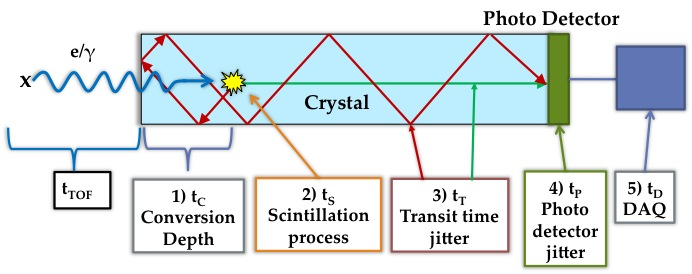
\includegraphics[width=0.85\textwidth]{figs/ScintillatorTiming} \caption{Factors
influencing the precision of the timing measurement with a monolithic, large
scintillating crystal. The incident particle impinges on the crystal face from
the left. Characteristic times of various factors are defined in the colored
boxes and in the text.}
\label{fig:ScintillatorTiming}
\end{figure}

In past studies~\cite{MCPFastCaloNIMA}, we have measured the time resolution
associated with the MCP-PMT photodetectors used in this paper to be
about $11$~ps, and the electronic time resolution
of the DAQ system to be about $6$~ps. By measuring the time
resolution at different absorber thicknesses for electron beams with
energies varying from $12$ to $32$~GeV, we showed that the 
time of arrival of the front of an electromagnetic shower
can be determined with a precision better than $20$~ps.

To complete the characterization of the time resolution
for a crystal based calorimeter, we report here on the results
of studies focusing on the contributions due to fluctuations
in the scintillation process, and in the optical transit
to the photodetector. The signal extracted from the photodetector is 
typically the super-position of the signal generated by many 
scintillation photons arriving together. As a result the effect of 
the fluctuations associated with the creation and transit of 
each particular scintillation photon will be reduced for a LYSO-based 
detector whose signal is the average of a large number of scintillation 
photons. Thus, of particular interest is the dependence of
the time resolution due to fluctuations in the optical transit
with the amount of scintillation light produced.


\section{Experimental Equipment}

A schematic diagram of a typical time of flight measurement
is shown in Figure~\ref{fig:TypicalSchematicDiagram}. All
measurements involve a fast photodetector which serves to
measure the reference ($t_{0}$) timestamp, typically 
an MCP-PMT, and a photodetector further downstream
that detects the signal associated with the
electromagnetic shower from which a simultaneous energy 
and time ($t_{1}$) measurement is made. 

\begin{figure}[H] \centering
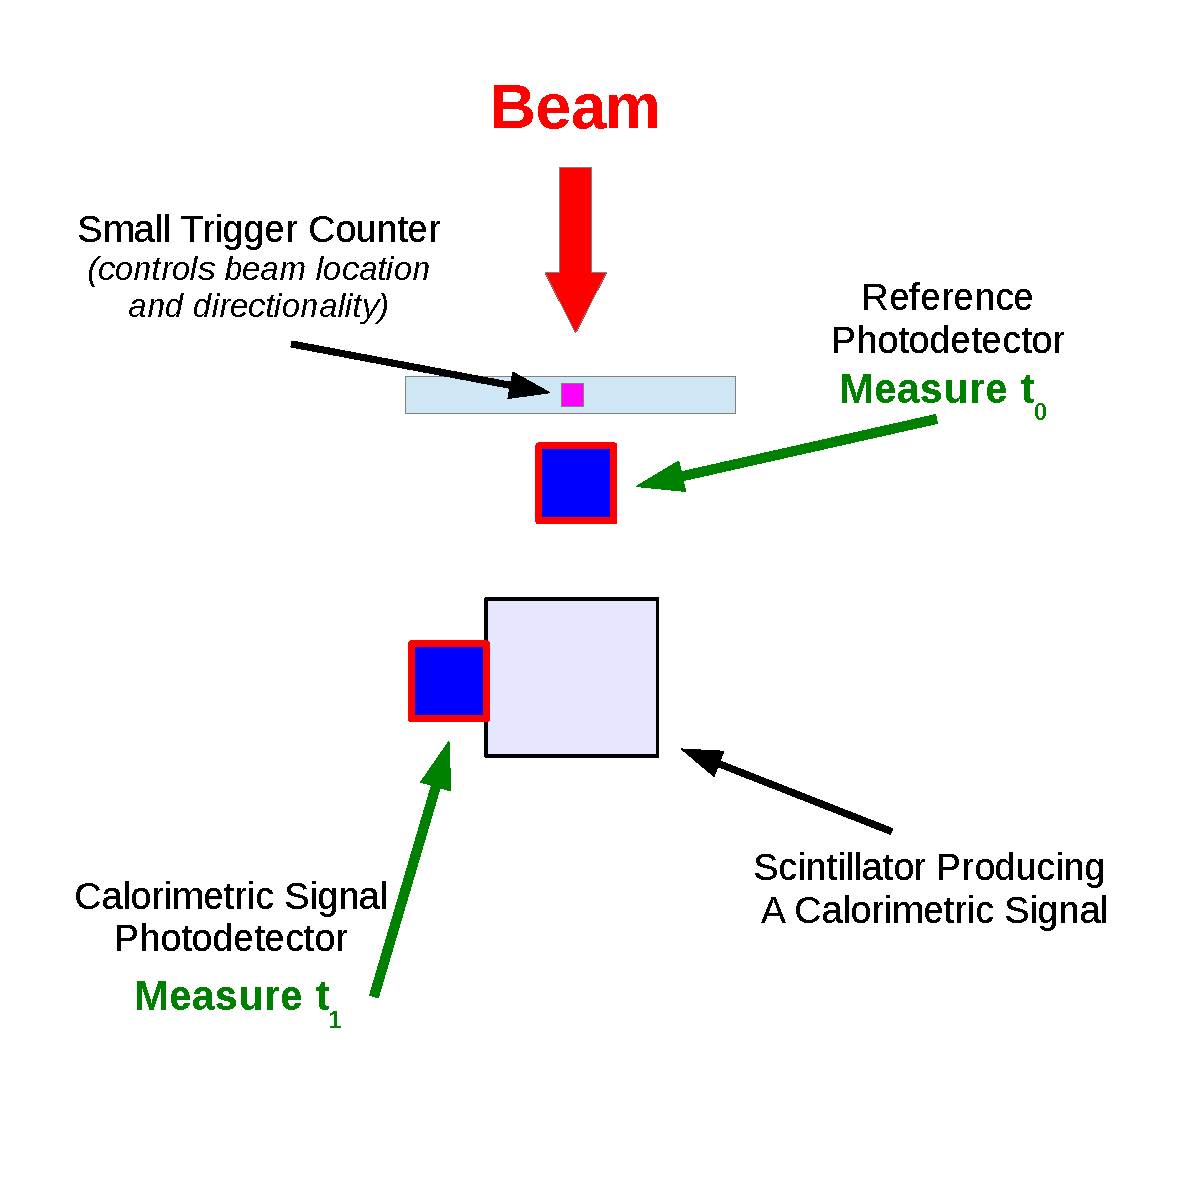
\includegraphics[width=0.45\textwidth]{figs/TypicalSchematicDiagram} 
\caption{A schematic diagram of the experimental setup for
a typical time of flight measurement is shown to illustrate the
basic detector elements.} 
\label{fig:TypicalSchematicDiagram}
\end{figure}

Two types of multi-channel plate photomultiplier
tubes or MCP-PMT photodetectors 
are used, one produced by Hamamatsu 
(model R3809-52)~\cite{HamamatsuMCP3809}, and one
produced by Photek (model PMT240)~\cite{Photek240}. 
A version 4 DRS4 waveform digitizer evaluation board~\cite{DRS4} was
used as the primary DAQ system, connected to a laptop via
USB interface. All experimental beam studies were performed
at the Fermilab Test Beam Facility (FTBF), which 
provided proton beams from the Fermilab Main Injector accelerator
at $120$ GeV, and secondary electron beams of energies ranging 
from $4$ to $32$~GeV. Detector elements were placed inside of a 
dark box lined with copper foil, providing RF shielding. A
$2$x$2$~$\mathrm{mm}^{2}$ scintillator is placed inside the box at
the upstream extremity and used to trigger the DAQ readout,
providing a relatively strict constraint on the location and directionality
of the beam particles used in the time of flight studies. 
Finally, the differential Cherenkov counter located upstream
of our experimental hall, is used for electron identification. 

\section{Event Selection and Analysis}

The analyses performed in these studies primarily involve
reconstructing the time of flight of beam particles
between different detector elements. Slightly different
algorithms are used for different detector elements,
but all involve the assignment of a time stamp using 
specific features of each corresponding signal pulse.
The signal pulse for the reference time detector
is typically very sharp and relatively symmetric 
around its maximum amplitude, as shown in 
Figure~\ref{fig:PulseShapes}. Therefore, for the reference 
detector we determine the time position of the pulse
peak and fit a Gaussian function to the peak
of the pulse, using three sampling points before the 
pulse maximum and four sampling points after. The
mean value of the fitted Gaussian function is
assigned as the timestamp $t_{0}$. The signal pulse
for the downstream time measurement is typically
the result of scintillation light, and exhibits a 
relatively fast rising edge and a significantly slower
decay. Therefore, we assign the timestamp $t_{1}$ 
using a constant fraction fit to the rising edge.
A linear function is fitted between the sampling
points at $10\%$ and $60\%$ of the pulse maximum
and the time stamp is assigned as the time 
at $20\%$ of the pulse maximum on the fitted
linear function. Examples of fits performed to assign a 
time stamp from each pulse are shown in Figure~\ref{fig:PulseFits}.
In both cases, some optimization was performed 
to arrive at the exact algorithm parameters used.

\begin{figure}[h] \centering
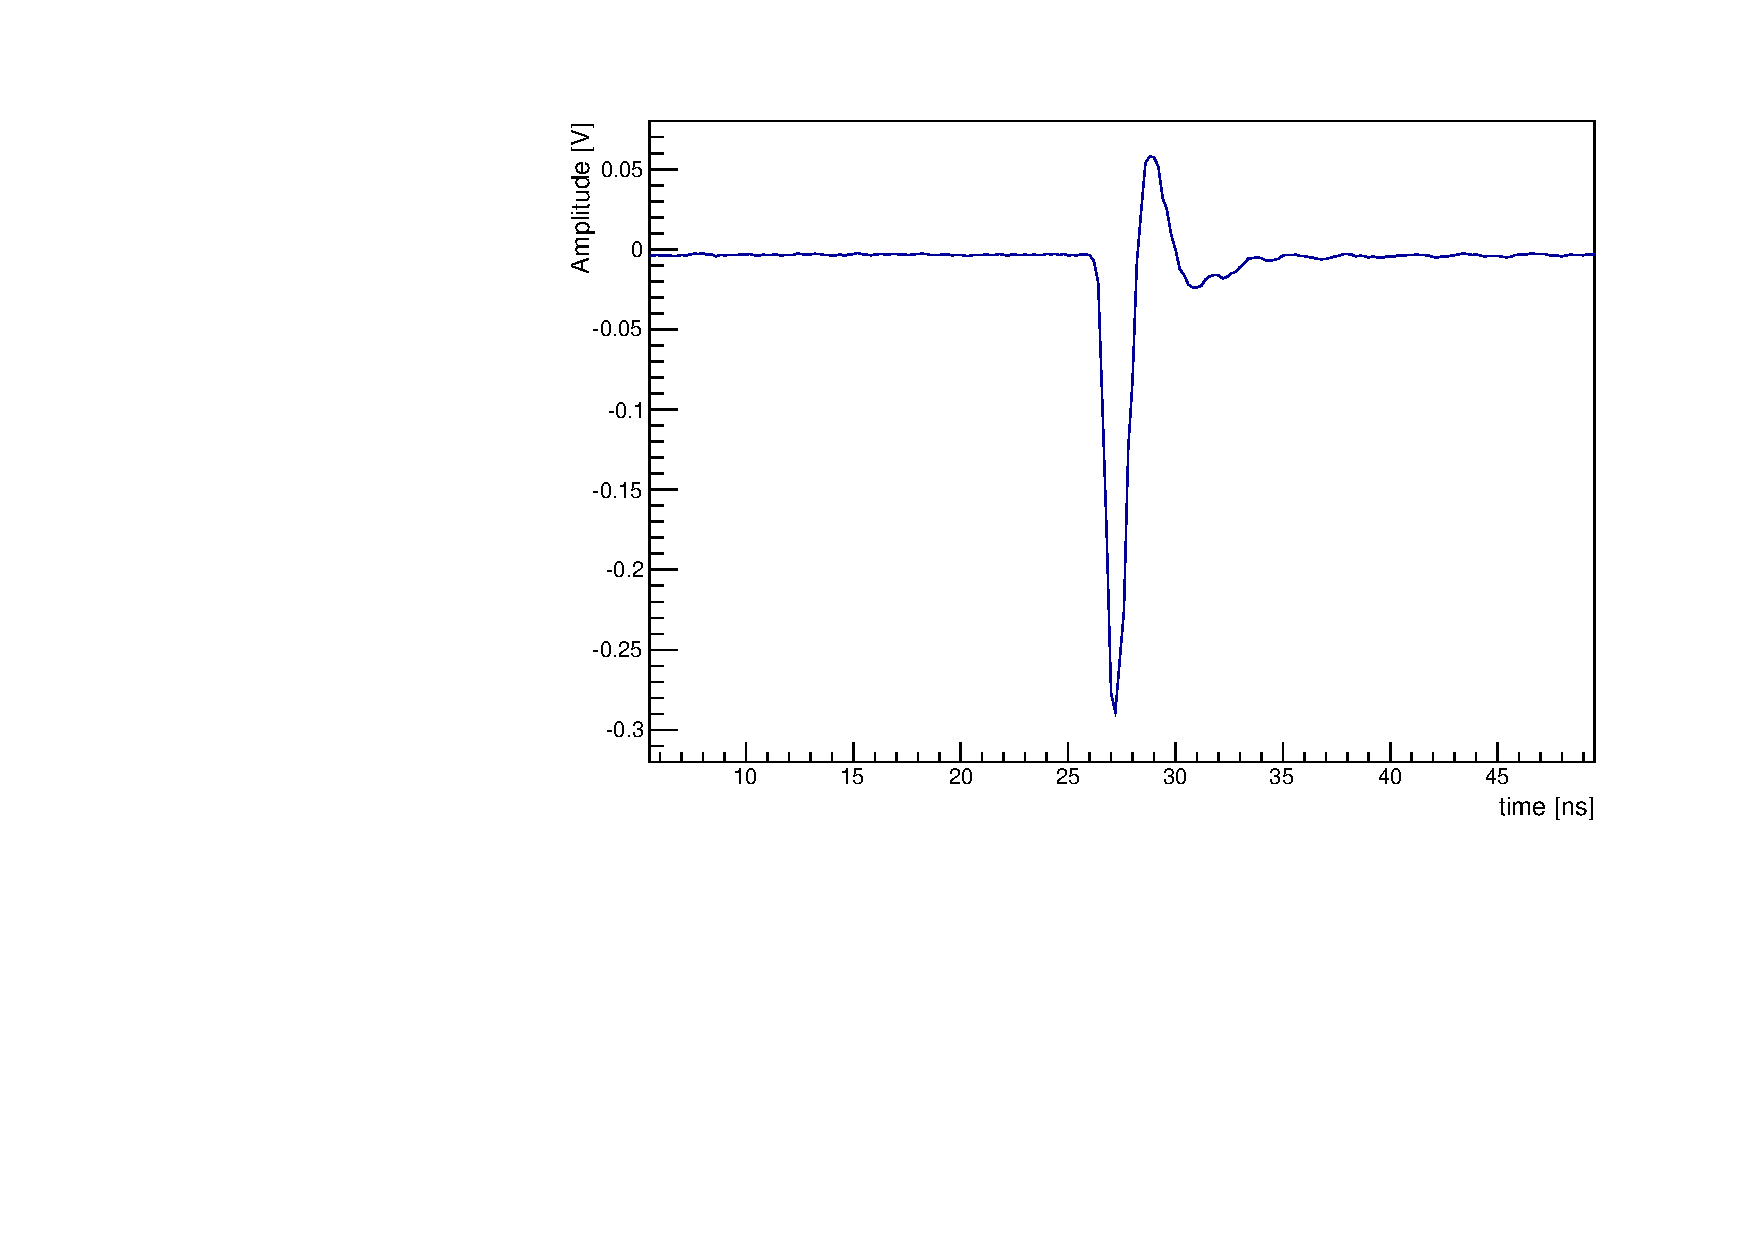
\includegraphics[width=0.45\textwidth]{figs/RefPulse} 
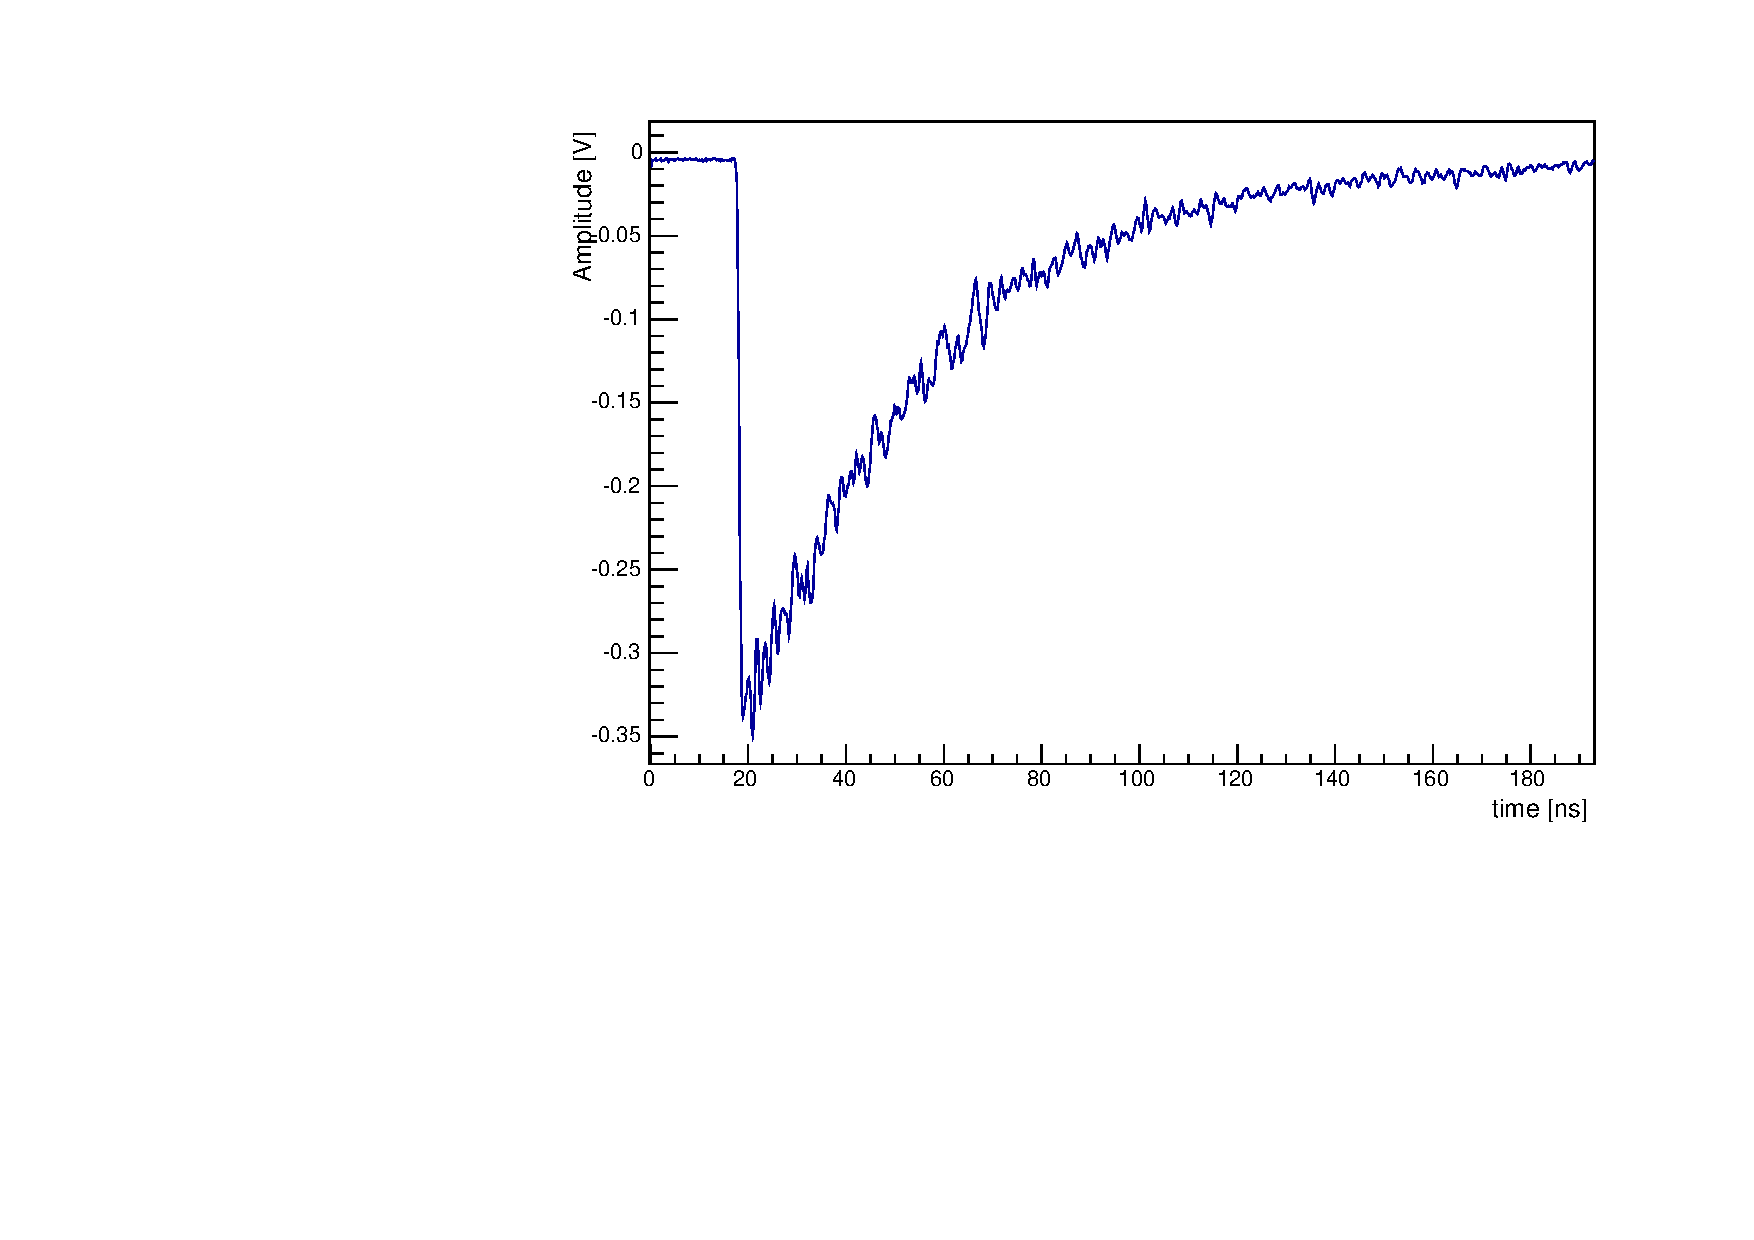
\includegraphics[width=0.45\textwidth]{figs/run064_event506} 
\caption{Sample pulses as digitized by the DRS4 board are shown. 
On the left is a  pulse from the reference Photek 240 MCP-PMT, 
and on the right is a pulse from the Hamamatsu R3809 MCP-PMT
optically coupled to a $(1.7\mathrm{ cm})^3$ LYSO crystal 
from an 8 GeV electron run.} 
\label{fig:PulseShapes}
\end{figure}

Event selection and pulse cleaning procedures were used to eliminate abnormal
pulses in the readout. Large signals above 500 mV were also rejected because
they saturated the DRS4 inputs. Only pulses with amplitude 
larger than 20 mV were used for time of flight measurements in order to 
avoid any impact of the noise from the DRS waveform digitizer DAQ system. 
Events containing more than one pulse within our readout window of 200 ns 
were not used. 

\begin{figure}[h] \centering
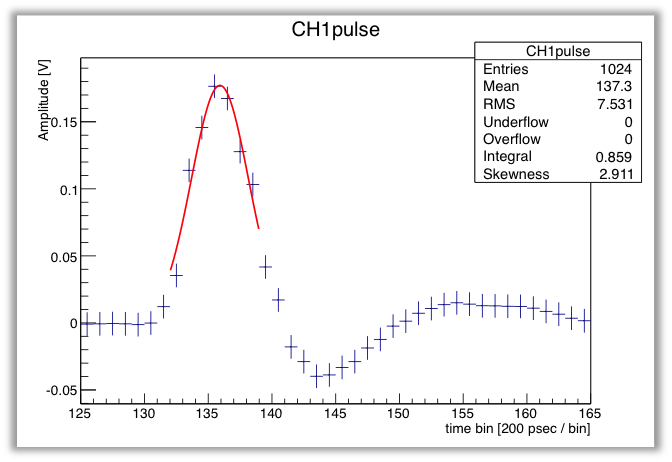
\includegraphics[width=0.45\textwidth]{figs/RefPulseFit} 
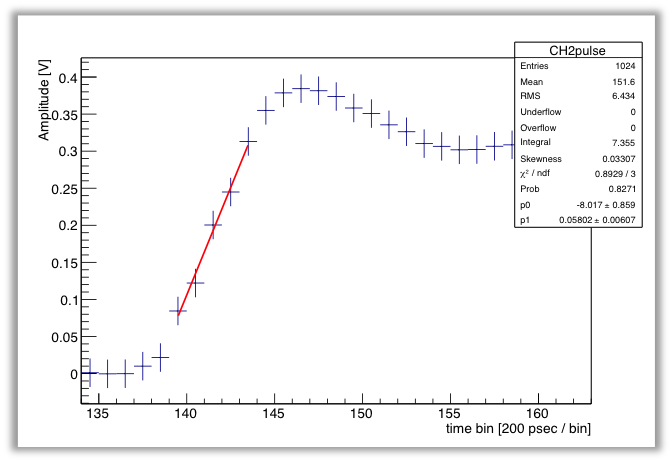
\includegraphics[width=0.45\textwidth]{figs/ScintPulseFit} 
\caption{Sample fits to assign a time stamp to each pulse is shown. 
On the left is a pulse from the reference Photek 240 MCP-PMT, and
on the right is a pulse from the Hamamatsu R3809 MCP-PMT
optically coupled to a $(1.7\mathrm{ cm})^3$  LYSO crystal
from an 8 GeV electron run.}
\label{fig:PulseFits}
\end{figure}


\section{Timing in LYSO Crystal-based Calorimeters}

As we discussed in the introduction, this article describes studies
focused on the characterization of two of the five main aspects
driving the time resolution: scintillation and 
optical transport. Stochastic processes in the scintillation
mechanism and the randomization of the optical paths for the 
scintillation light to reach the location of the photodetector 
affect both the speed of the signal formation
as well as the time jitter. We characterize the impact of
these two effects on the time resolution using
two independent experimental setups which isolate the
two components. To study the effect of scintillation
we perform time resolution measurements
for electron beams using a sampling calorimeter composed of a 
$(1.7\mathrm{ cm})^{3}$ LYSO cube as the active 
scintillating element behind about $4.5$ radiation lengths of lead. 
The effect of optical transport is studied by measuring
the time resolution using a shashlik 
calorimeter composed of alternating layers of tungsten
and LYSO, with scintillation light signal extracted
through wavelength shifting fibers as well as 
through direct optical coupling to the edges of a few
LYSO layers. 


\subsection{Studies of Scintillation Time Jitter}

We study the impact of the scintillation mechanism in LYSO
on the time resolution using a simple 
sampling calorimeter composed of a layer of
lead, about $4.5$ radiation lengths in thickness, acting
as a radiator and a LYSO crystal cube with linear dimensions 
of $1.7$~cm. The LYSO crystal is wrapped in Tyvek and  
coupled with optical grease to a Hamamatsu R3809 MCP-PMT
which is used to extract the scintillation signal. 
A Photek 240 MCP-PMT is placed upstream of the calorimeter and 
is used to measure the reference time. A schematic diagram
and a photograph of the experimental setup
is shown in Figure~\ref{fig:LYSOSamplingCaloSetup}. 
The contribution of optical transit effects on the 
time resolution is reduced in this setup.

\begin{figure}[h] \centering
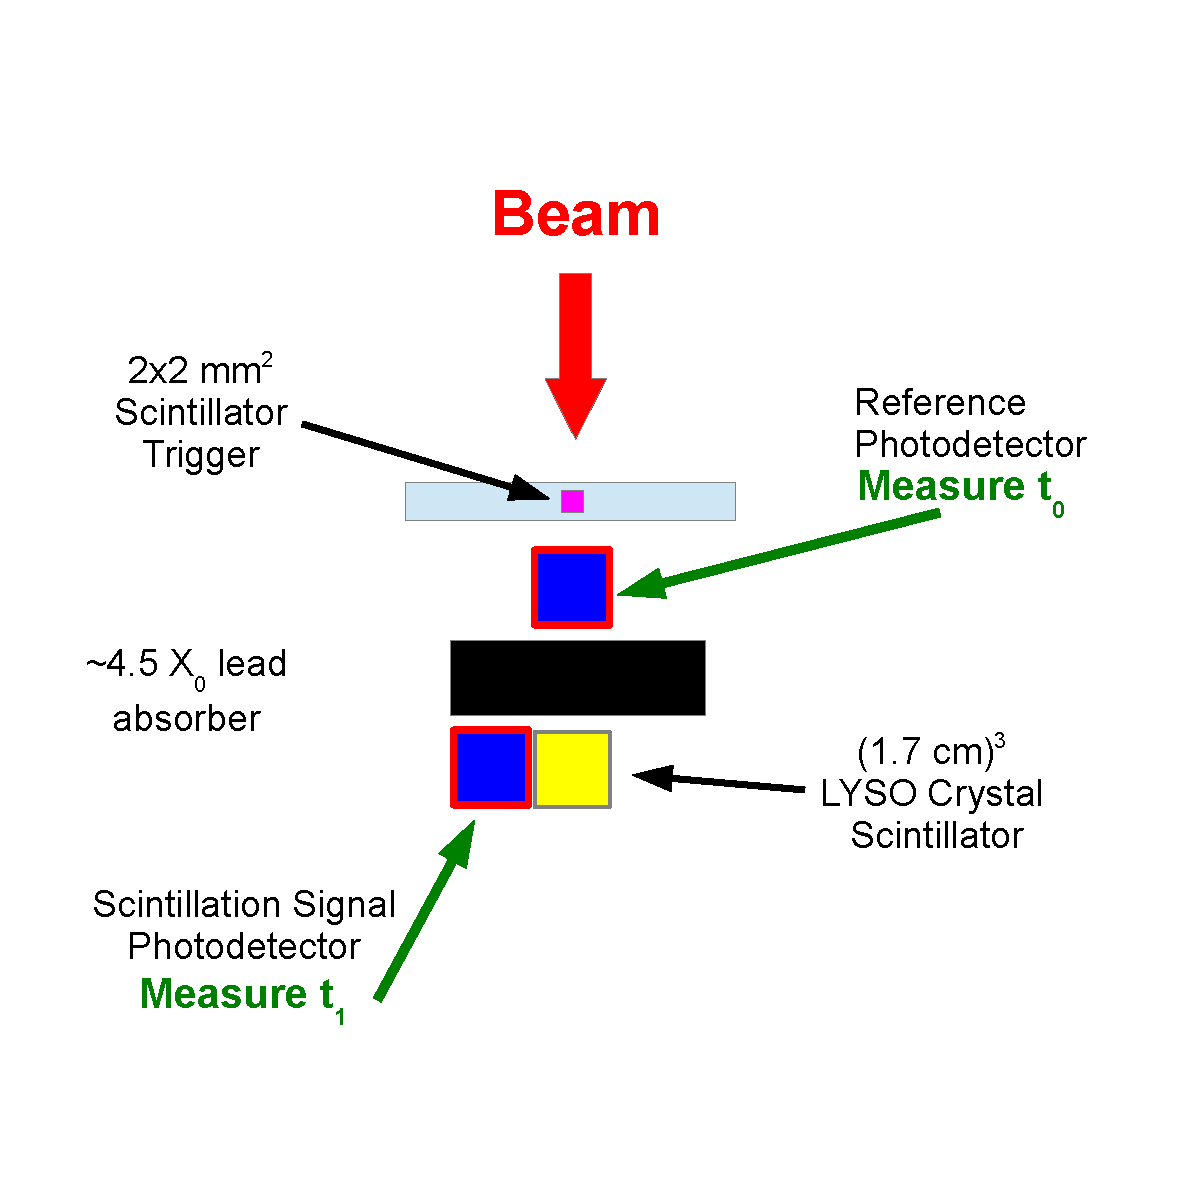
\includegraphics[width=0.45\textwidth]{figs/LYSOSamplingCaloSetupSchematic} 
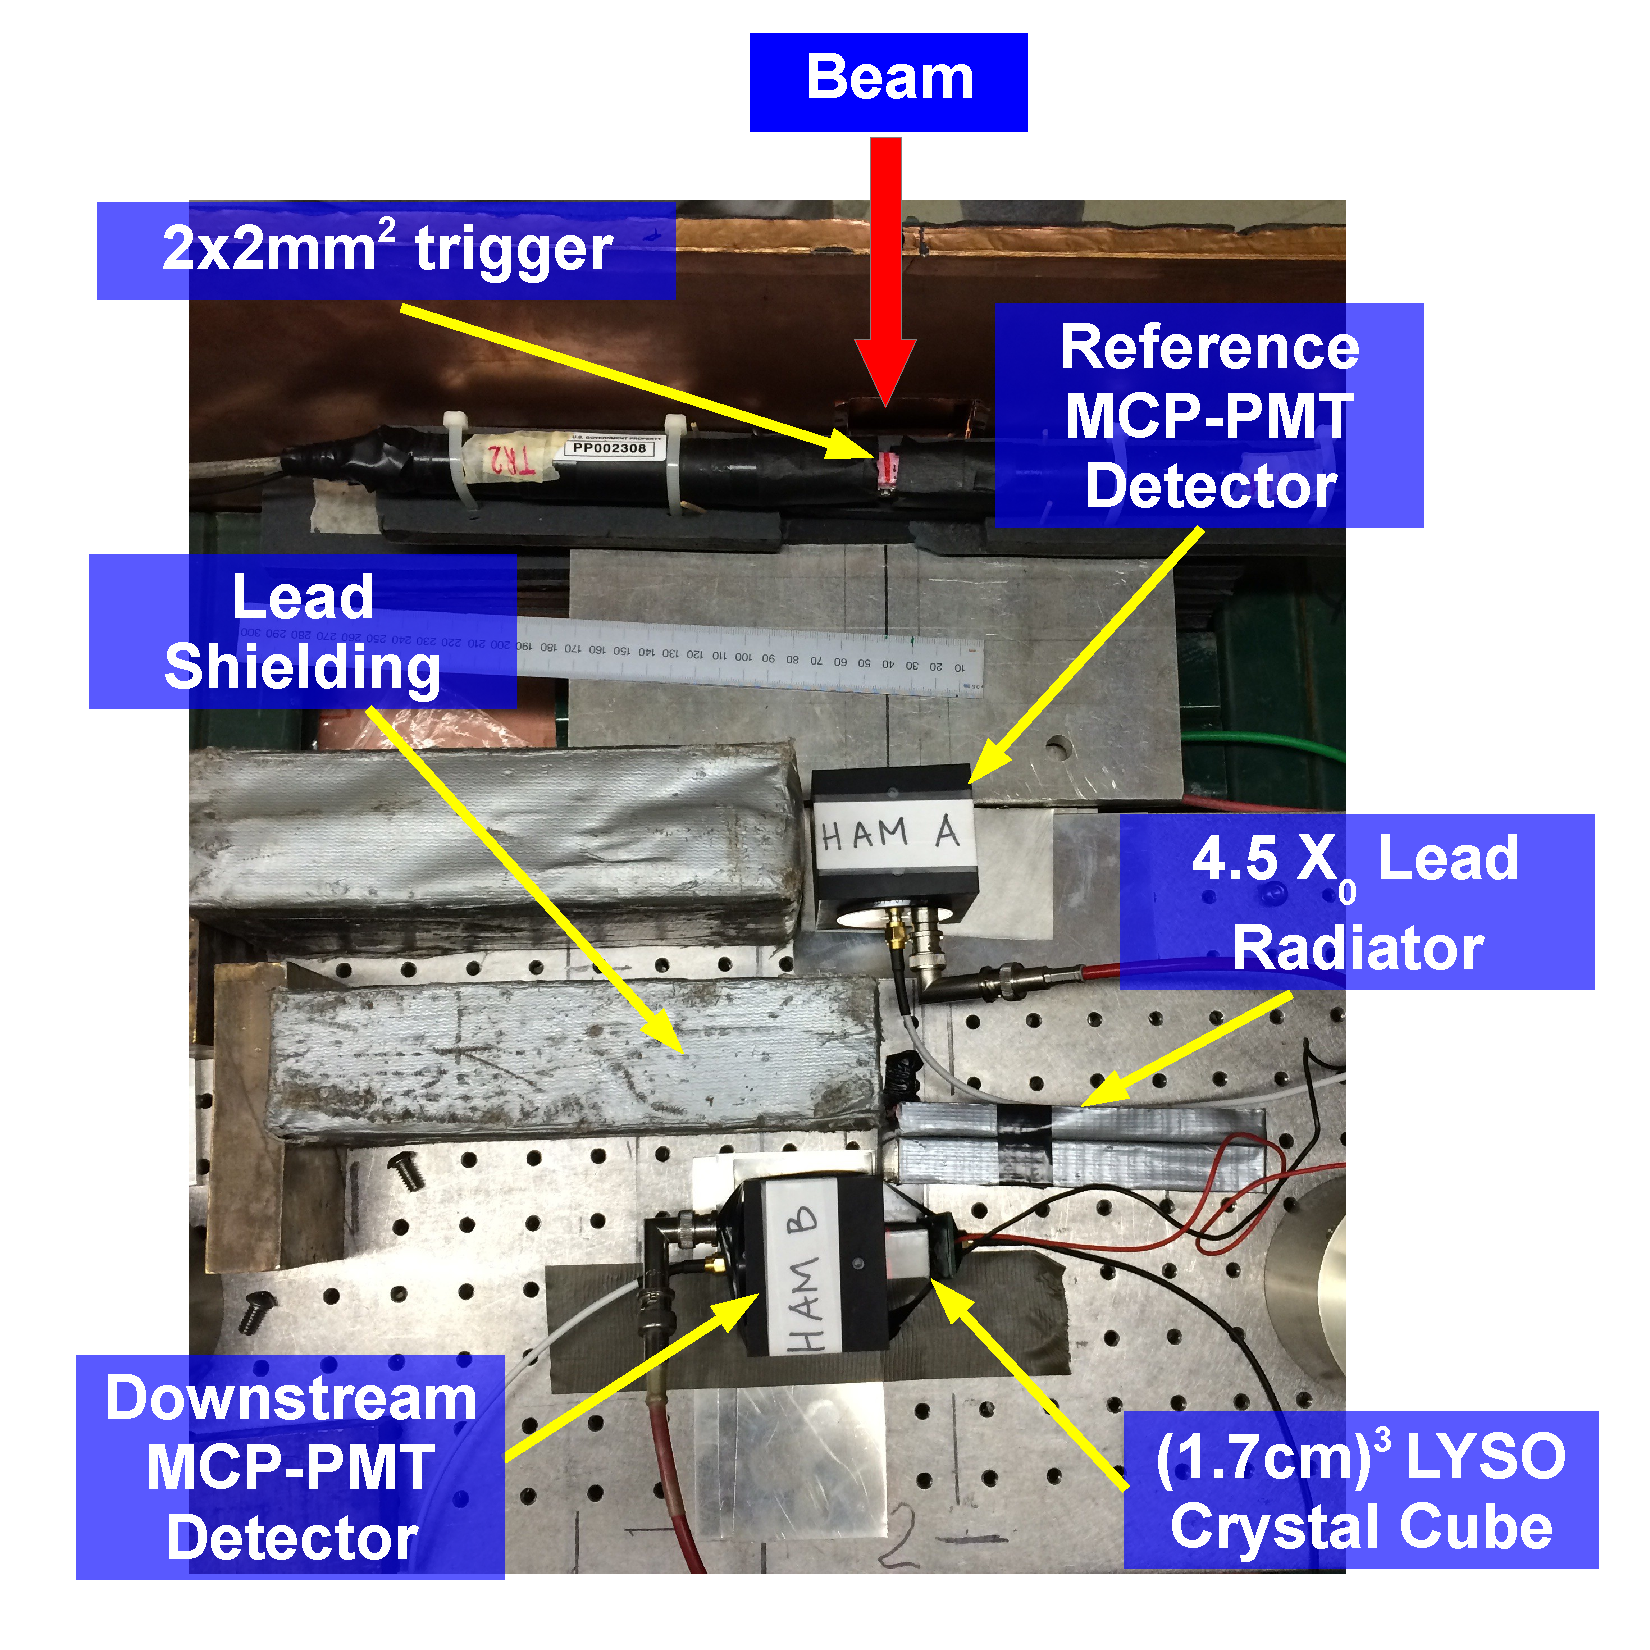
\includegraphics[width=0.45\textwidth]{figs/LYSOSamplingCaloSetupPhoto} 
\caption{ A schematic diagram of the experimental setup for the
time of flight measurement using the LYSO sampling calorimeter
is shown, along with a photograph of the experimental setup. } 
\label{fig:LYSOSamplingCaloSetup}
\end{figure}

A plastic scintillator, approximately $2$~mm by $2$~mm in cross sectional area
and placed upstream of the reference time detector, is used to trigger
the DAQ readout on the DRS waveform digitizer and ensures that any
time of flight measurement is constrained to within a $2$~mm region,
which limits the time jitter due to the geometry to about $12$~ps, assuming that
the speed of light inside LYSO is $\sim 1/2$c. 
Electron events are identified by requiring a signal with amplitude
larger than $10$~mV in the Cherenkov counter.
Finally, large lead bricks are placed upstream of the Hamamatsu
R3809 MCP-PMT but out of the beam to provide shielding of the photodetector
from stray particles produced from events where an electromagnetic shower
occurred elsewhere upstream of the lead radiator. Such stray shower
events yield very fast signals which can significantly contaminate the
scintillation signal if left uncontrolled. Using the identical
experimental setup but without the LYSO active element in place,
we found that stray shower type events yield less than $10\%$ contamination
and gives a negligible effect on the scintillation signal. The same calorimeter
setup using the Photek 240 MCP-PMT in place of the Hamamatsu R3809 MCP-PMT,
which has an active area about $10$ times larger, was found to yield 
more than $80\%$ contamination and thus did not result in a proper
measurement of the scintillation signal.

Despite the thickness of the LYSO active element layer being relatively
small and therefore only capturing a fraction of the total energy
of the electron, the location of the active element is relatively close to the
shower maximum for electromagnetic showers, and yields
a reasonable energy measurement. In Figure~\ref{fig:LYSOCubeEnergy32GeV}
we show the distribution of the pulse integral, a quantity
proportional to the total collected charge, for events
measured by this sampling calorimeter produced with a
$32$~GeV electron beam, and find a resolution of about $20\%$.


\begin{figure}[h] \centering
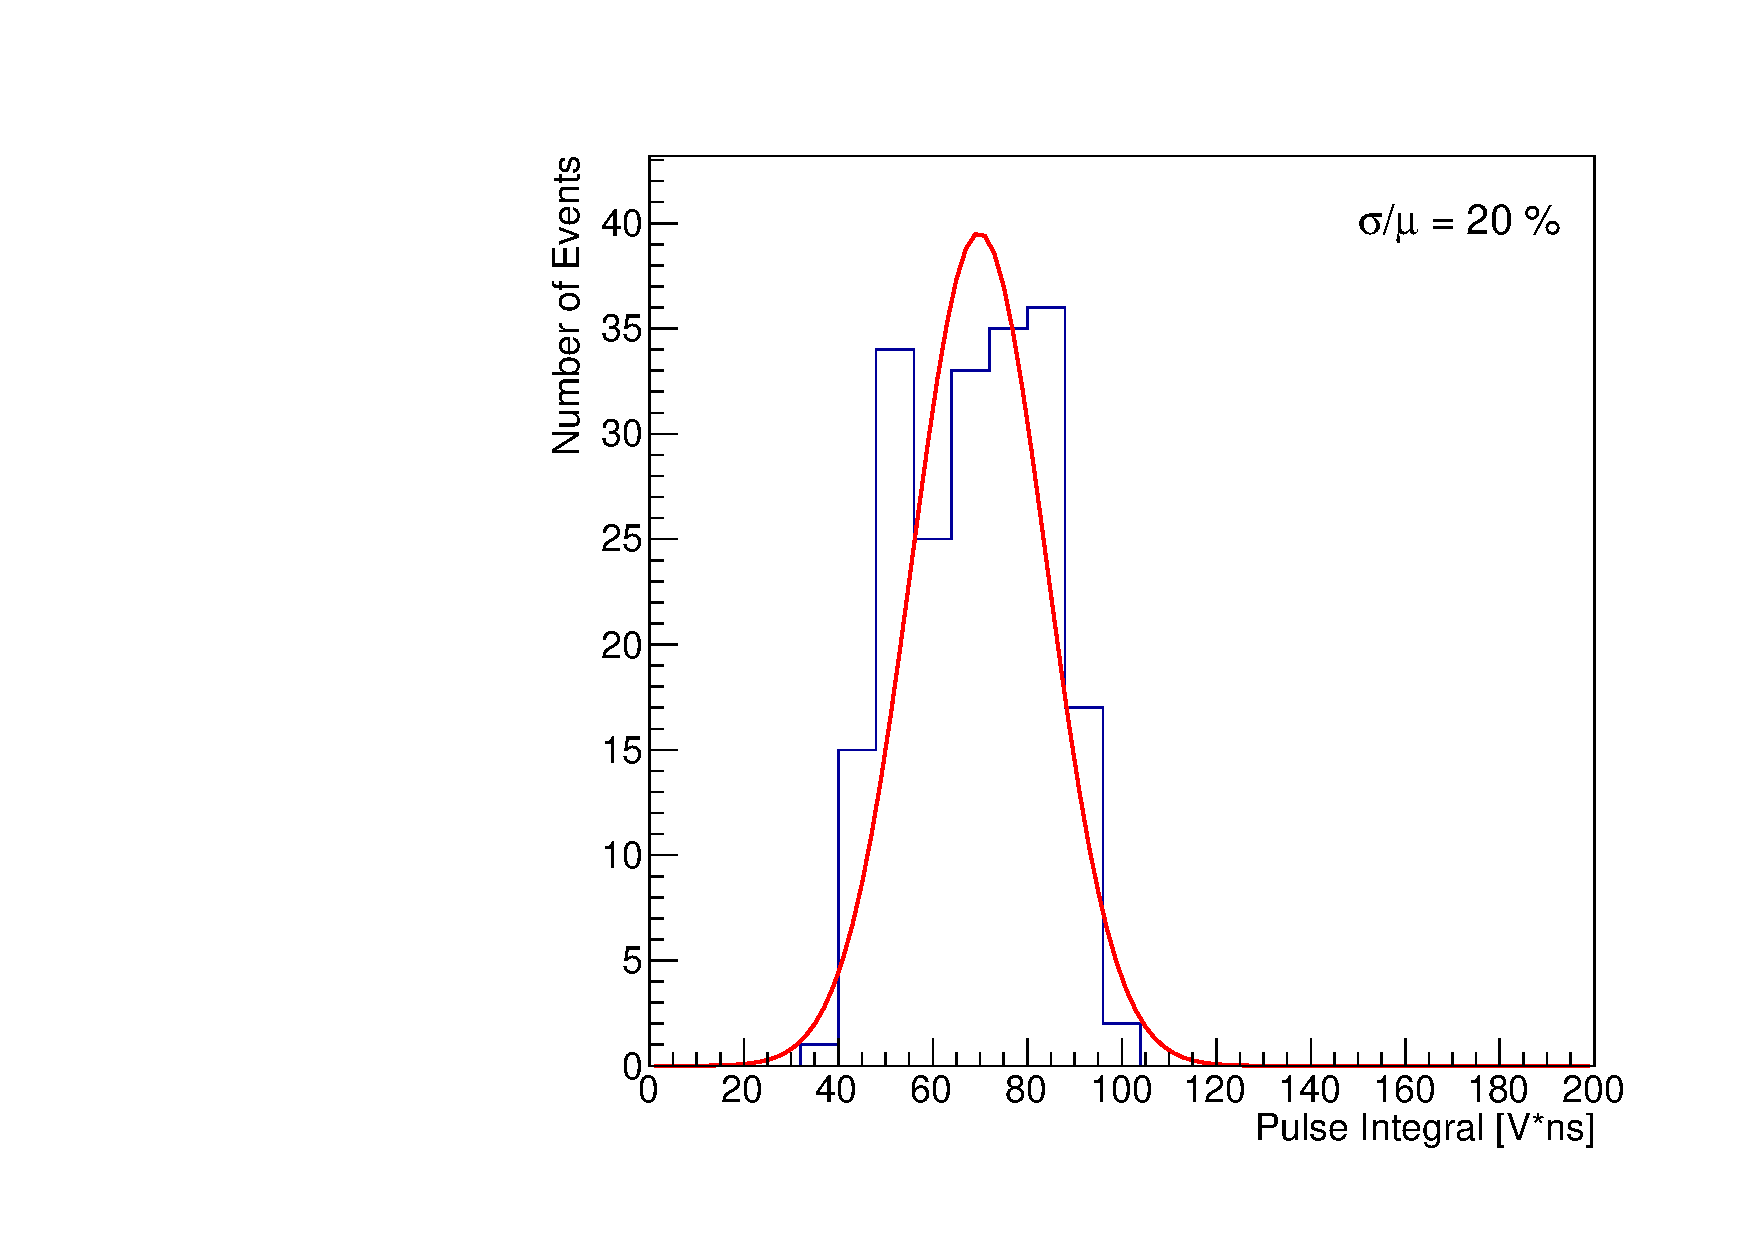
\includegraphics[width=0.45\textwidth]{figs/TOF_Electron_LYSOCube_32GeV_energy} 
\caption{ Histogram of the pulse integral for events recorded using
the LYSO cube sampling calorimeter for a $32$~GeV electron beam. } 
\label{fig:LYSOCubeEnergy32GeV}
\end{figure}

The time of flight measurement was performed using the LYSO sampling calorimeter
for electron beams with energies varying from $4$~GeV to $32$~GeV. The 
measured time of flight distributions are shown in Figure~\ref{fig:LYSOCubeTOF}.
We achieve the best time resolution of $34$~ps for electrons
with beam energy of $32$~GeV.

\begin{figure}[H] \centering
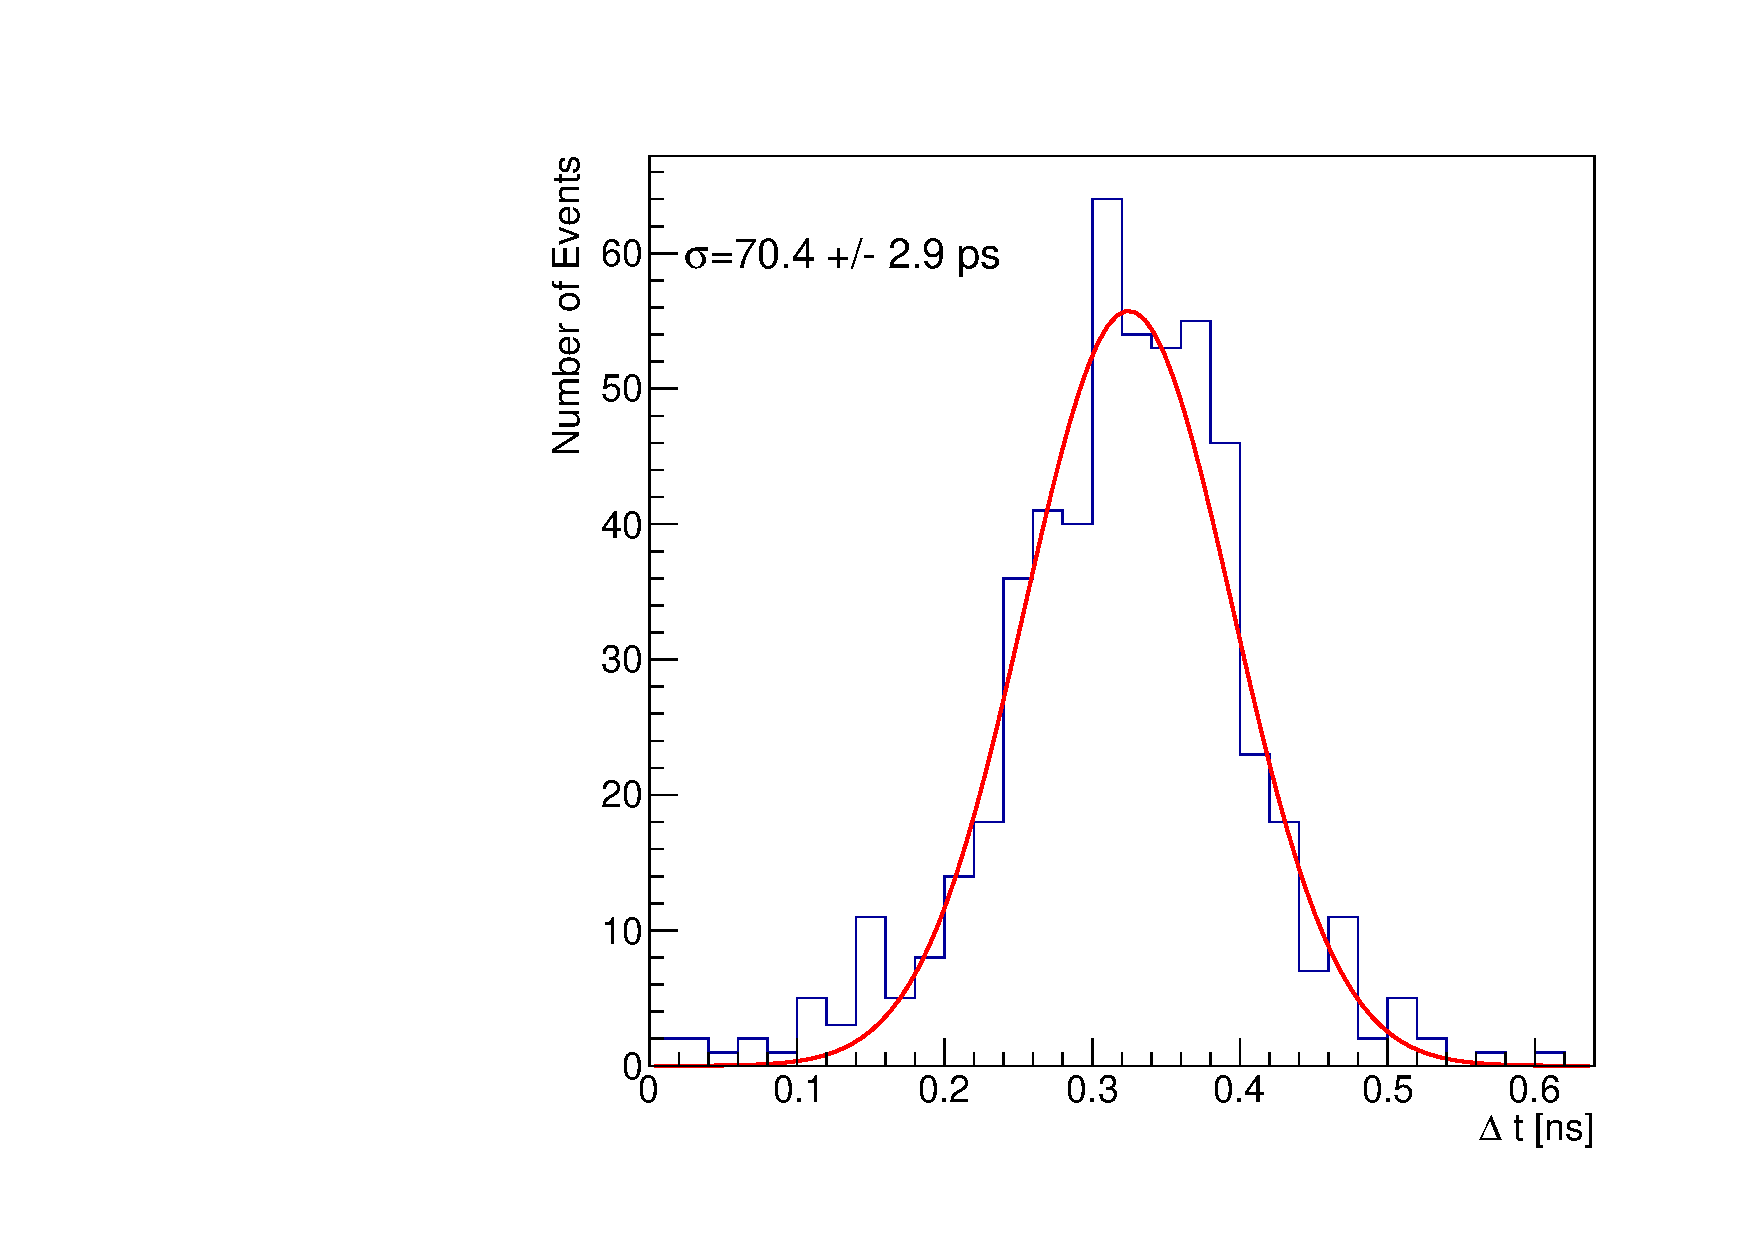
\includegraphics[width=0.45\textwidth]{figs/TOF_Electron_LYSOCube_4GeV} 
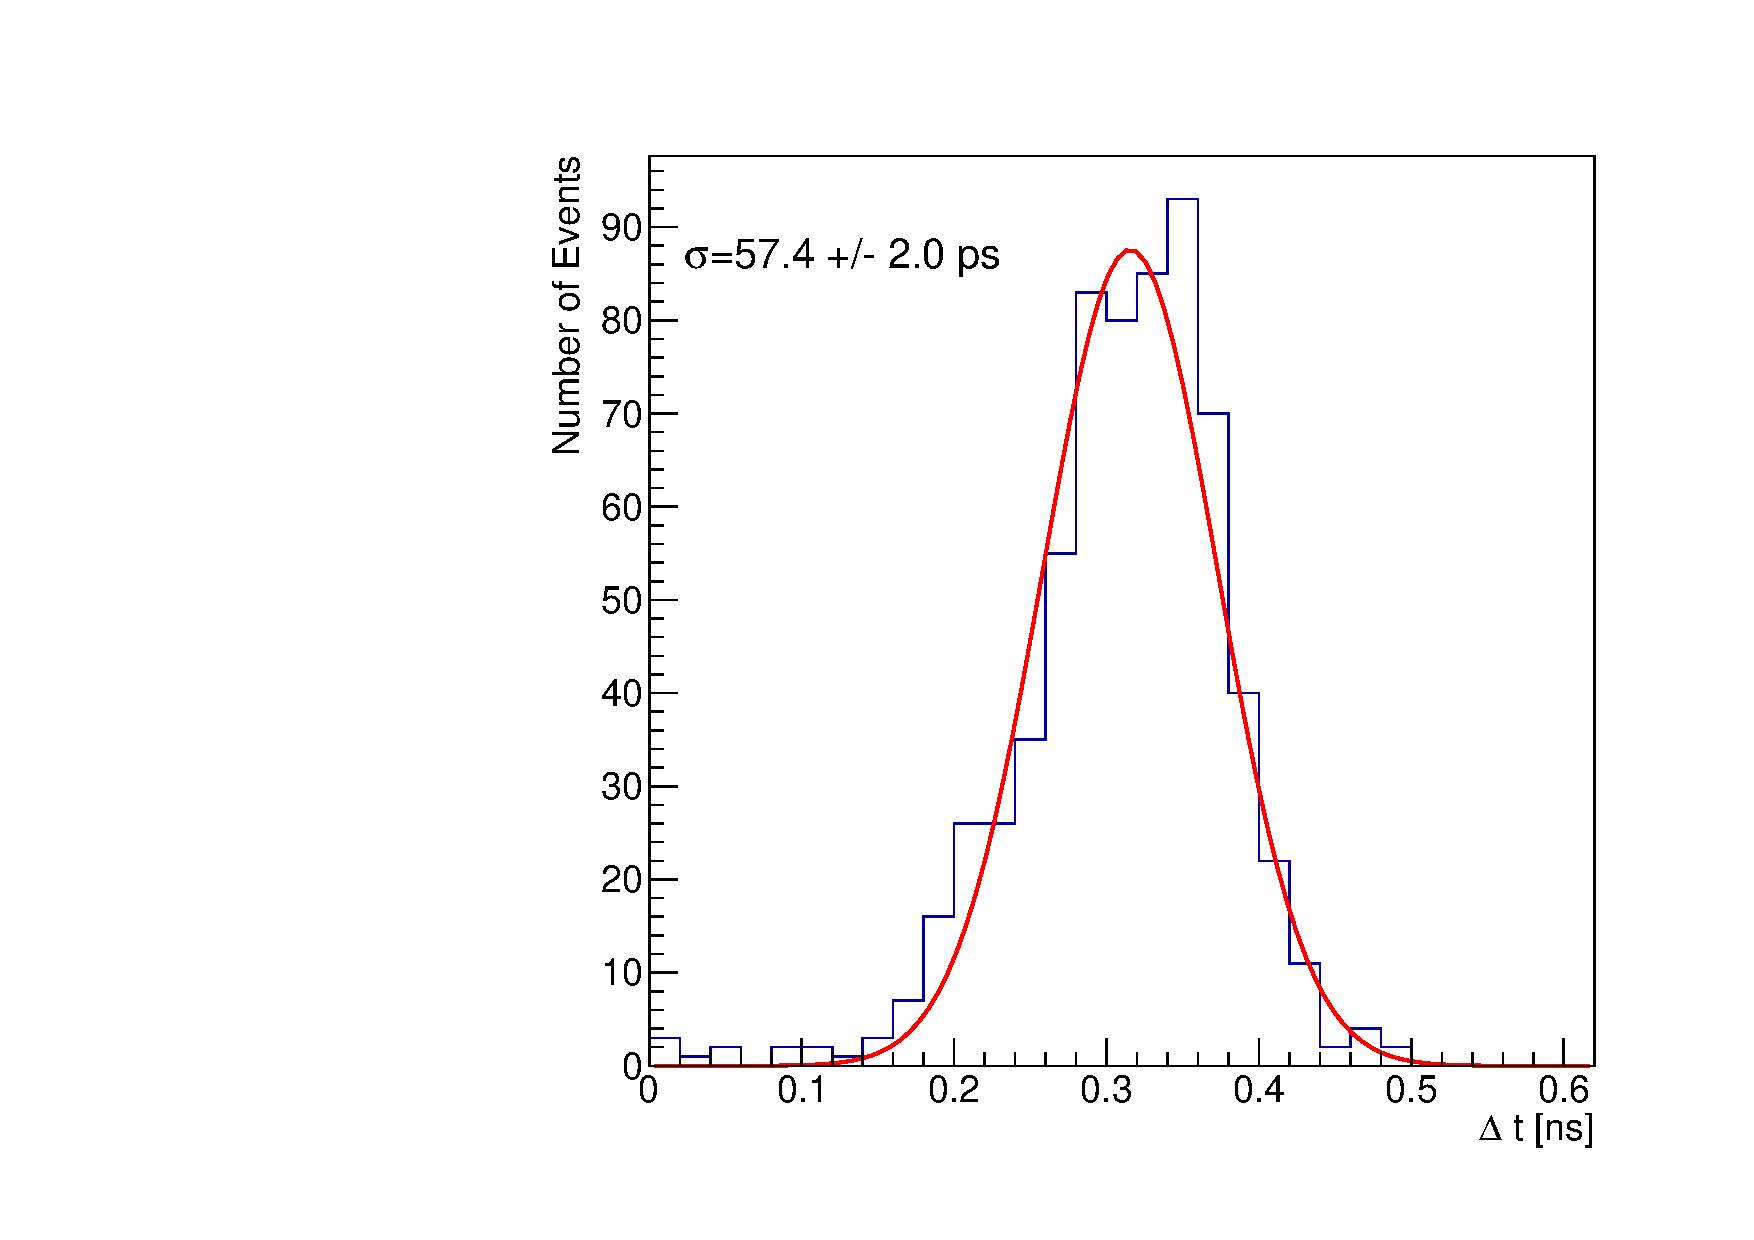
\includegraphics[width=0.45\textwidth]{figs/TOF_Electron_LYSOCube_8GeV} 
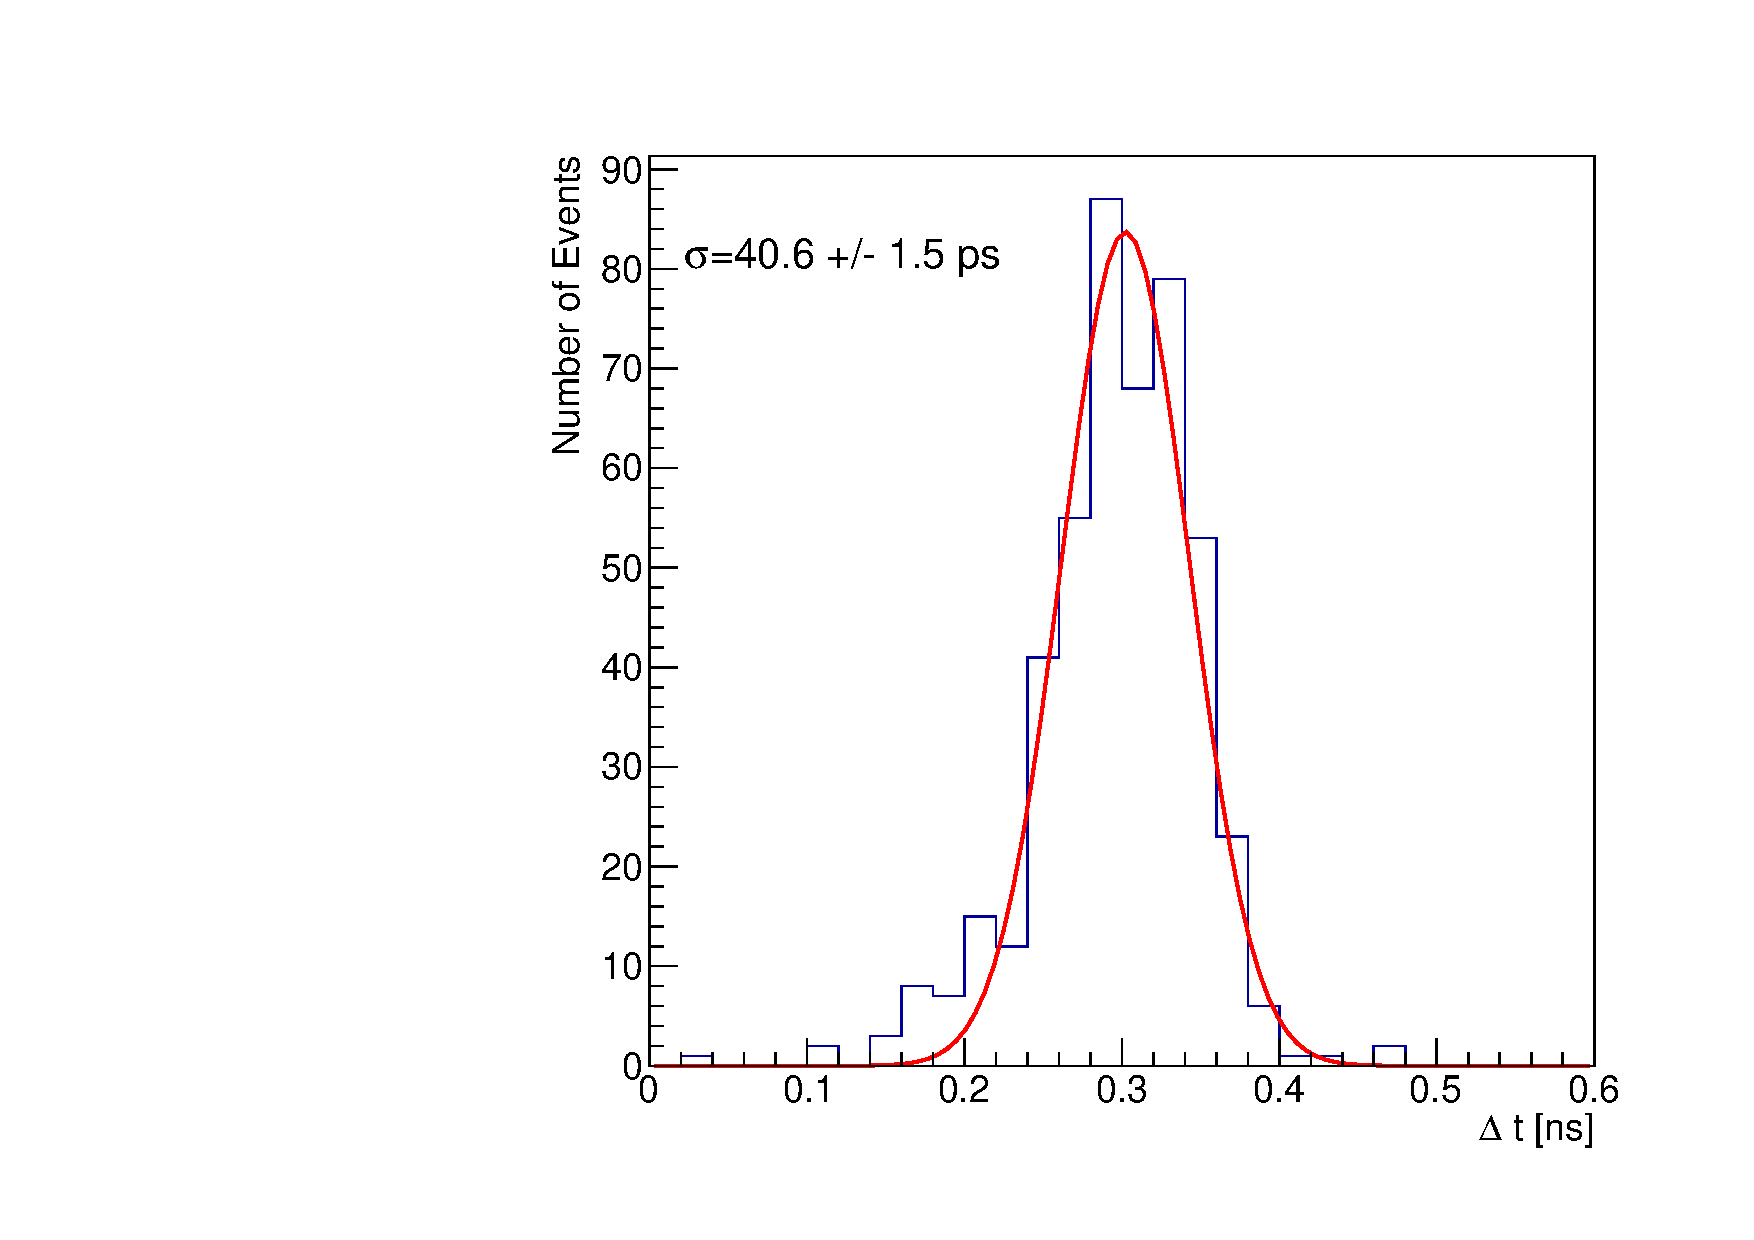
\includegraphics[width=0.45\textwidth]{figs/TOF_Electron_LYSOCube_16GeV} 
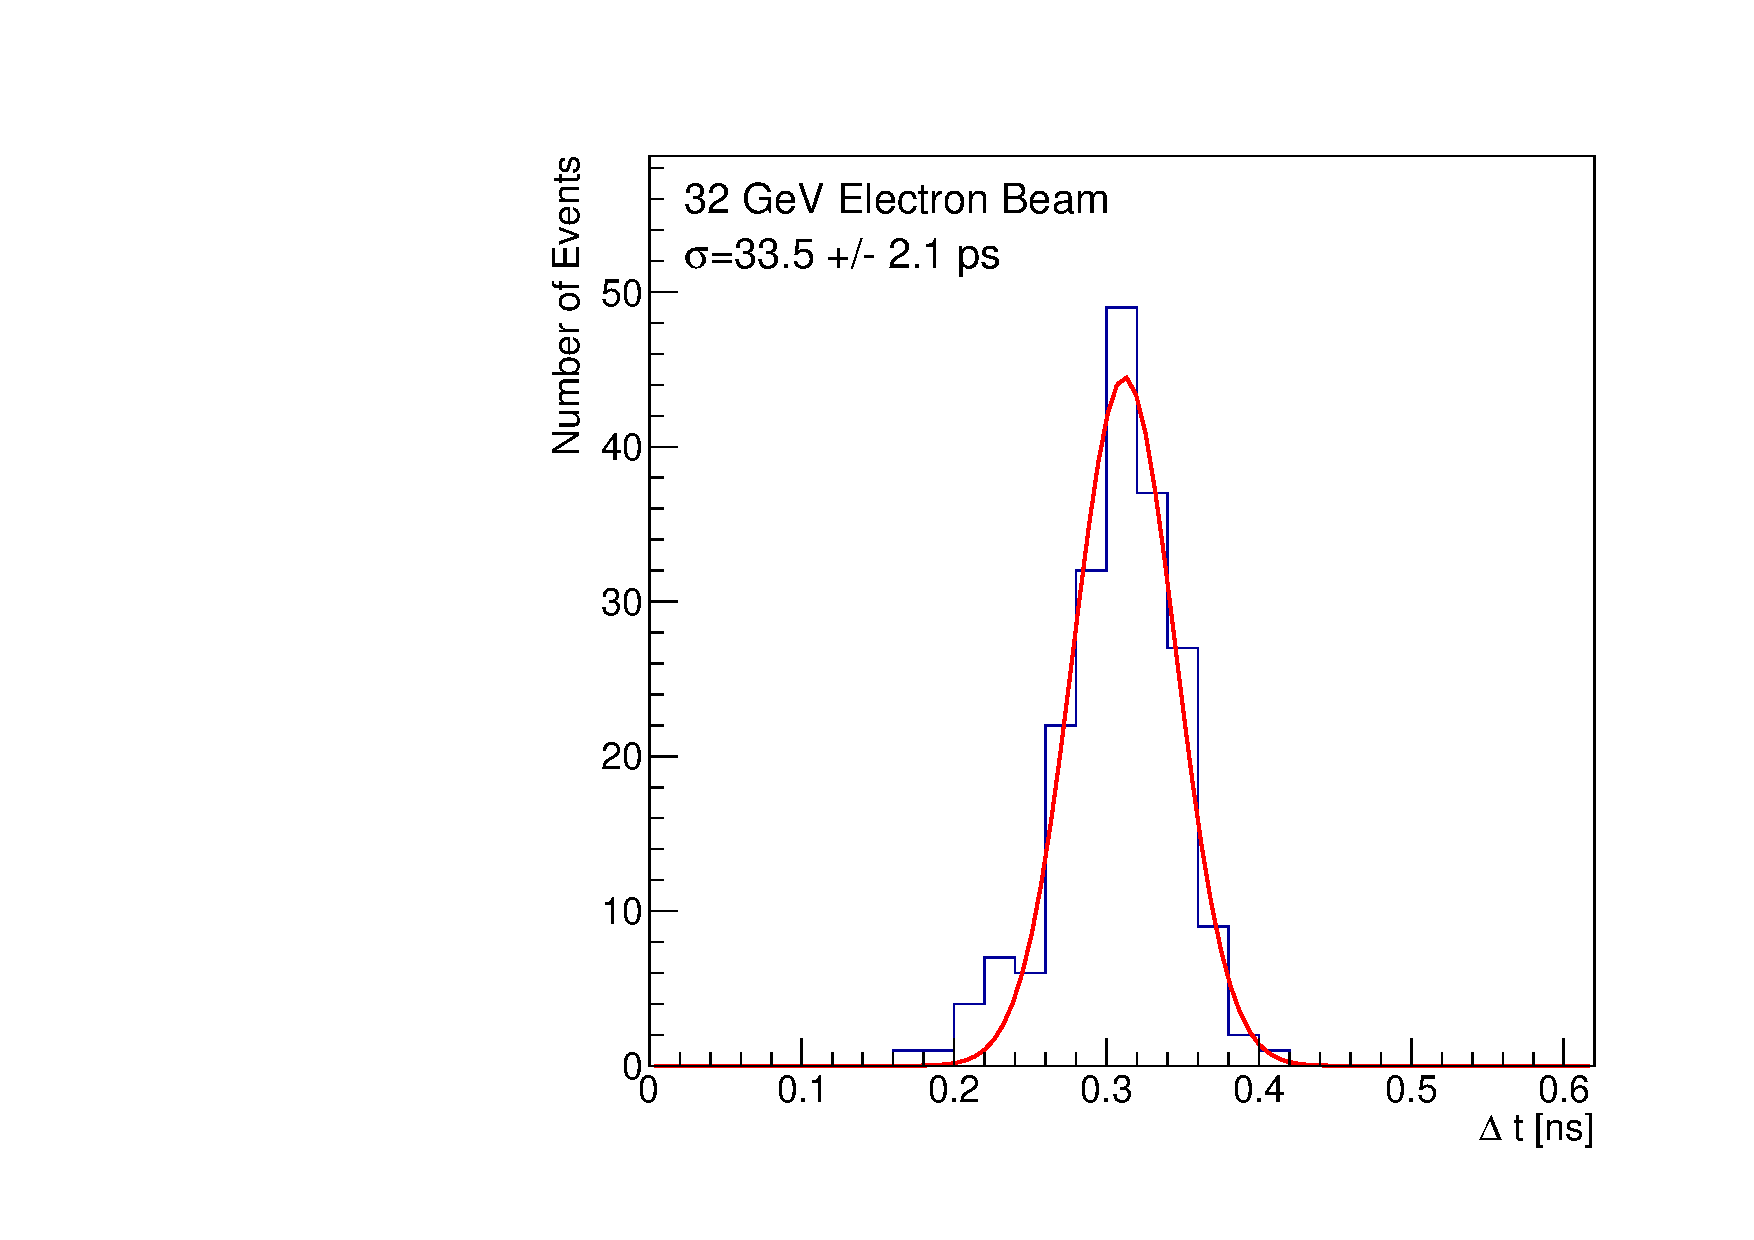
\includegraphics[width=0.45\textwidth]{figs/TOF_Electron_LYSOCube_32GeV} 
\caption{ Time of flight distributions for the LYSO cube sampling calorimeter
for electron beams with varying beam energies. } 
\label{fig:LYSOCubeTOF}
\end{figure}

The time resolution measurements are plotted as a function of the
beam energy in Figure~\ref{fig:LYSOCubeTOFResolutionVsEnergy}, and are observed
to follow a $1/\sqrt{E}$ dependence. We fit the result to the sum of a 
$1/\sqrt{E}$ term and a constant term, and determine the constant term to
be about $11$~ps with a statistical uncertainty of about $30\%$. 

\begin{figure}[h] \centering
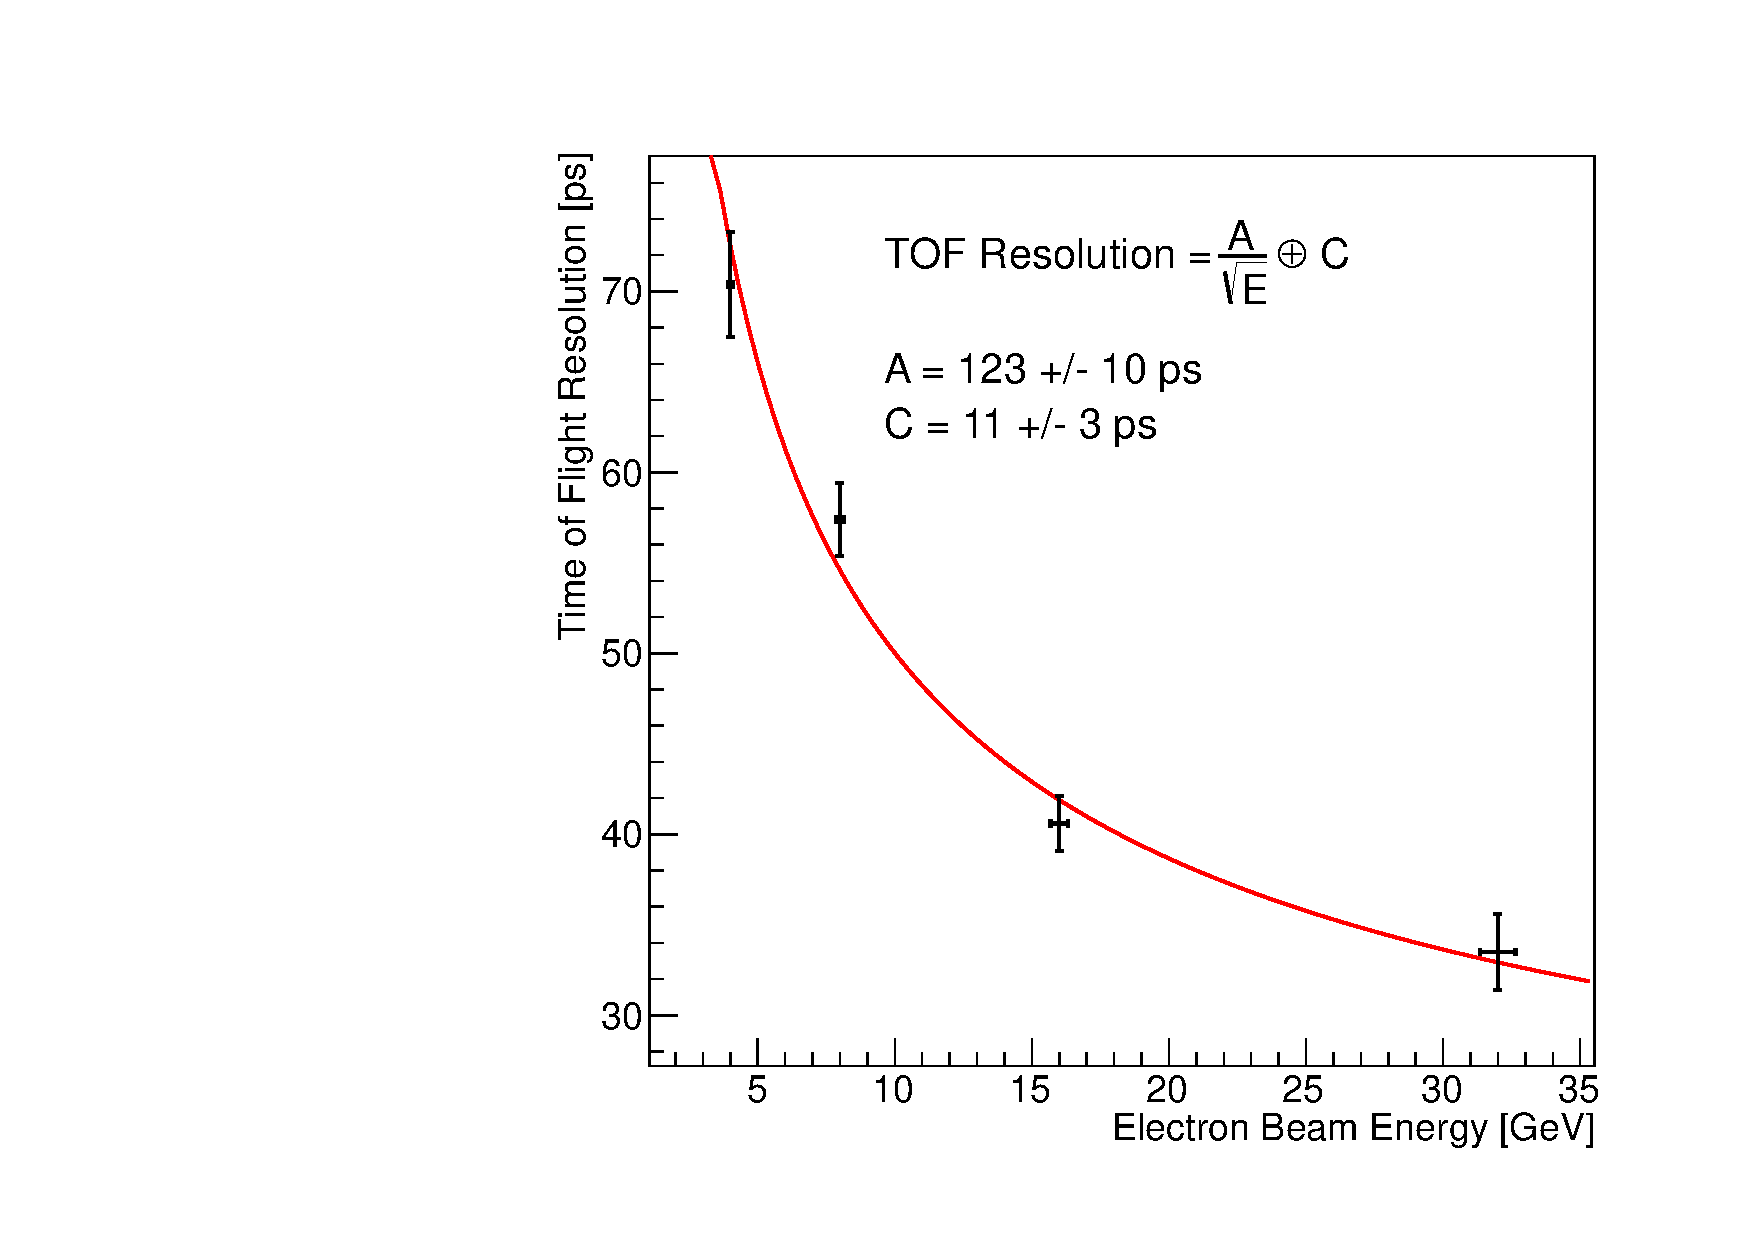
\includegraphics[width=0.45\textwidth]{figs/TimeResolutionVsEnergy_CrystalCube} 
\caption{ The time resolution measured using the LYSO cube
sampling calorimeter is plotted as a function of the electron beam energy, 
and fitted to the sum of a $1/\sqrt{E}$ term and a constant term. Note that the energy absorbed in the LYSO cube is a small fraction of the incident electron energy.}
\label{fig:LYSOCubeTOFResolutionVsEnergy}
\end{figure}

Given that we control the combined contribution to the time 
resolution of the electromagnetic shower
fluctuations, the photodetector time resolution, and the DAQ electronics
to about $25$~ps~\cite{MCPFastCaloNIMA} and that the geometric contribution 
from the transverse size of the trigger is about $12$~ps,
we infer that the contribution of the scintillation mechanism in LYSO
to the time resolution is less than $20$~ps.


\subsection{Studies of Time Jitter from Optical Transport}

We study the contribution to the time resolution due to
various forms of optical transport in the context of a LYSO-tungsten Shashlik
calorimeter, one of the proposed choices for the Phase 2 upgrade of the
CMS endcap calorimeter system. We compare the time  resolution
performance for two alternative optical transport schemes. 

We begin with a conventional scheme where scintillation light is collected
by wavelength shifting fibers through a set of four holes penetrating 
the LYSO layers. A schematic diagram and a photograph showing this setup 
are shown in Figure~\ref{fig:ShashlikFiberSetup}. 
MCP-PMT's produced by Hamamatsu (R3809) are used to collect 
the scintillation light, while a Photek 240 MCP-PMT is used as the reference 
time detector. 


\begin{figure}[H] \centering
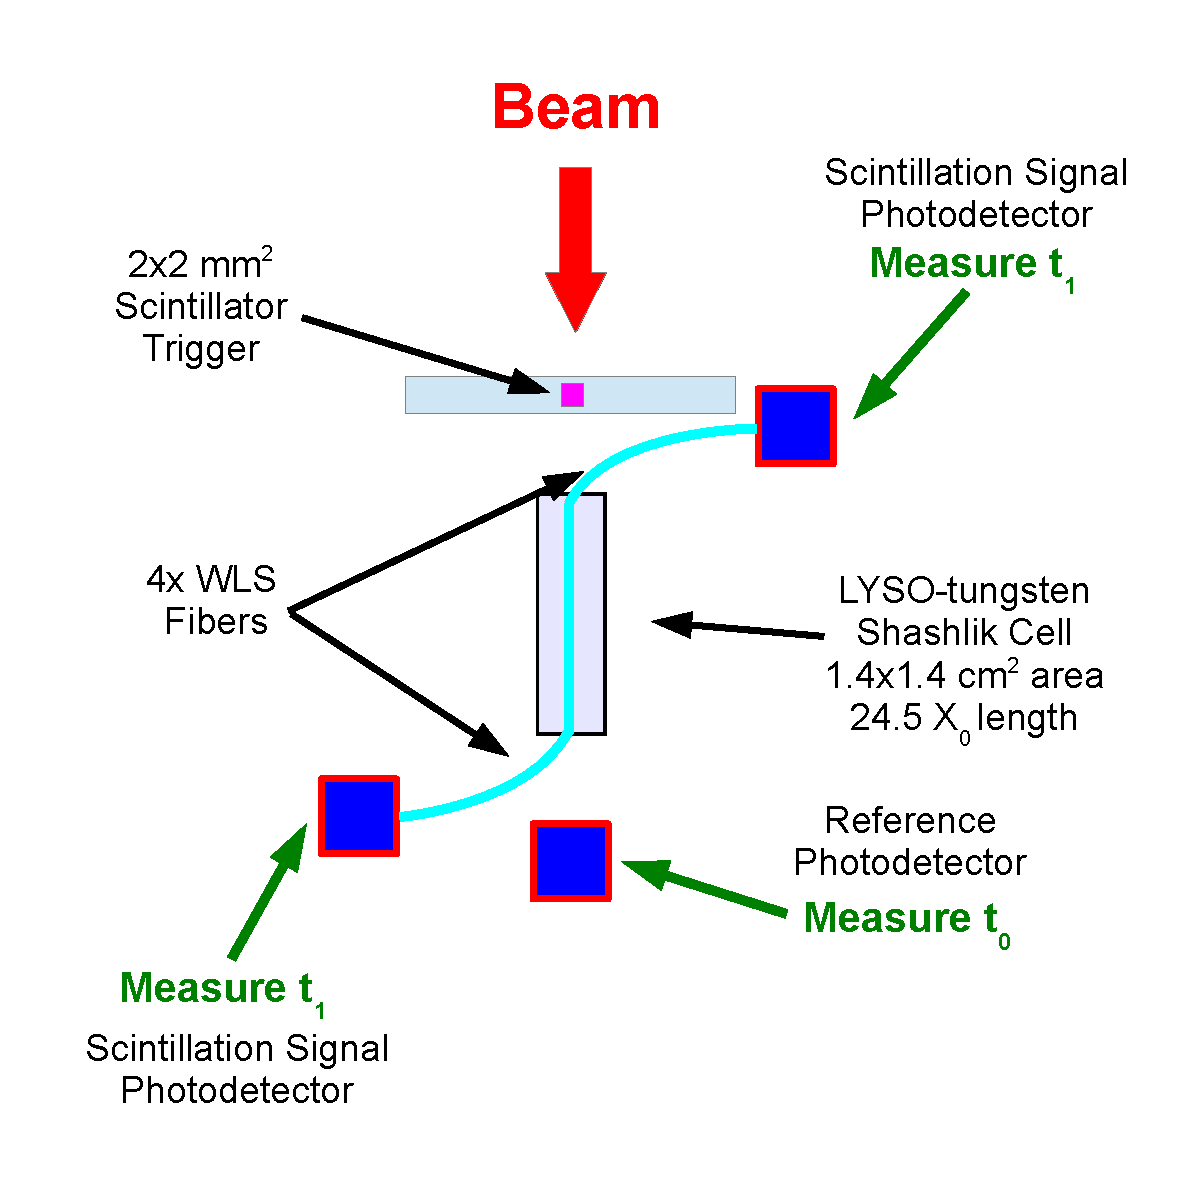
\includegraphics[width=0.45\textwidth]{figs/ShashlikFiberSetupSchematic} 
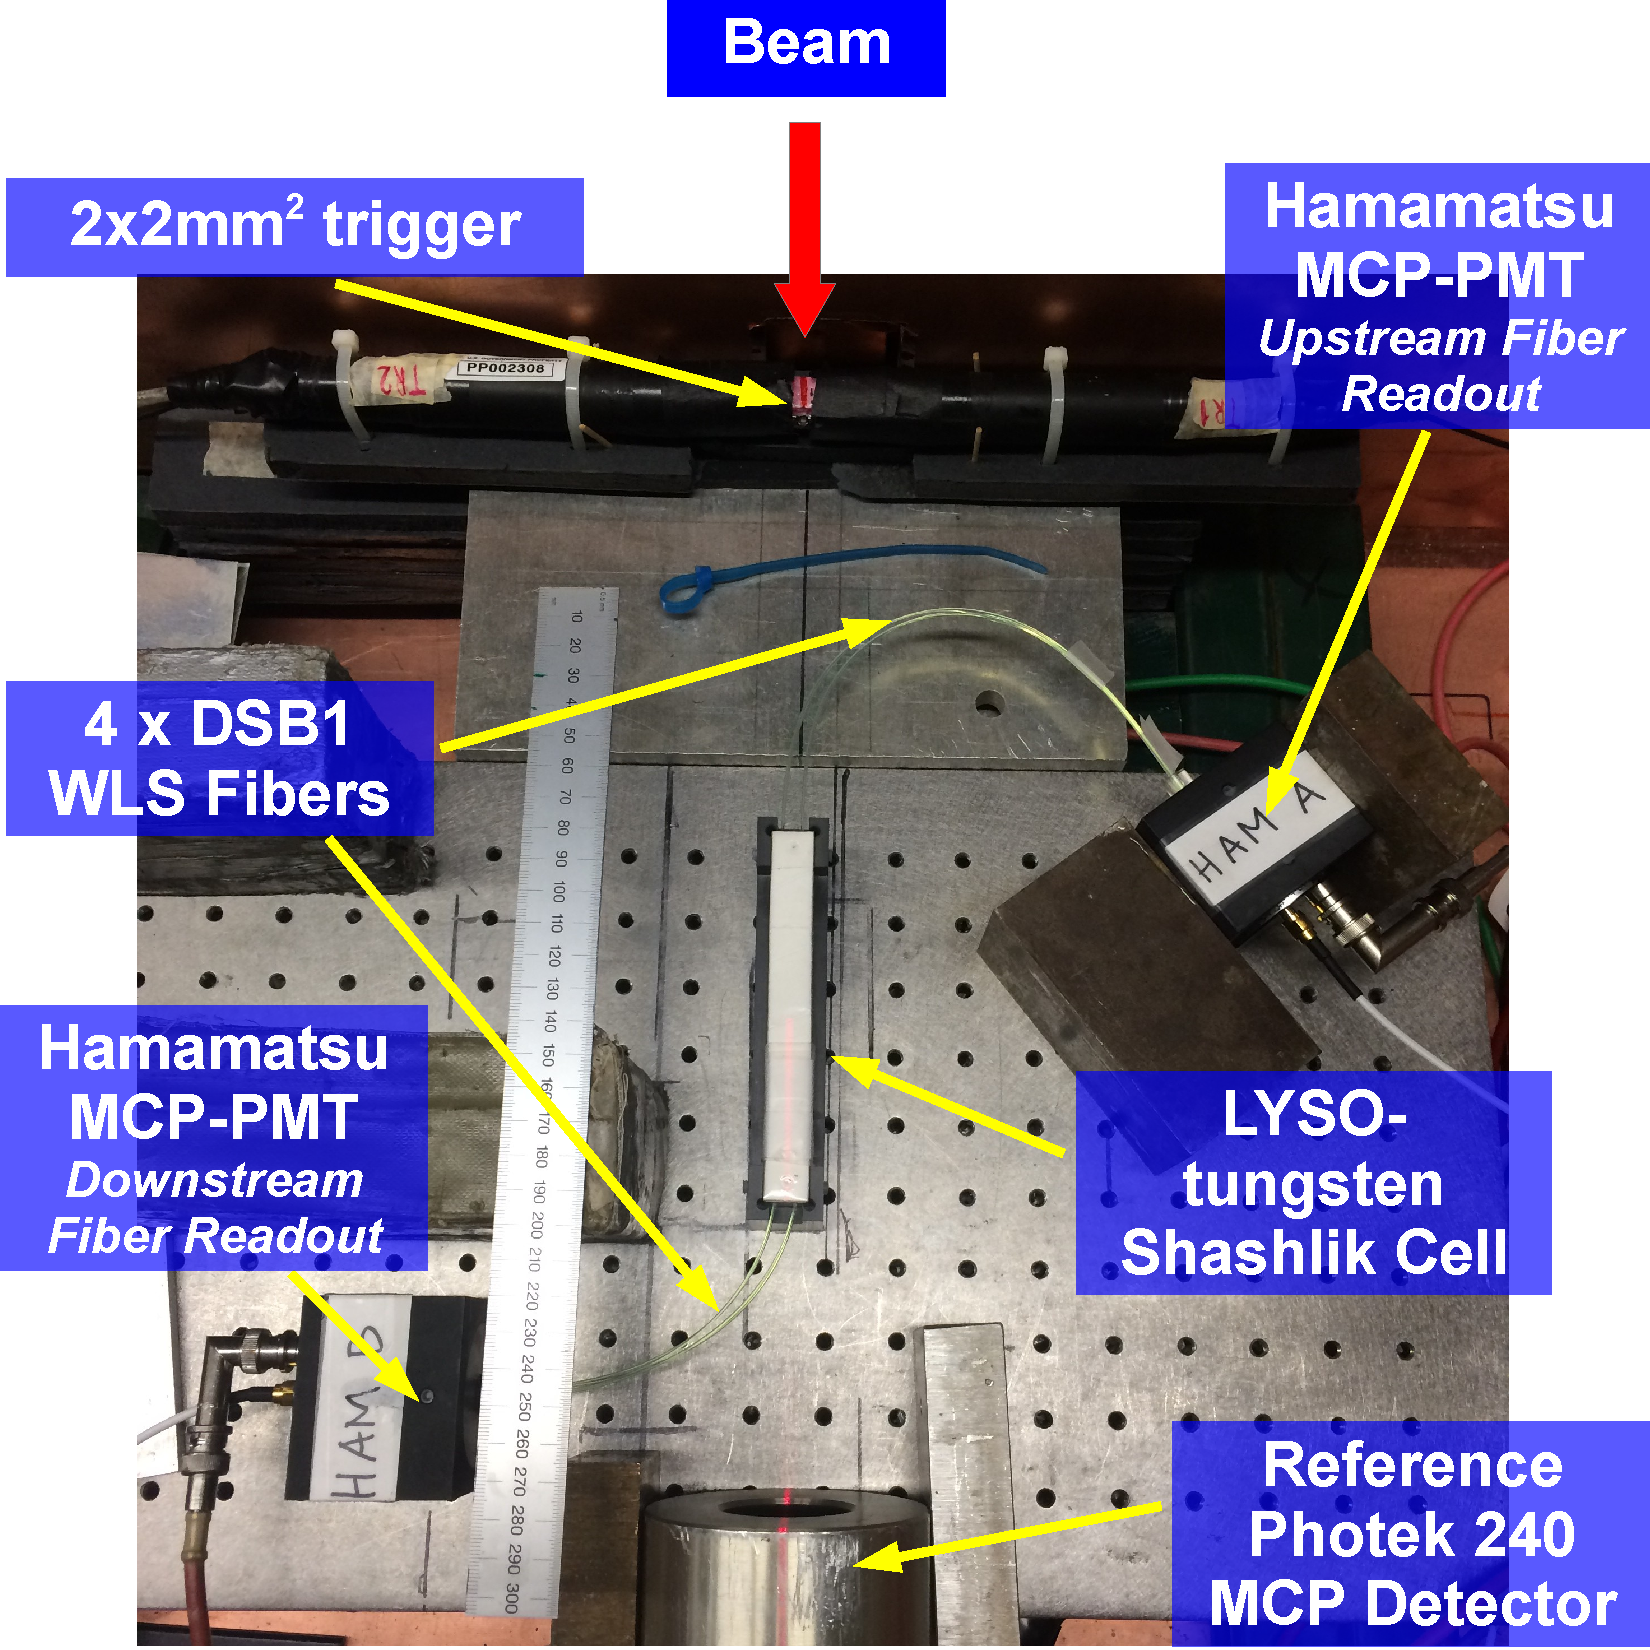
\includegraphics[width=0.45\textwidth]{figs/ShashlikFiberSetupPhoto} 
\caption{ A schematic diagram of the experimental setup for the
time of flight measurement using the LYSO-tungsten shashlik calorimeter
with fiber signal extraction is shown, along with a photograph of the
experimental setup. } 
\label{fig:ShashlikFiberSetup}
\end{figure}

In addition to effects of light transport along the fiber, 
this scheme has the added effect of absorption and re-emission as 
the scintillation light enters the wavelength shifting material. 
The characteristic time scales involved in the wavelength shifting 
mechanism may affect the rise time and time jitter of the final signal 
pulse. We investigate this particular effect in greater detail by
comparing the signal pulses obtained using two different types
of wavelength shifting fiber in the same LYSO-tungsten shashlik
calorimeter. In Figure~\ref{fig:FiberPulseComparison} we show
the pulse shapes averaged over a few hundred events obtained 
using DSB1 fibers and Y11 fibers, plotted in blue and red respectively,
compared with the average pulse shape obtained from direct optical 
coupling of the photodector to the edge of one of the LYSO tiles, plotted in green.
We find that the rise time of the pulse shape obtained using the 
DSB1 fibers, at about $2.4$~ns, is significantly faster than the rise time
of the pulse obtained using the Y11 fibers, which is about $7.1$~ns. This indicates
that the choice of fiber is an important parameter for 
optimizing the time resolution for the design of 
this type of calorimeter, and that the DSB1 fiber 
already provides a reasonably good choice.

\begin{figure}[H] \centering
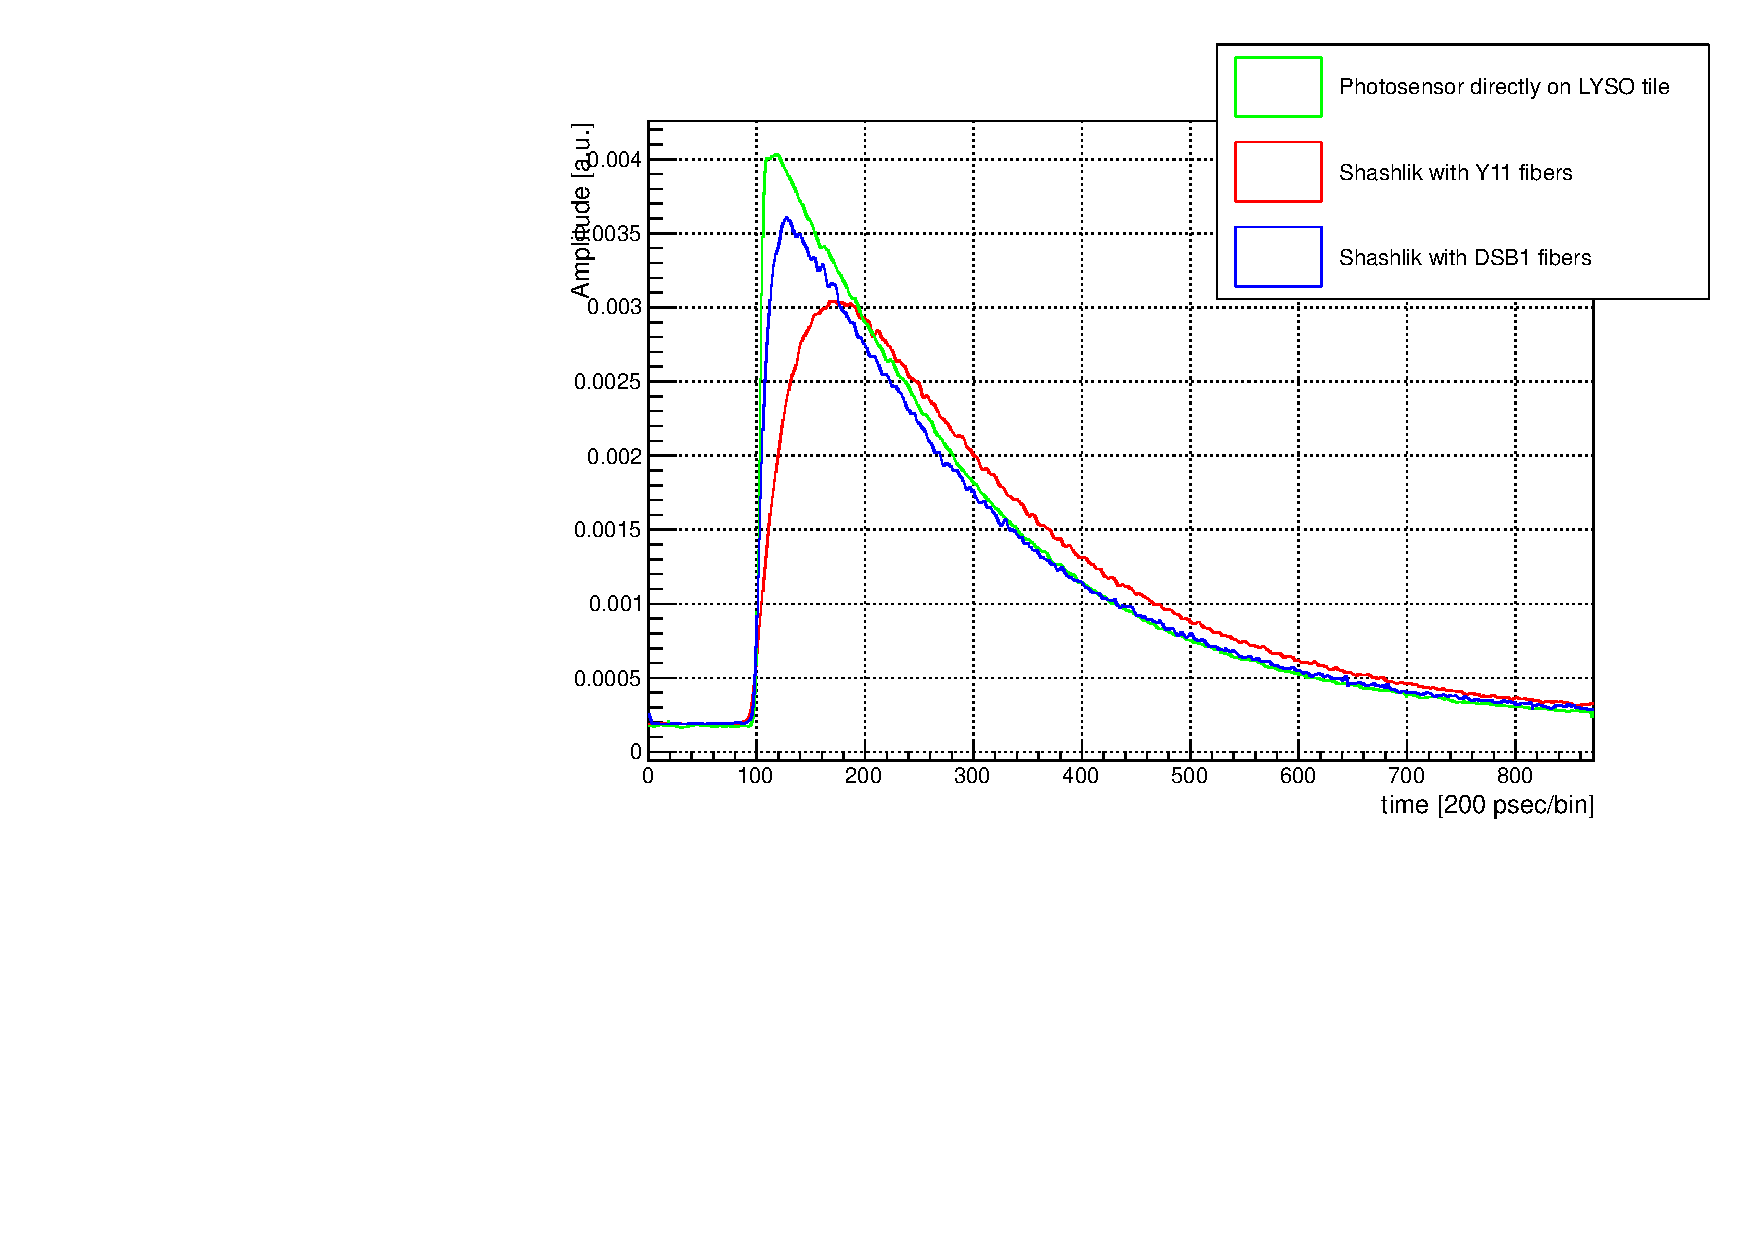
\includegraphics[width=0.45\textwidth]{figs/FiberPulses} 
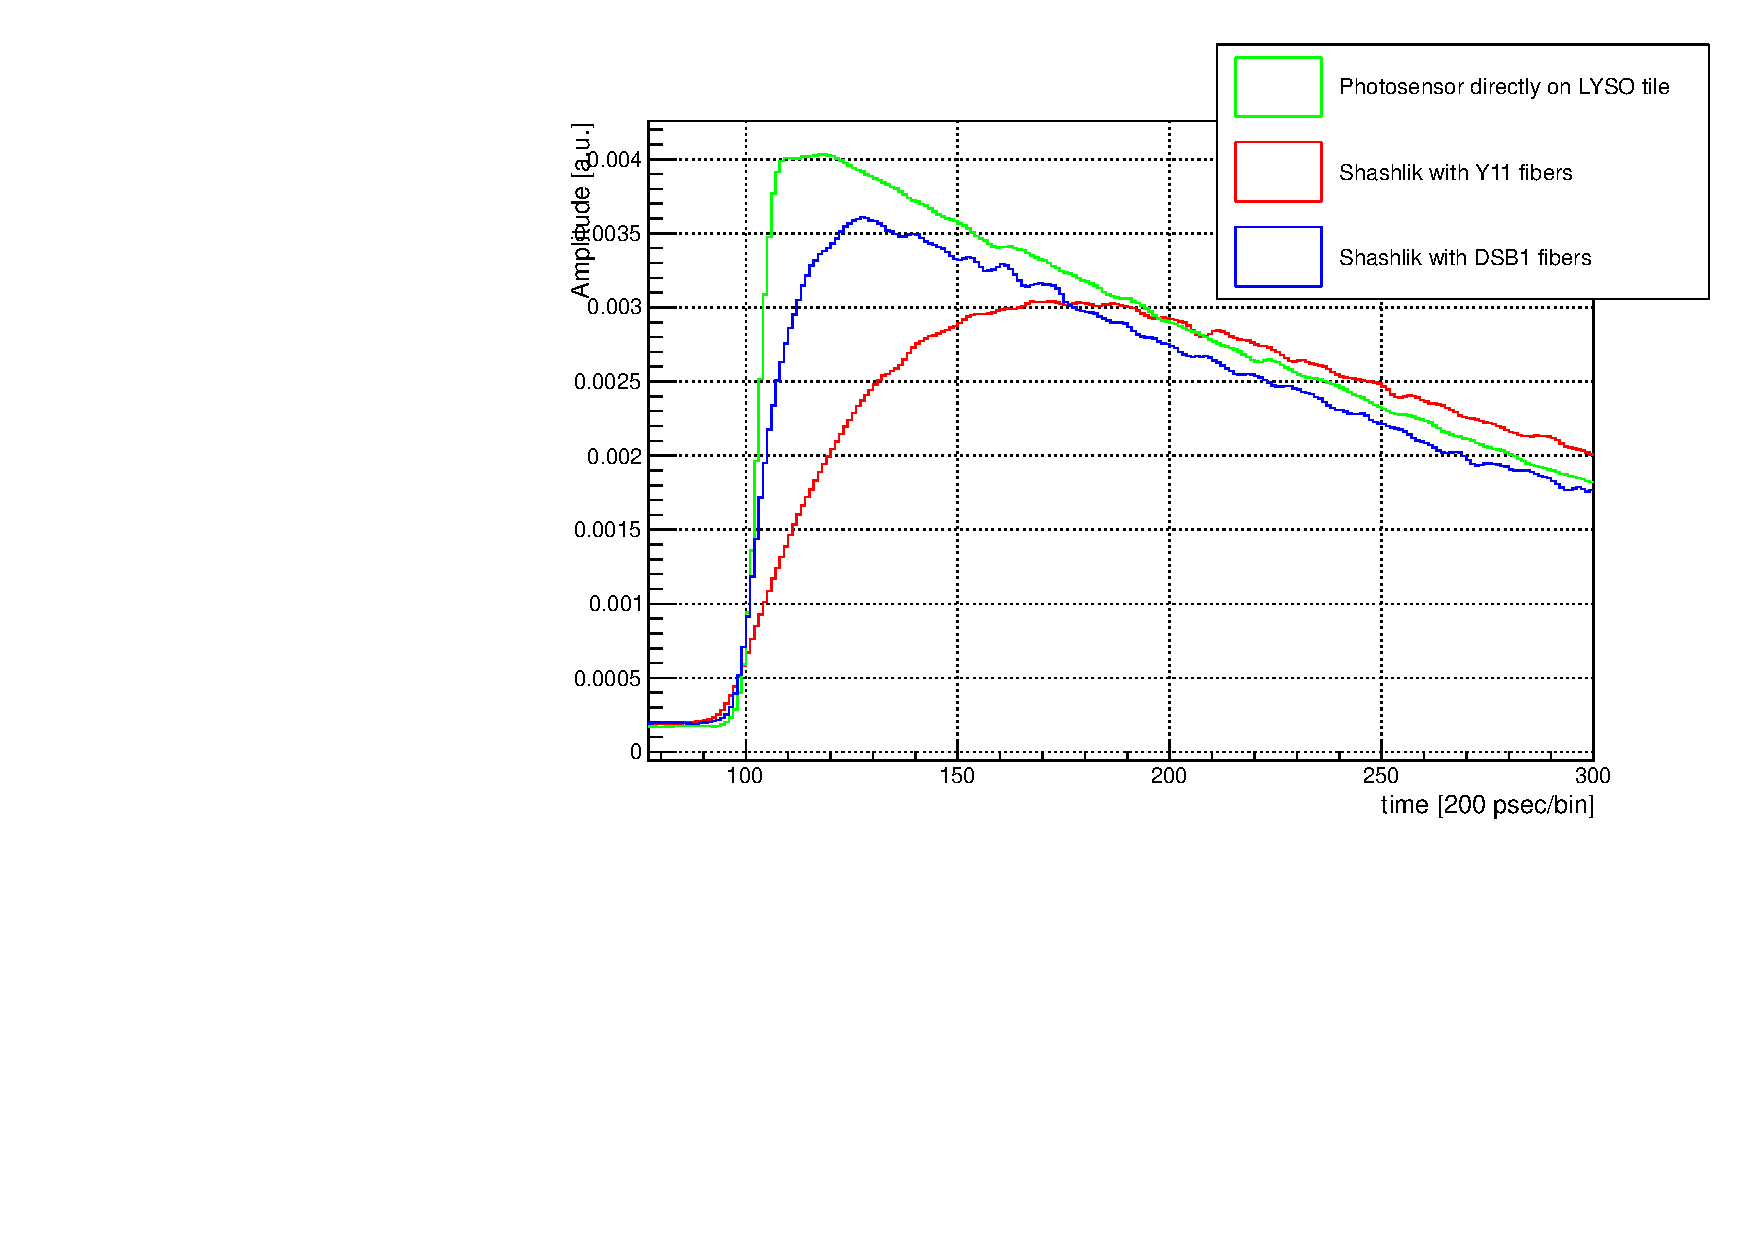
\includegraphics[width=0.45\textwidth]{figs/FiberPulsesZoom} 
\caption{(Left) Pulse shapes digitized by the DRS4 board and averaged over several hundred events 
obtained from the LYSO-tungsten shashlik calorimeter with light extracted using
DSB1 (blue) and Y11 (red) wavelength shifting fibers, are compared with 
the averaged pulse shapes obtained from direct coupling of the photodetector (green)
to one edge of one of the LYSO tiles in the shashlik calorimeter. (Right) A zoomed-in version of the figure on the left.} 
\label{fig:FiberPulseComparison}
\end{figure}


Using the DSB1 fibers, we measure the time resolution
for electron beams with beam energy varying between $4$~GeV and $32$~GeV.
In Figure~\ref{fig:ShashlikFiberEnergy32GeV} we show the distribution
of the pulse integral, a quantity proportional to the total collected charge,
for the $32$~GeV beam and observe an energy resolution of about $5\%$.
The time of flight distributions, fitted to gaussian functions,
are shown in Figure~\ref{fig:ShashlikFiberTOF}, and the resulting
$\sigma$ parameter of the gaussian is plotted as a function of the
beam energy in Figure~\ref{fig:ShashlikFiberTOFResolutionVsEnergy}.
We find that the dependence of the time resolution on
beam energy exhibits a $1/\sqrt{E}$ functional form, indicating
that the current calorimeter setup remains in the photo-statistics
limited regime. The best time resolution we obtain
with this setup is $104$~ps. As the measurement is photo-statistics
limited, to improve on this result in the future, work is needed
on improving the light collection efficiency. 

\begin{figure}[H] \centering
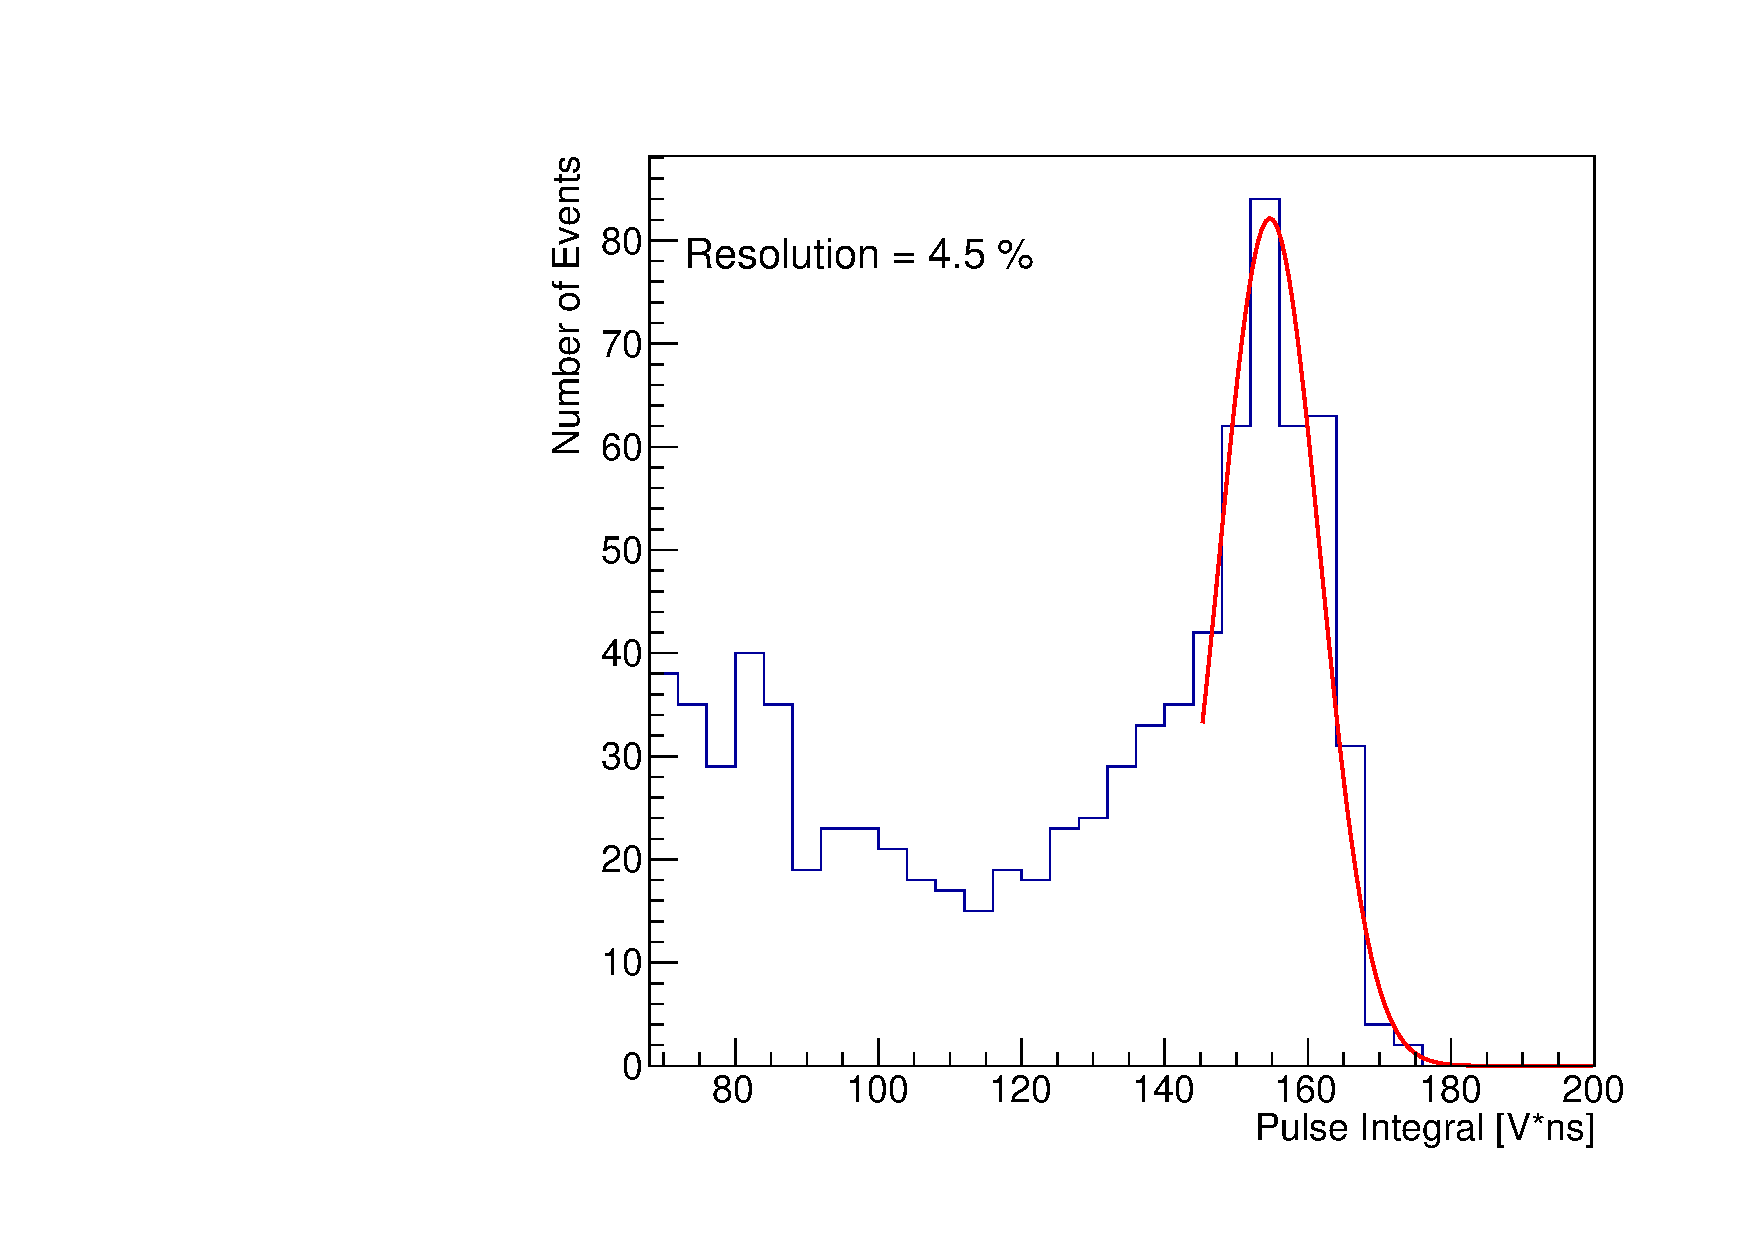
\includegraphics[width=0.45\textwidth]{figs/TOF_ShashlikDSB1Fiber_Electron_32GeV_energy} 
\caption{ Histogram of the pulse integral for events recorded using
the LYSO-tungsten shashlik calorimeter using the DSB1 fibers for 
a $32$~GeV electron beam. No electron identification requirements
are made for this run due to a misconfiguration of the Cherenkov counter
and background is visible in the spectrum as a result. } 
\label{fig:ShashlikFiberEnergy32GeV}
\end{figure}

\begin{figure}[H] \centering
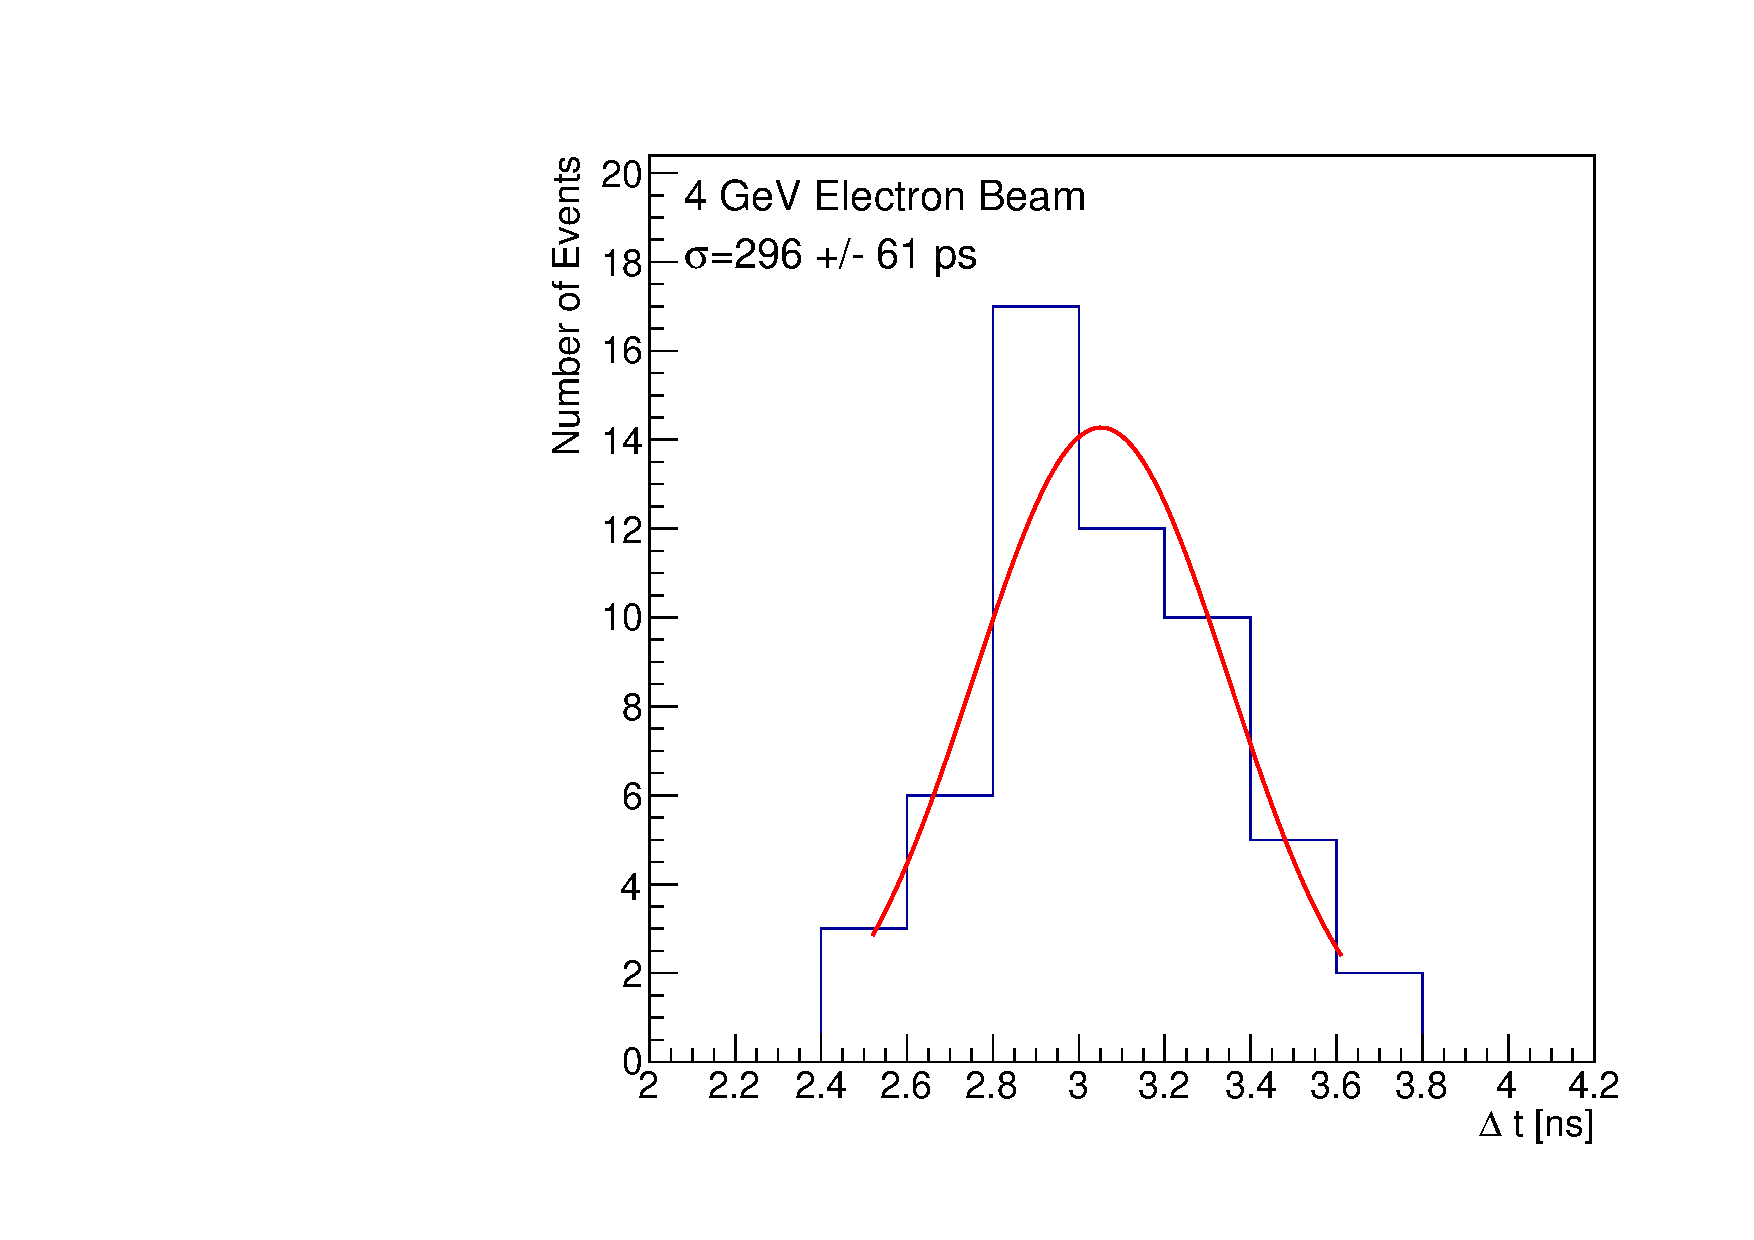
\includegraphics[width=0.45\textwidth]{figs/TOF_ShashlikDSB1Fiber_Electron_4GeV} 
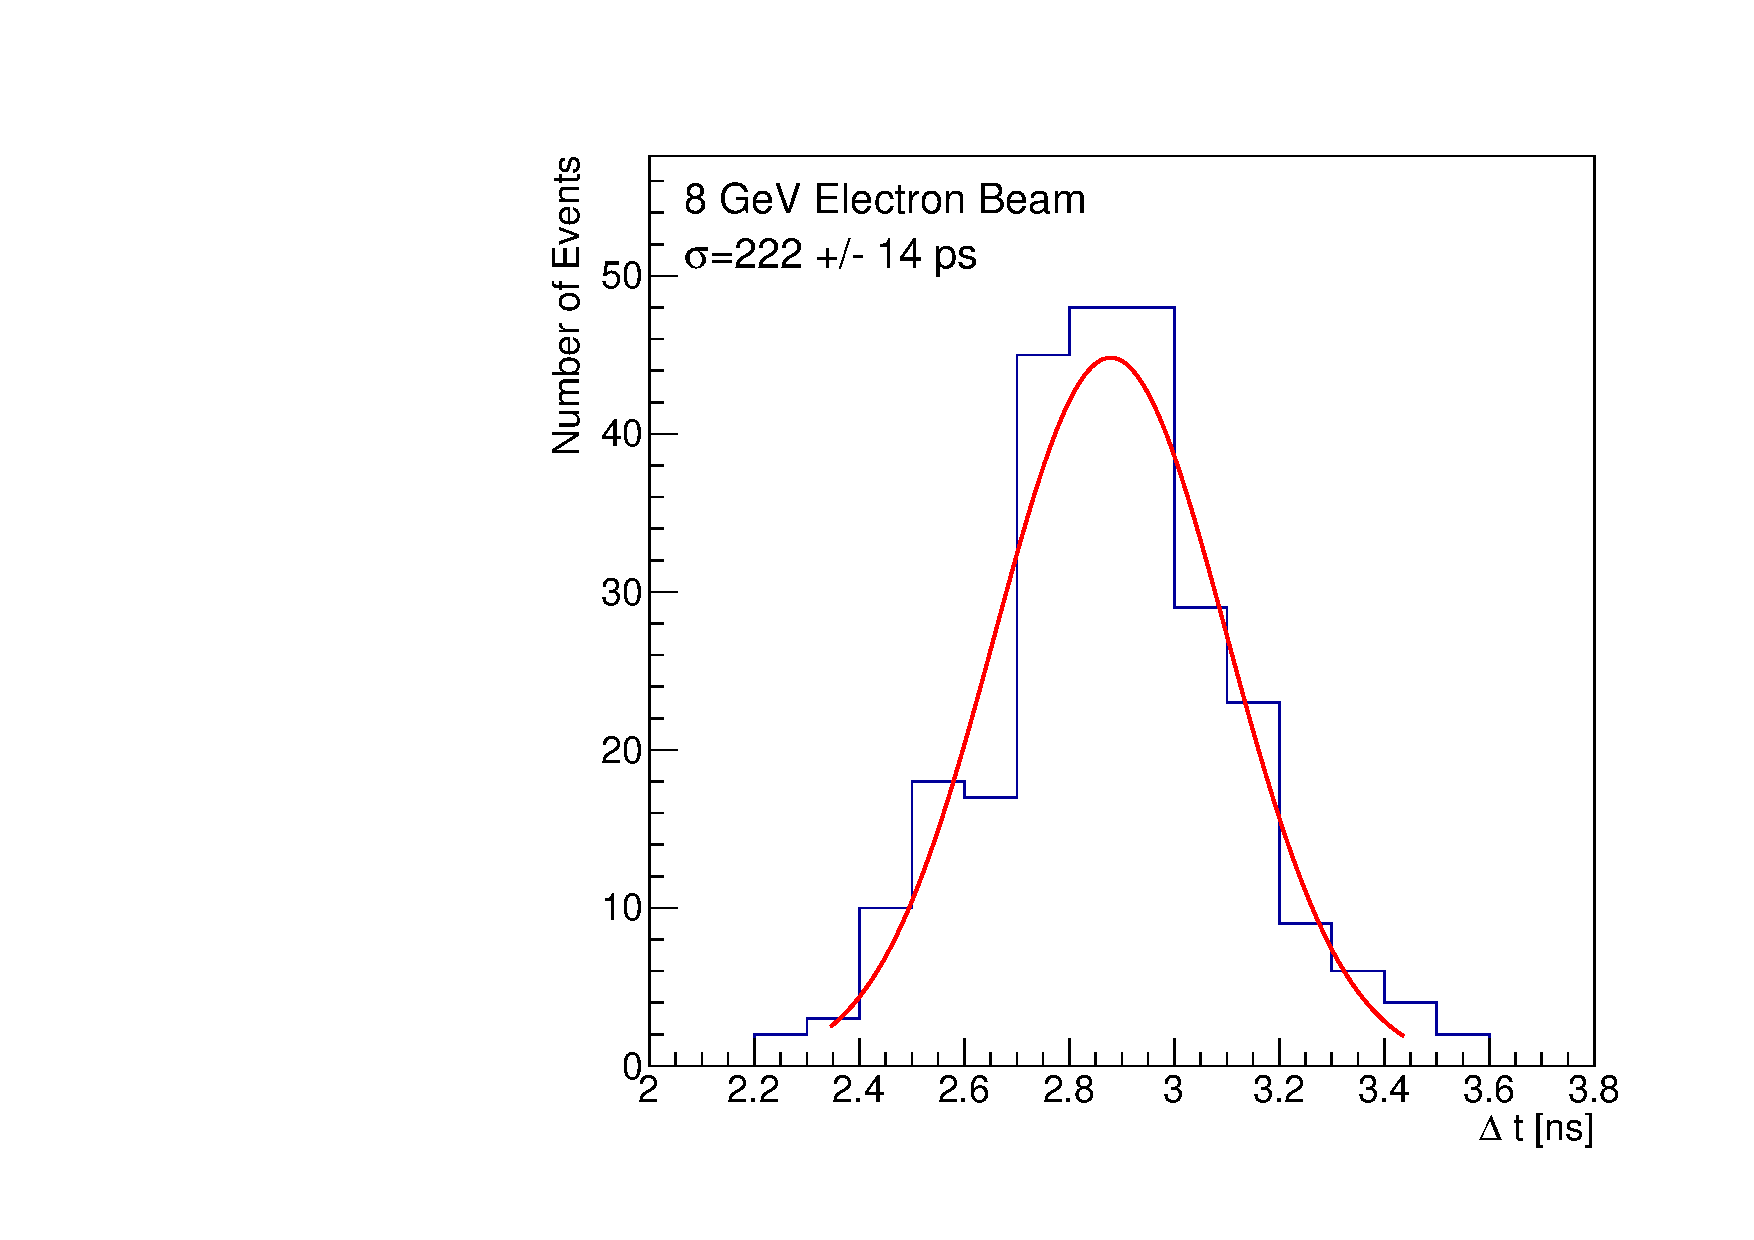
\includegraphics[width=0.45\textwidth]{figs/TOF_ShashlikDSB1Fiber_Electron_8GeV} 
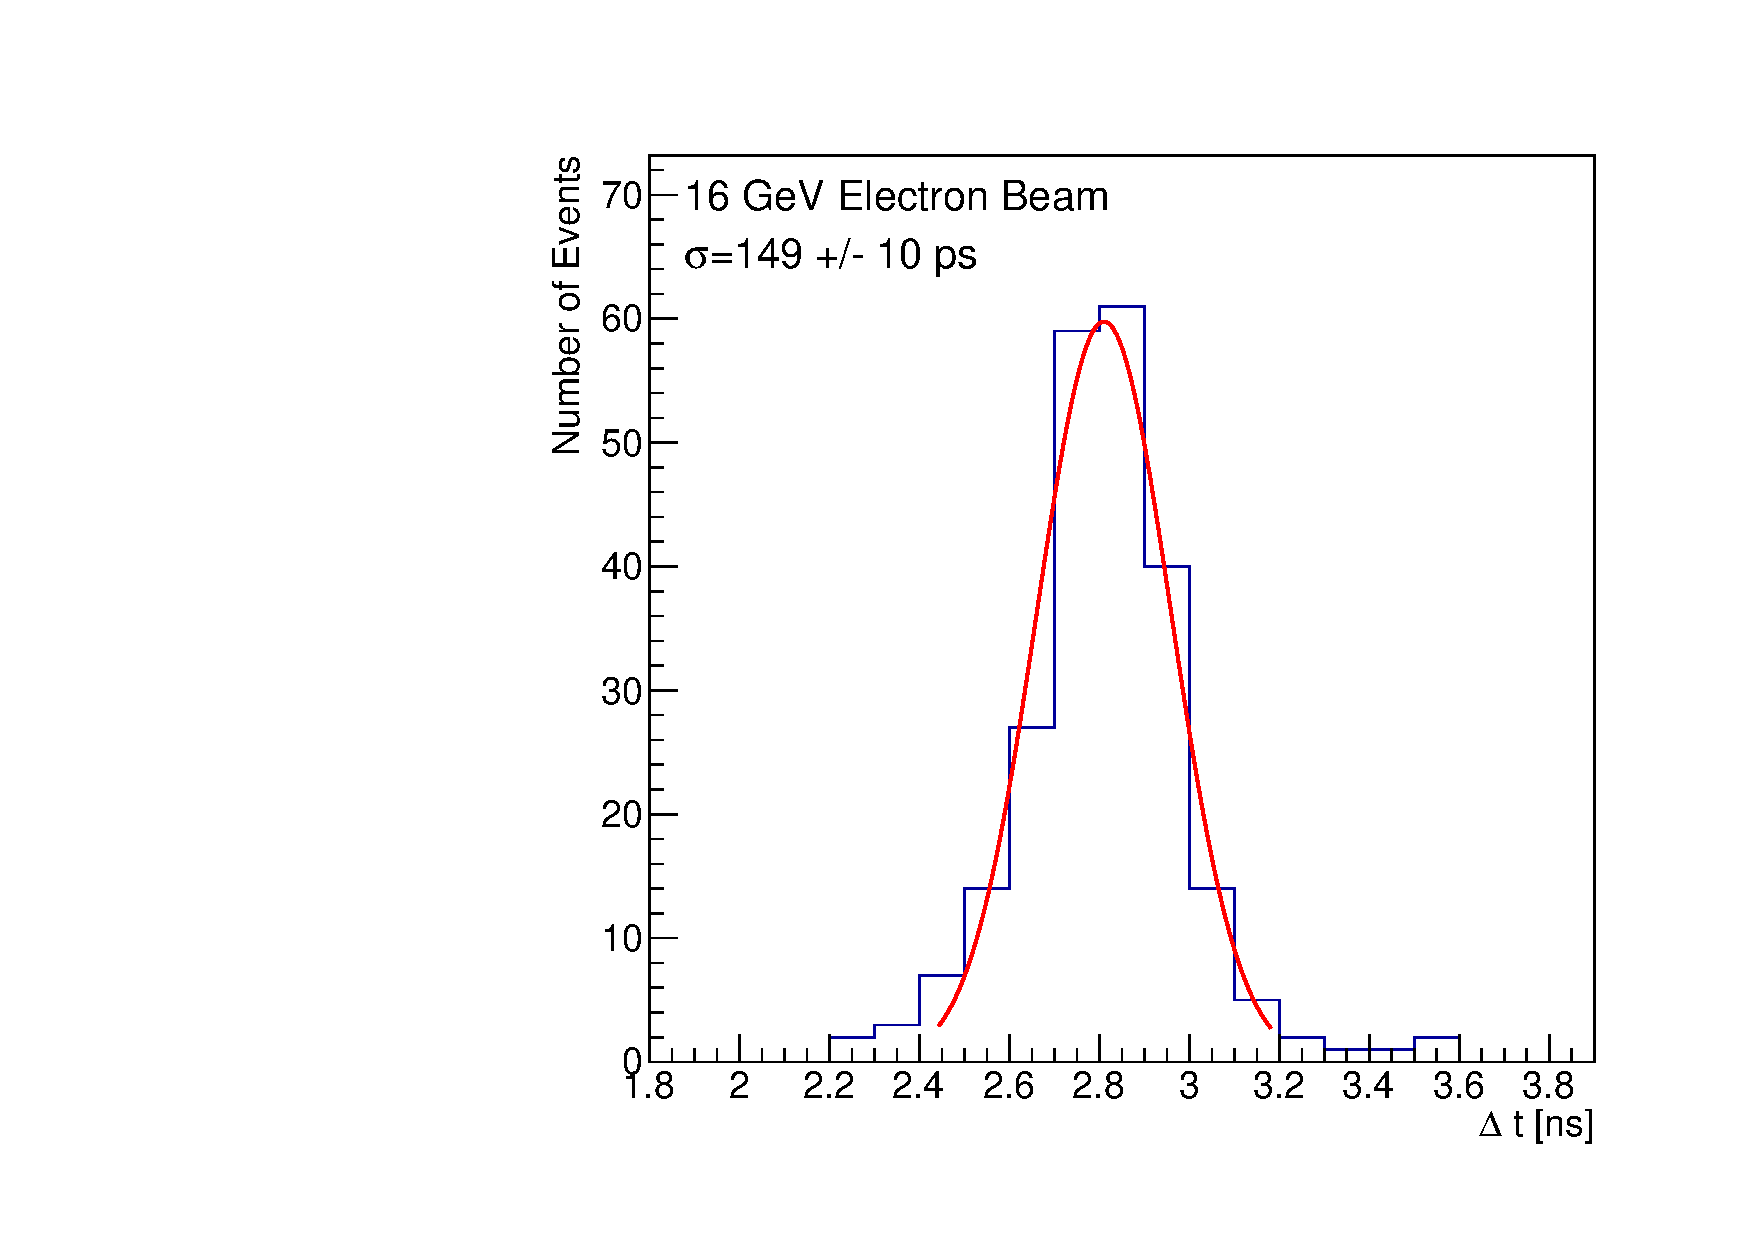
\includegraphics[width=0.45\textwidth]{figs/TOF_ShashlikDSB1Fiber_Electron_16GeV} 
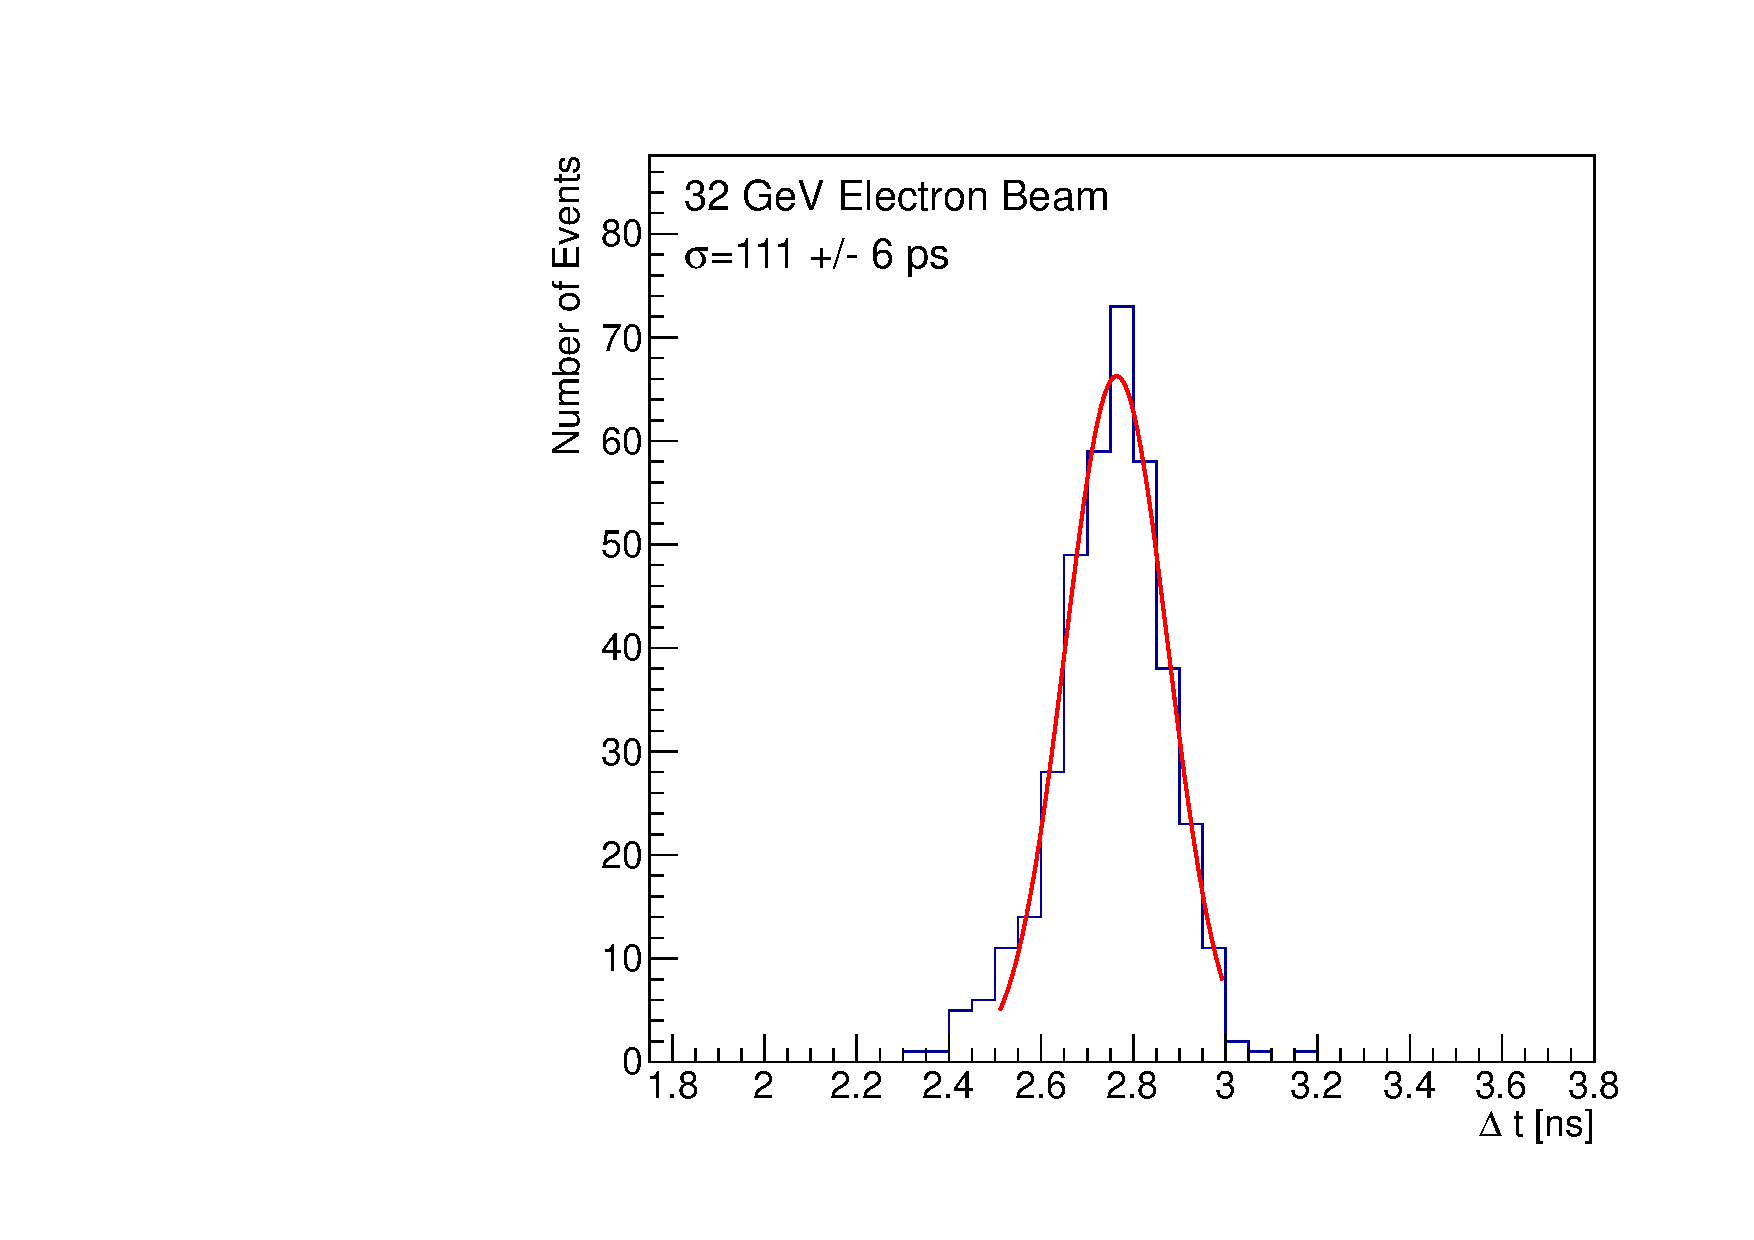
\includegraphics[width=0.45\textwidth]{figs/TOF_ShashlikDSB1Fiber_Electron_32GeV} 
\caption{ Time of flight distributions for the LYSO-tungsten shashlik calorimeter
using DSB1 fibers for electron beams with varying beam energies. } 
\label{fig:ShashlikFiberTOF}
\end{figure}

\begin{figure}[H] \centering
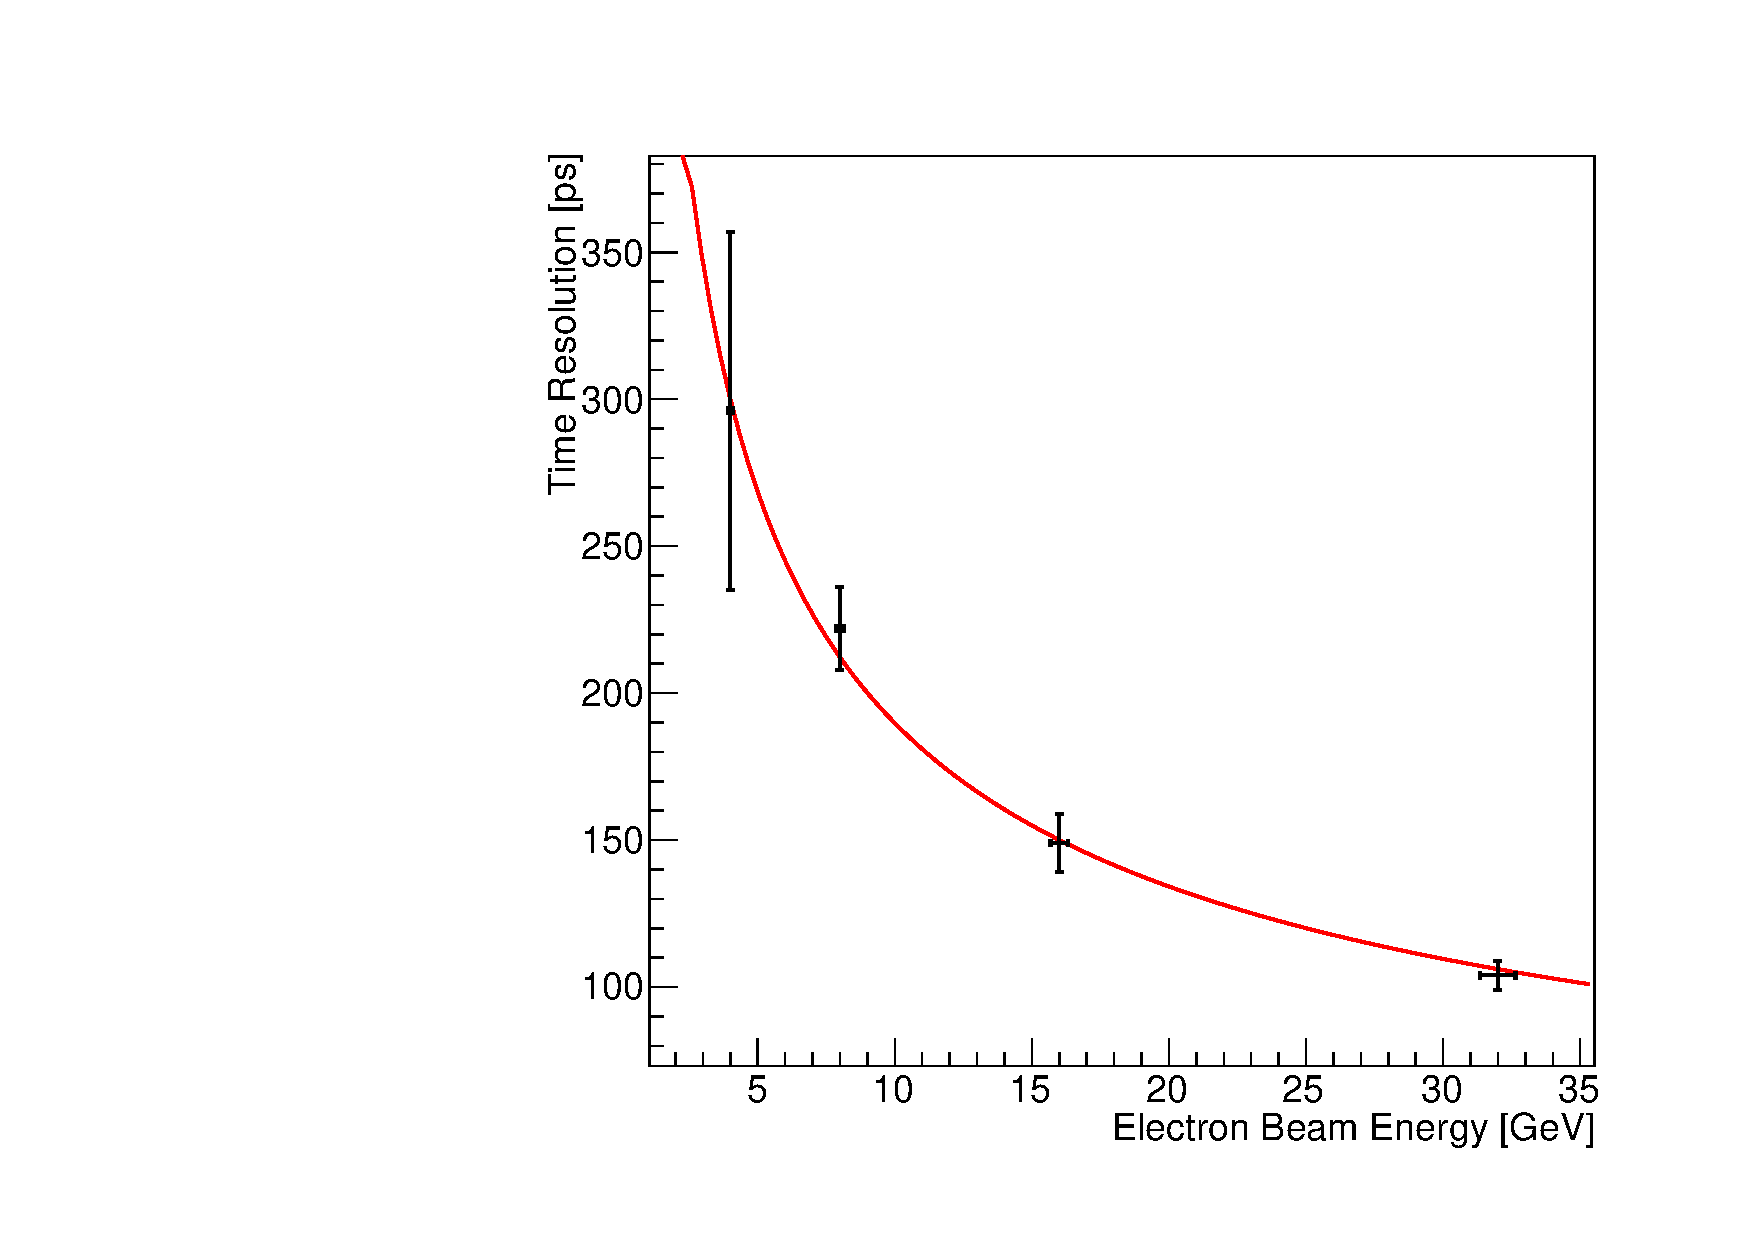
\includegraphics[width=0.45\textwidth]{figs/TimeResolutionVsEnergy_ShashlikDSB1Fiber} 
\caption{ The time resolution measured using the LYSO-tungsten shashlik
calorimeter with signal extracted using DSB1 fibers is plotted as a function of
the electron beam energy, and fitted to a $1/\sqrt{E}$ functional form. }
\label{fig:ShashlikFiberTOFResolutionVsEnergy}
\end{figure}


Next, we studied an alternative scheme where the MCP-PMT photodetectors
are directly coupled to the edge of two subsequent LYSO layers of the
shashlik calorimeter and scintillation light is directly transported 
to the photodetector through the edge of the tile layers. 
A schematic diagram and corresponding photograph of
the experimental setup is shown in Figure~\ref{fig:ShashlikSideReadoutSetup}.
In Figure~\ref{fig:ShashlikSideReadoutExposedLayersPhoto}, we show
a zoomed in photograph of the exposed LYSO layers, from which the 
scintillation light signal is extracted.

\begin{figure}[H] \centering
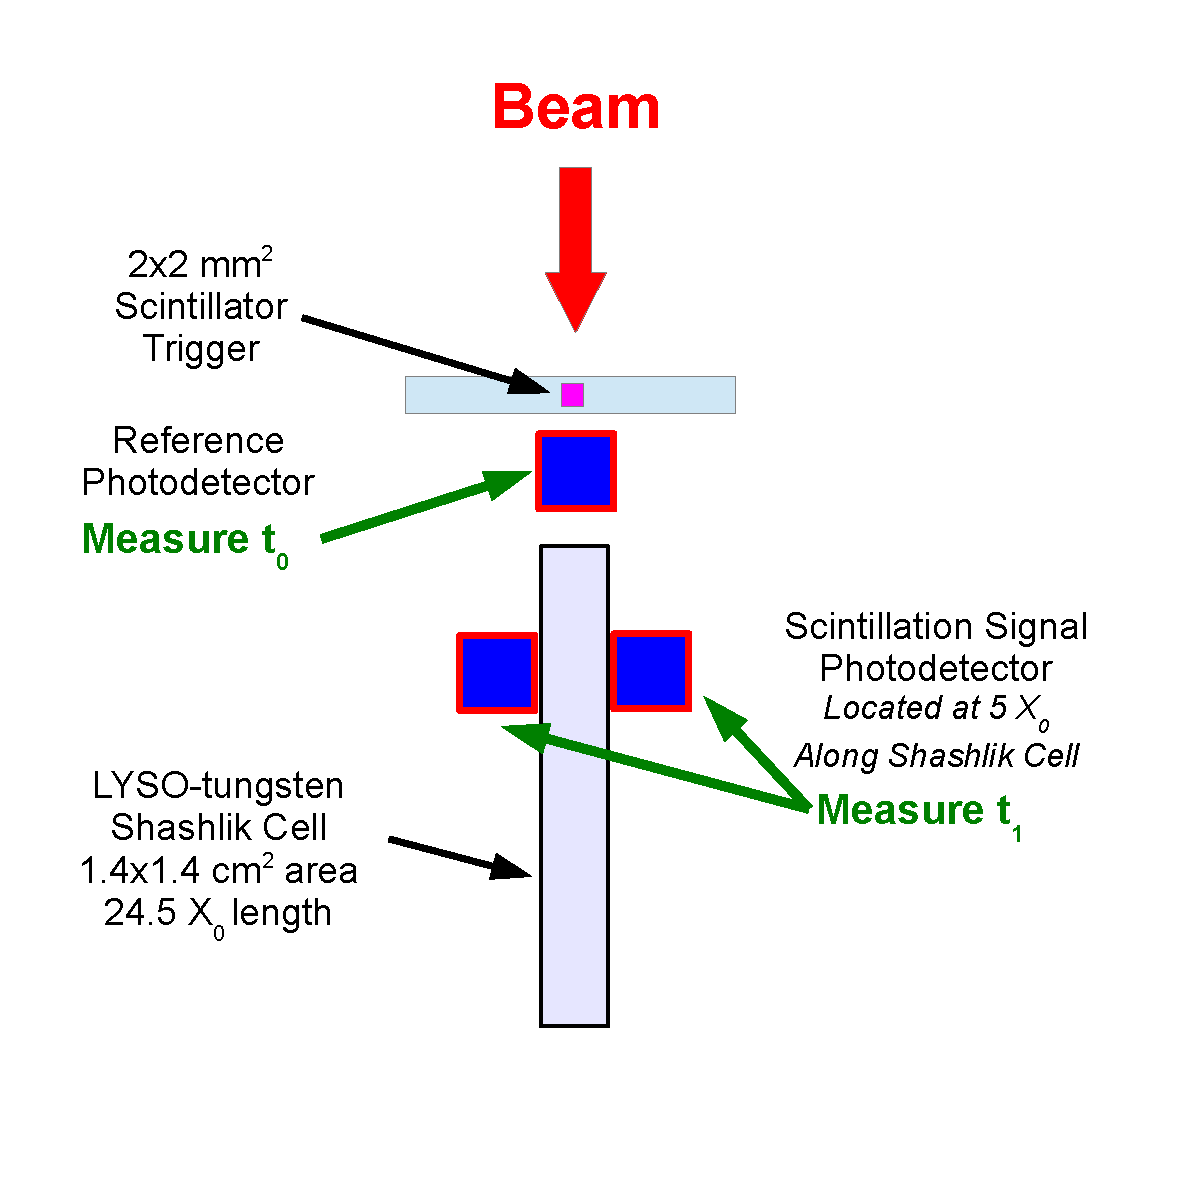
\includegraphics[width=0.45\textwidth]{figs/ShashlikSideReadoutSetupSchematic} 
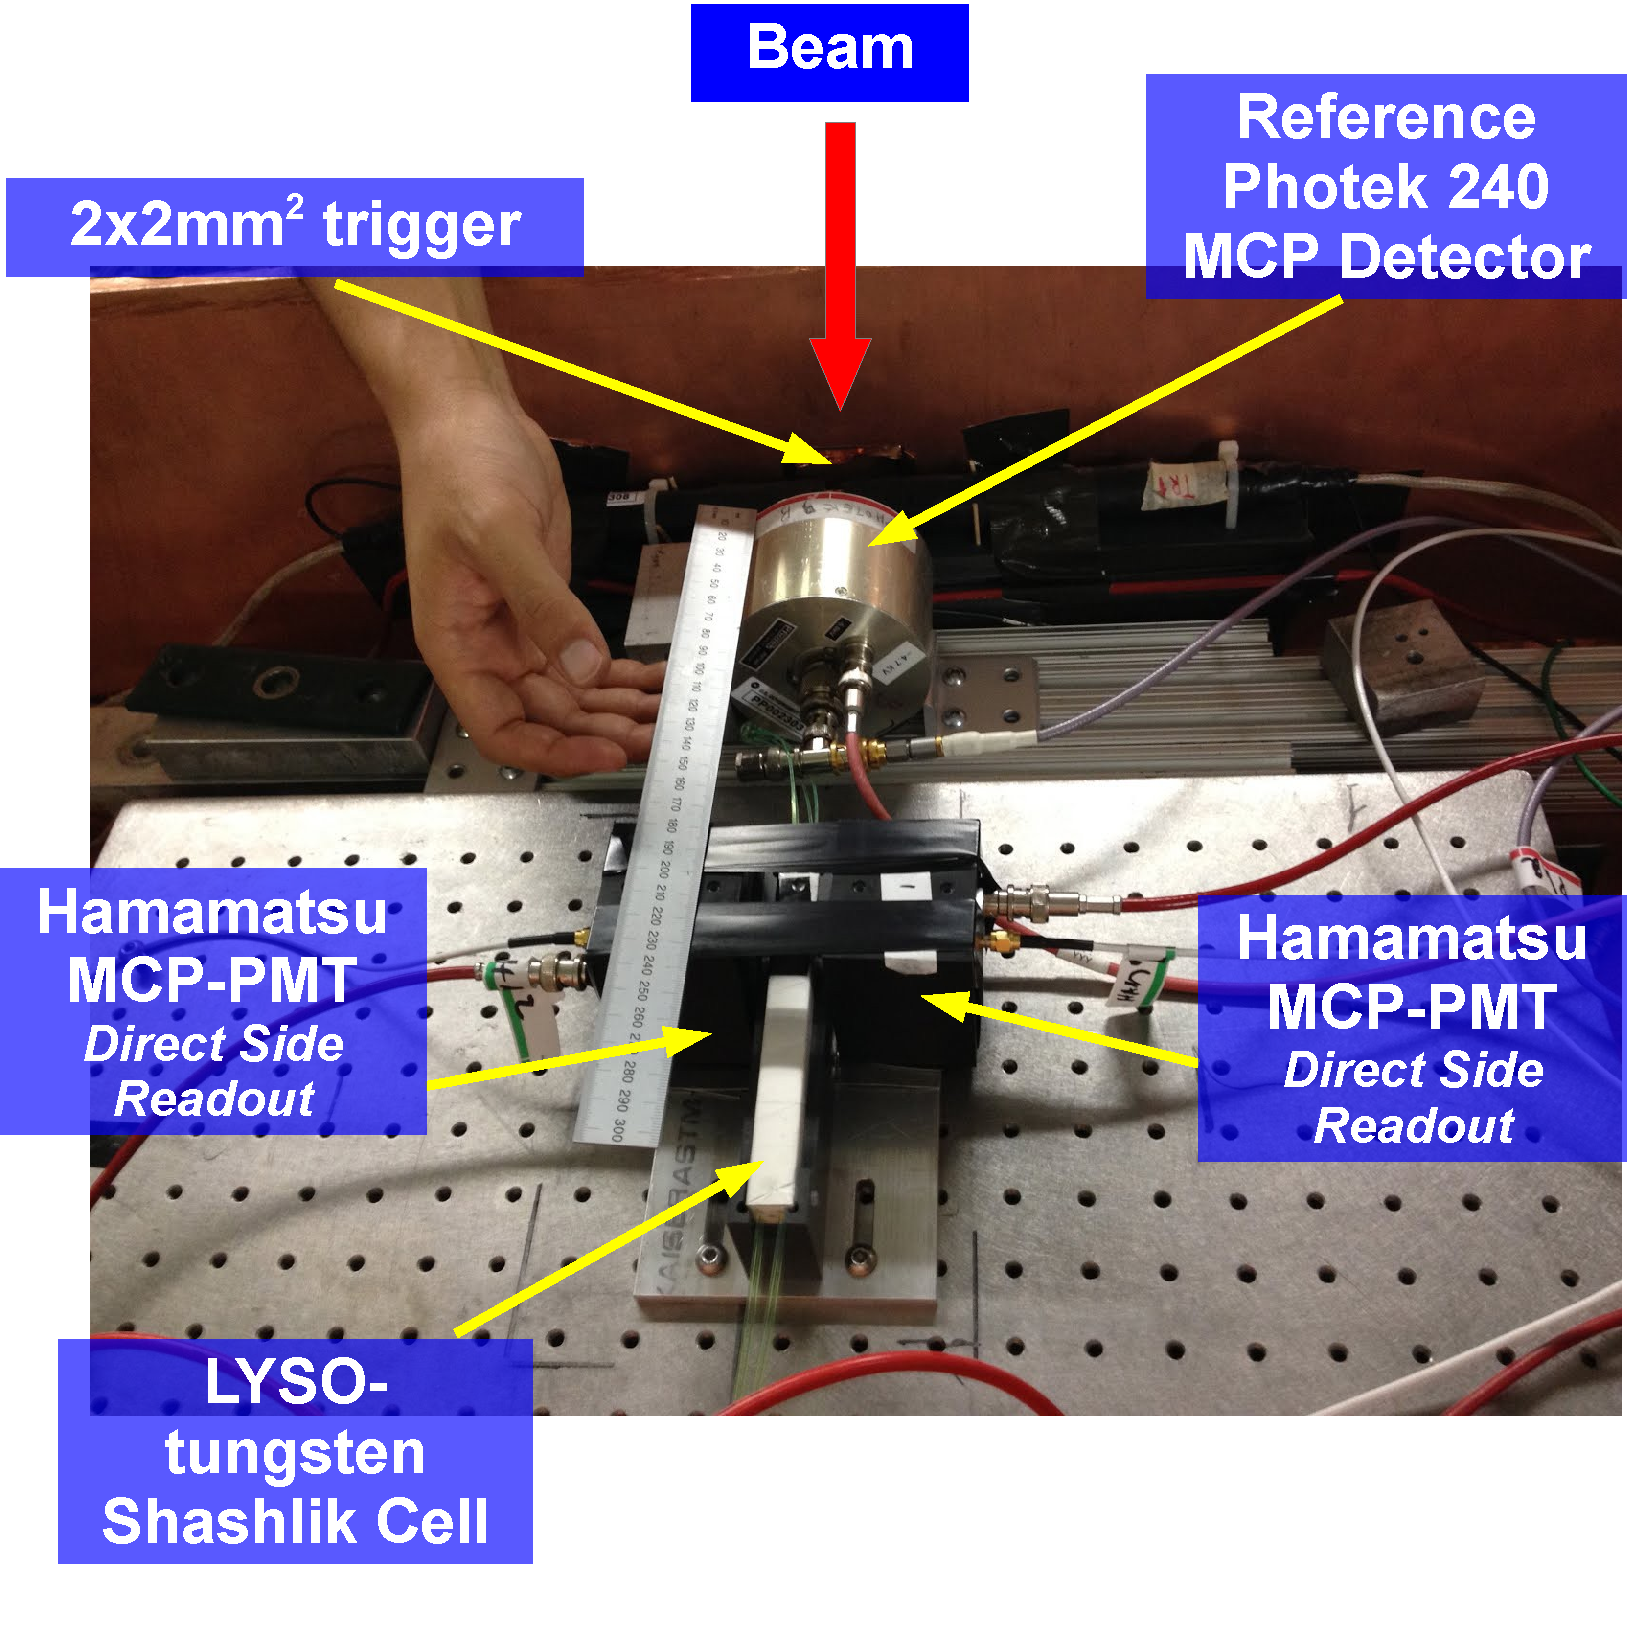
\includegraphics[width=0.45\textwidth]{figs/ShashlikSideReadoutPhotoB} 
\caption{ A schematic diagram of the experimental setup for the
time of flight measurement using the LYSO-tungsten shashlik calorimeter
with signal extraction from the edges of two LYSO layers is shown, along
with a photograph of the experimental setup. } 
\label{fig:ShashlikSideReadoutSetup}
\end{figure}

\begin{figure}[H] \centering
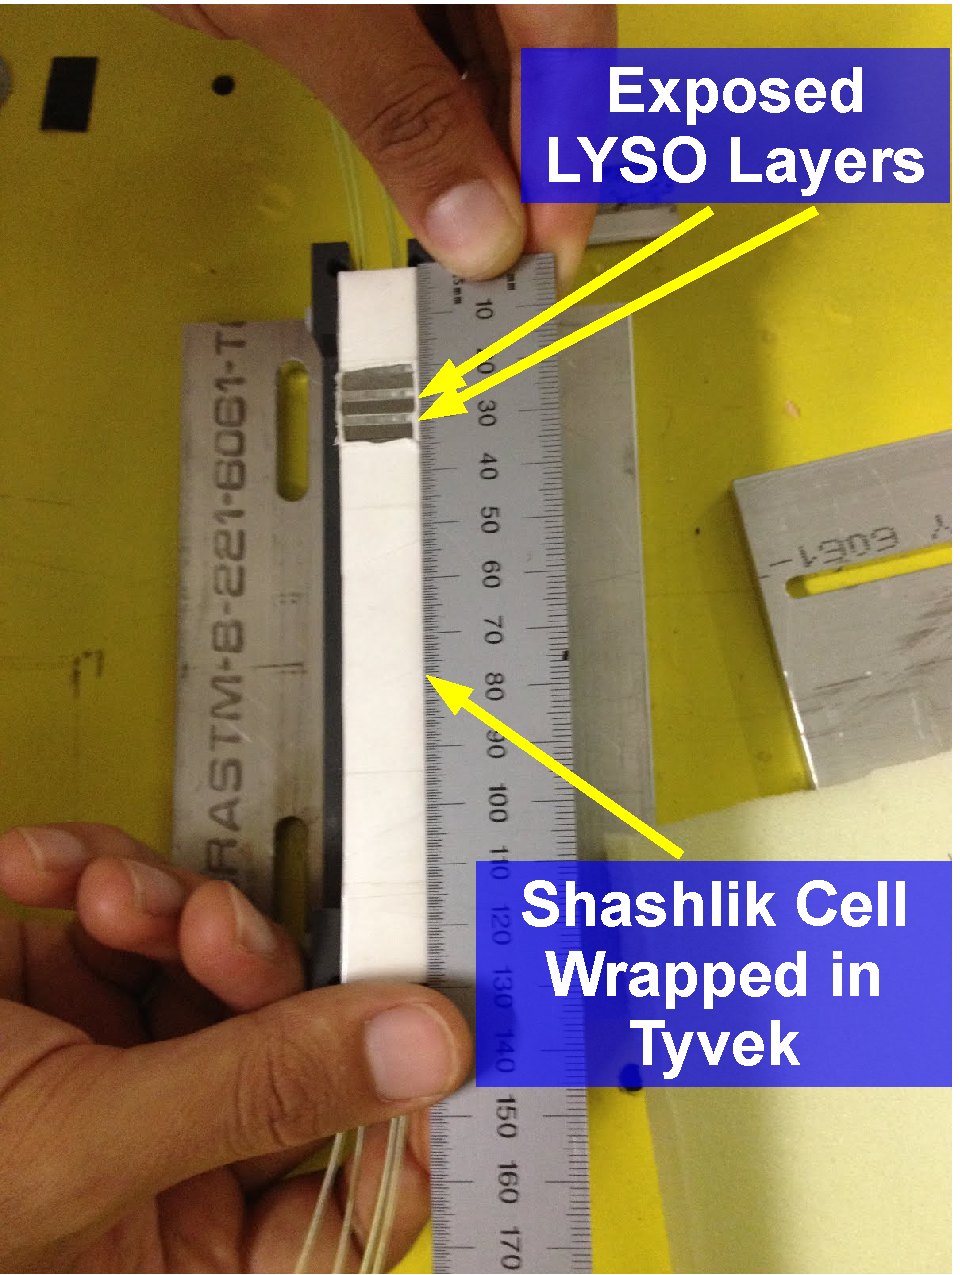
\includegraphics[width=0.30\textwidth]{figs/ShashlikSideReadoutPhotoA} 
\caption{ A photograph of the two exposed LYSO layers is shown.
The scintillation light signal is extracted by optically coupling
the edges of these two exposed LYSO layers to the MCP-PMT
photodetectors. } 
\label{fig:ShashlikSideReadoutExposedLayersPhoto}
\end{figure}

With the intention to study the relationship between the impact of the 
optical transit time jitter and the impact of limited photo-statistics,
we minimize the distance that the scintillation light
must travel to reach the photodetector in this setup and thereby minimize the
impact of optical transit on the time resolution but reduce the photostatistics 
as we collect light from only a fraction of the edges of two LYSO layers. 
In Figure~\ref{fig:ShashlikSideReadoutTOF}, we show the 
time of flight distributions for electron beams at various energies, 
fitted to gaussian functions. The resulting
$\sigma$ parameter of the gaussian is plotted as a function of the
beam energy in Figure~\ref{fig:ShashlikSideReadoutTOFResolutionVsEnergy}.
The best time  resolution that we obtain is about $55$~ps, and
fitting the result to the sum of a $1/\sqrt{E}$ term and a constant term,
we find a constant term of about $30$~ps with a statistical uncertainty of $30\%$. 

\begin{figure}[H] \centering
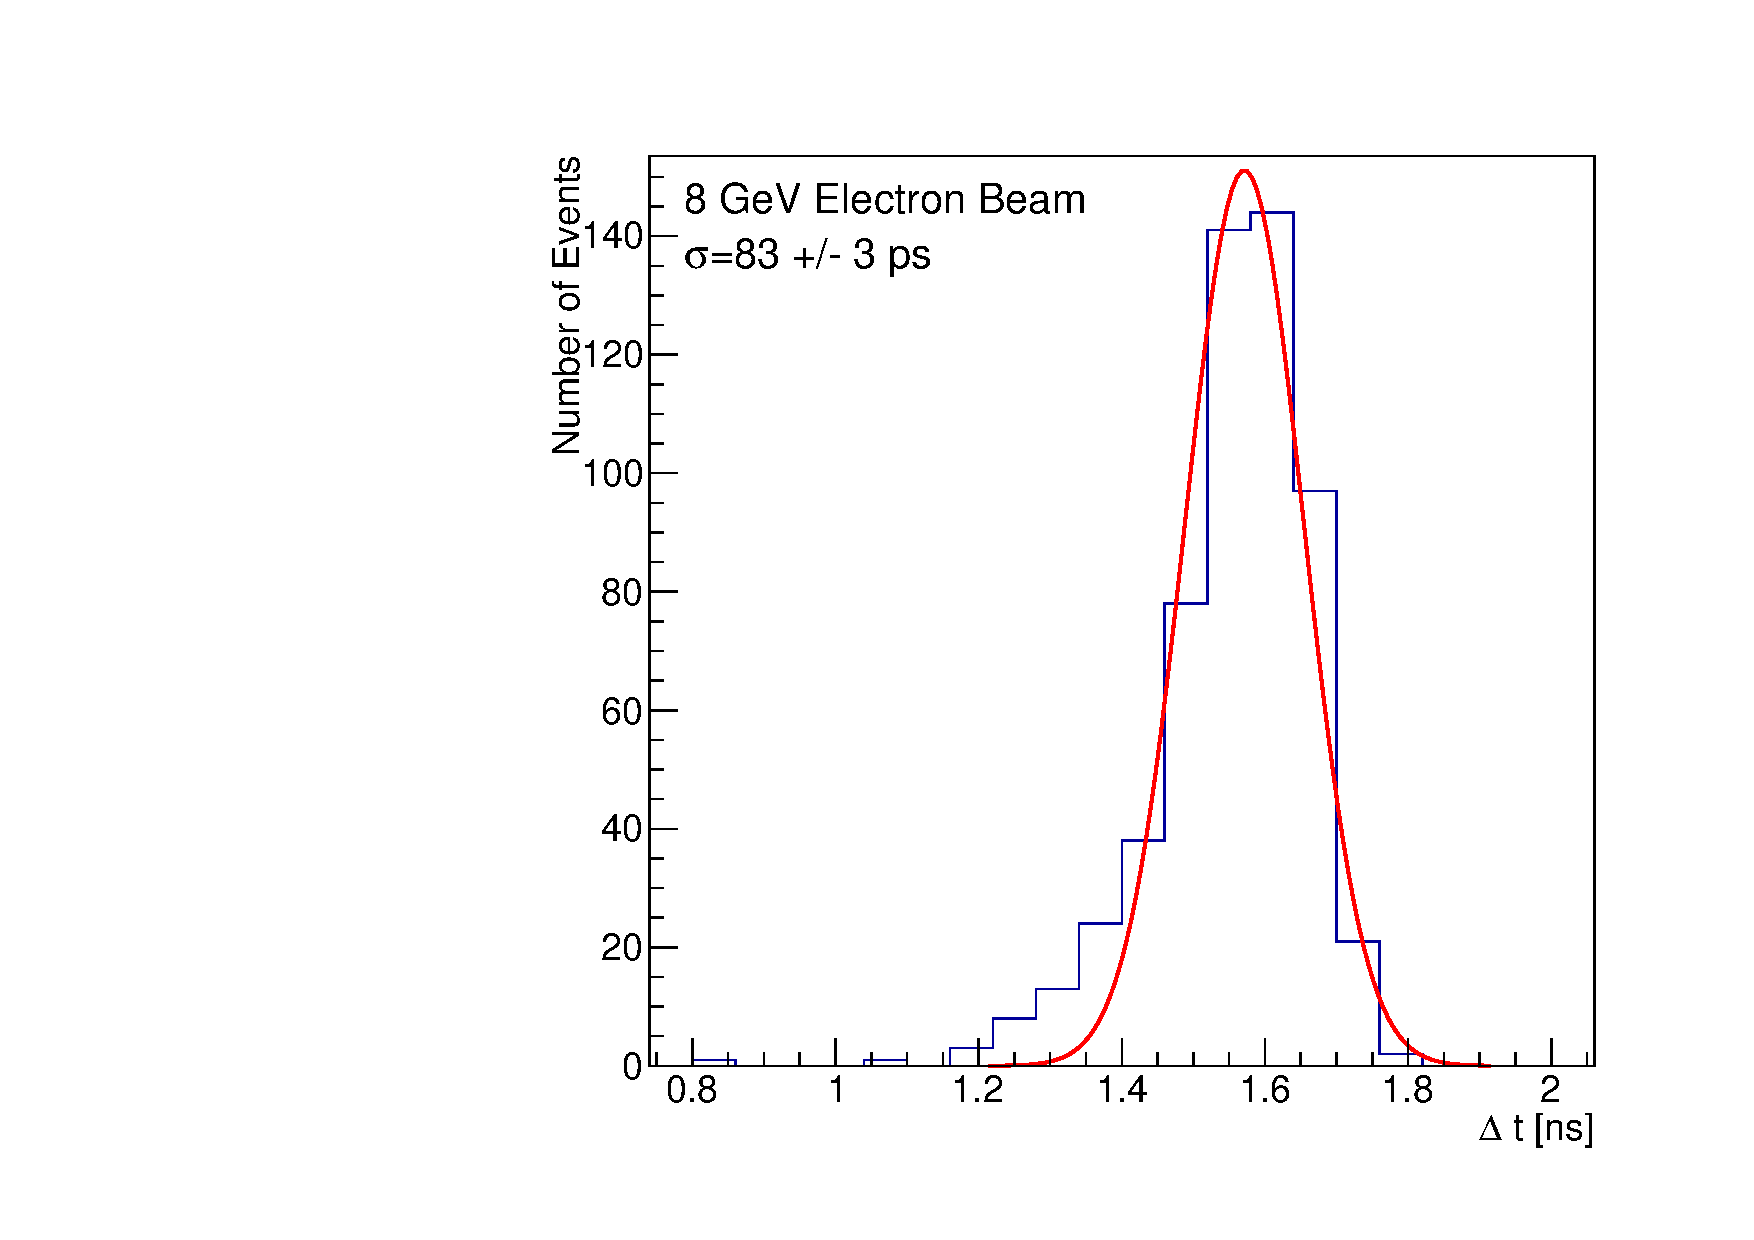
\includegraphics[width=0.45\textwidth]{figs/TOF_ShashlikSideReadout_Electron_8GeV} 
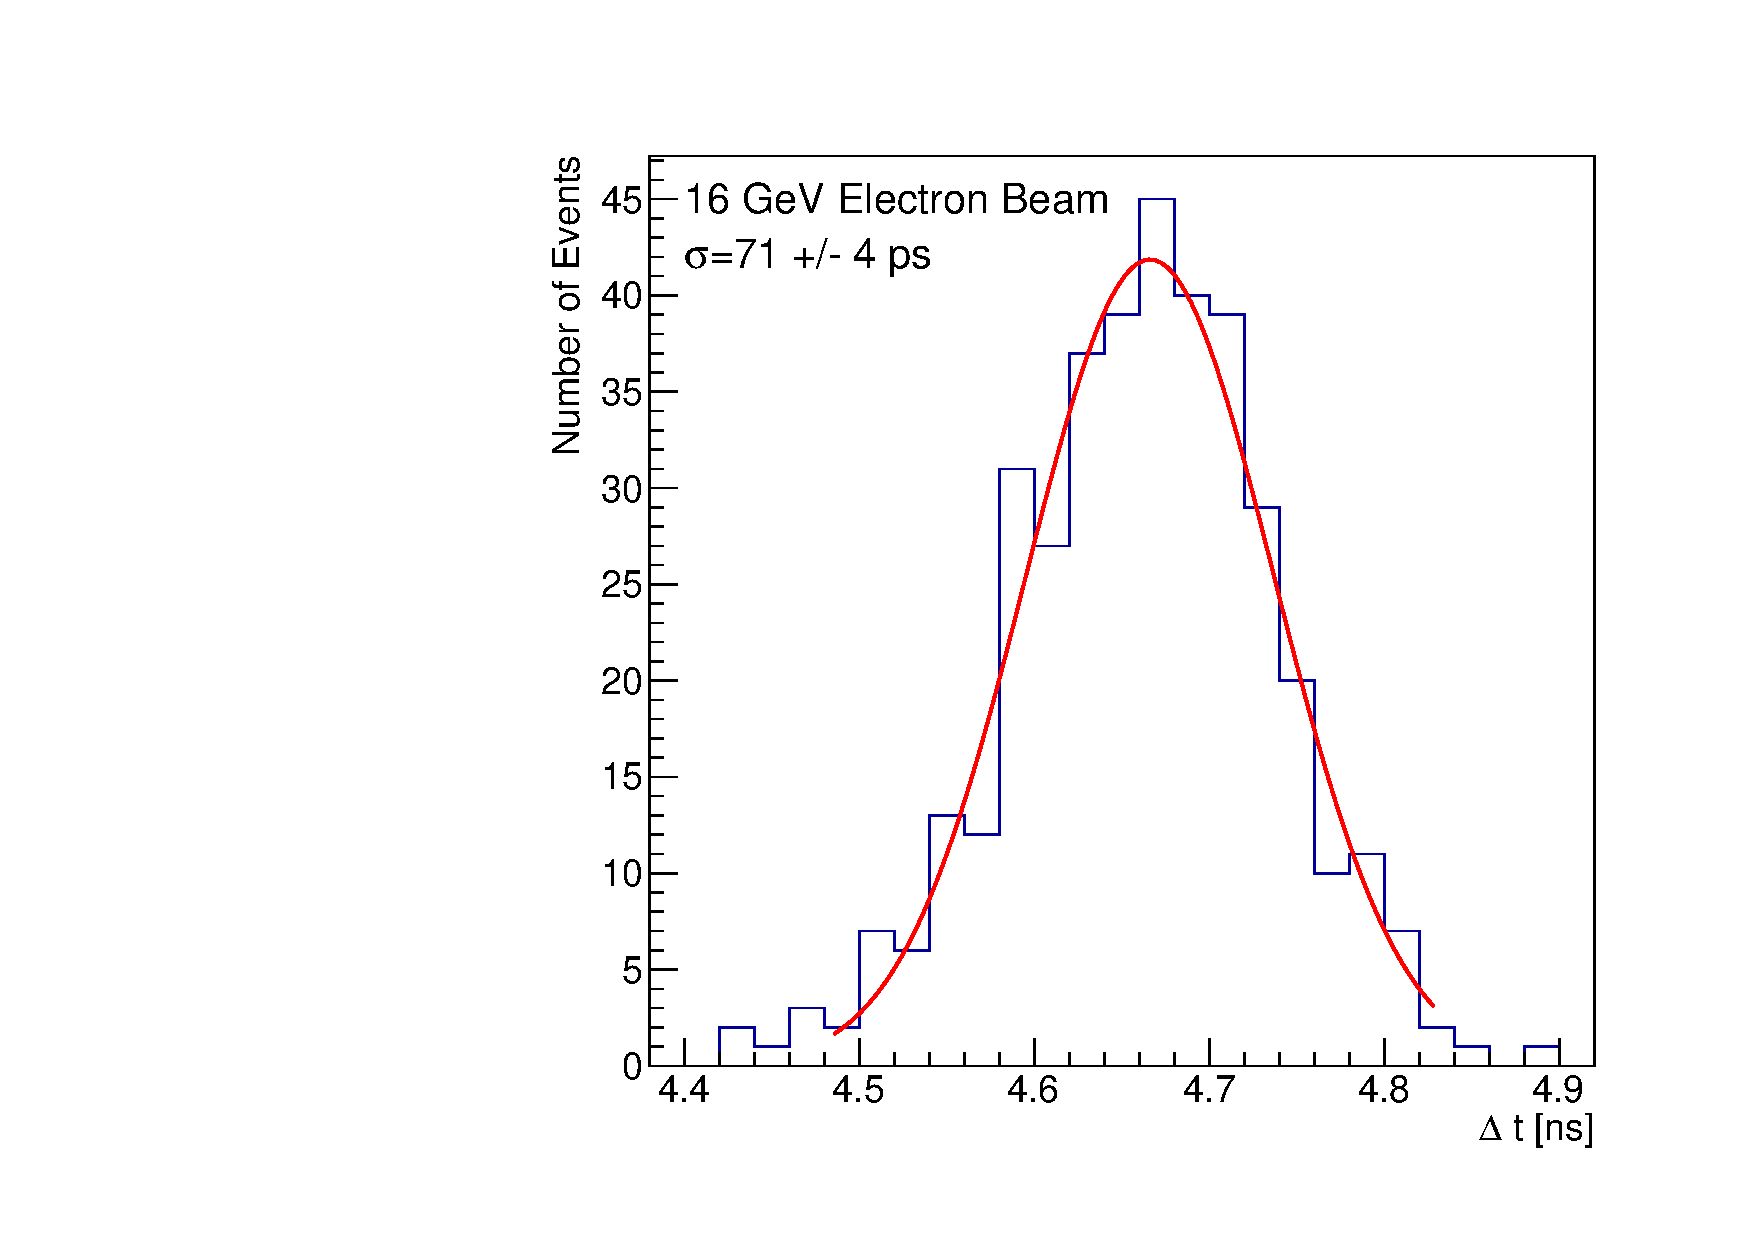
\includegraphics[width=0.45\textwidth]{figs/TOF_ShashlikSideReadout_Electron_16GeV} 
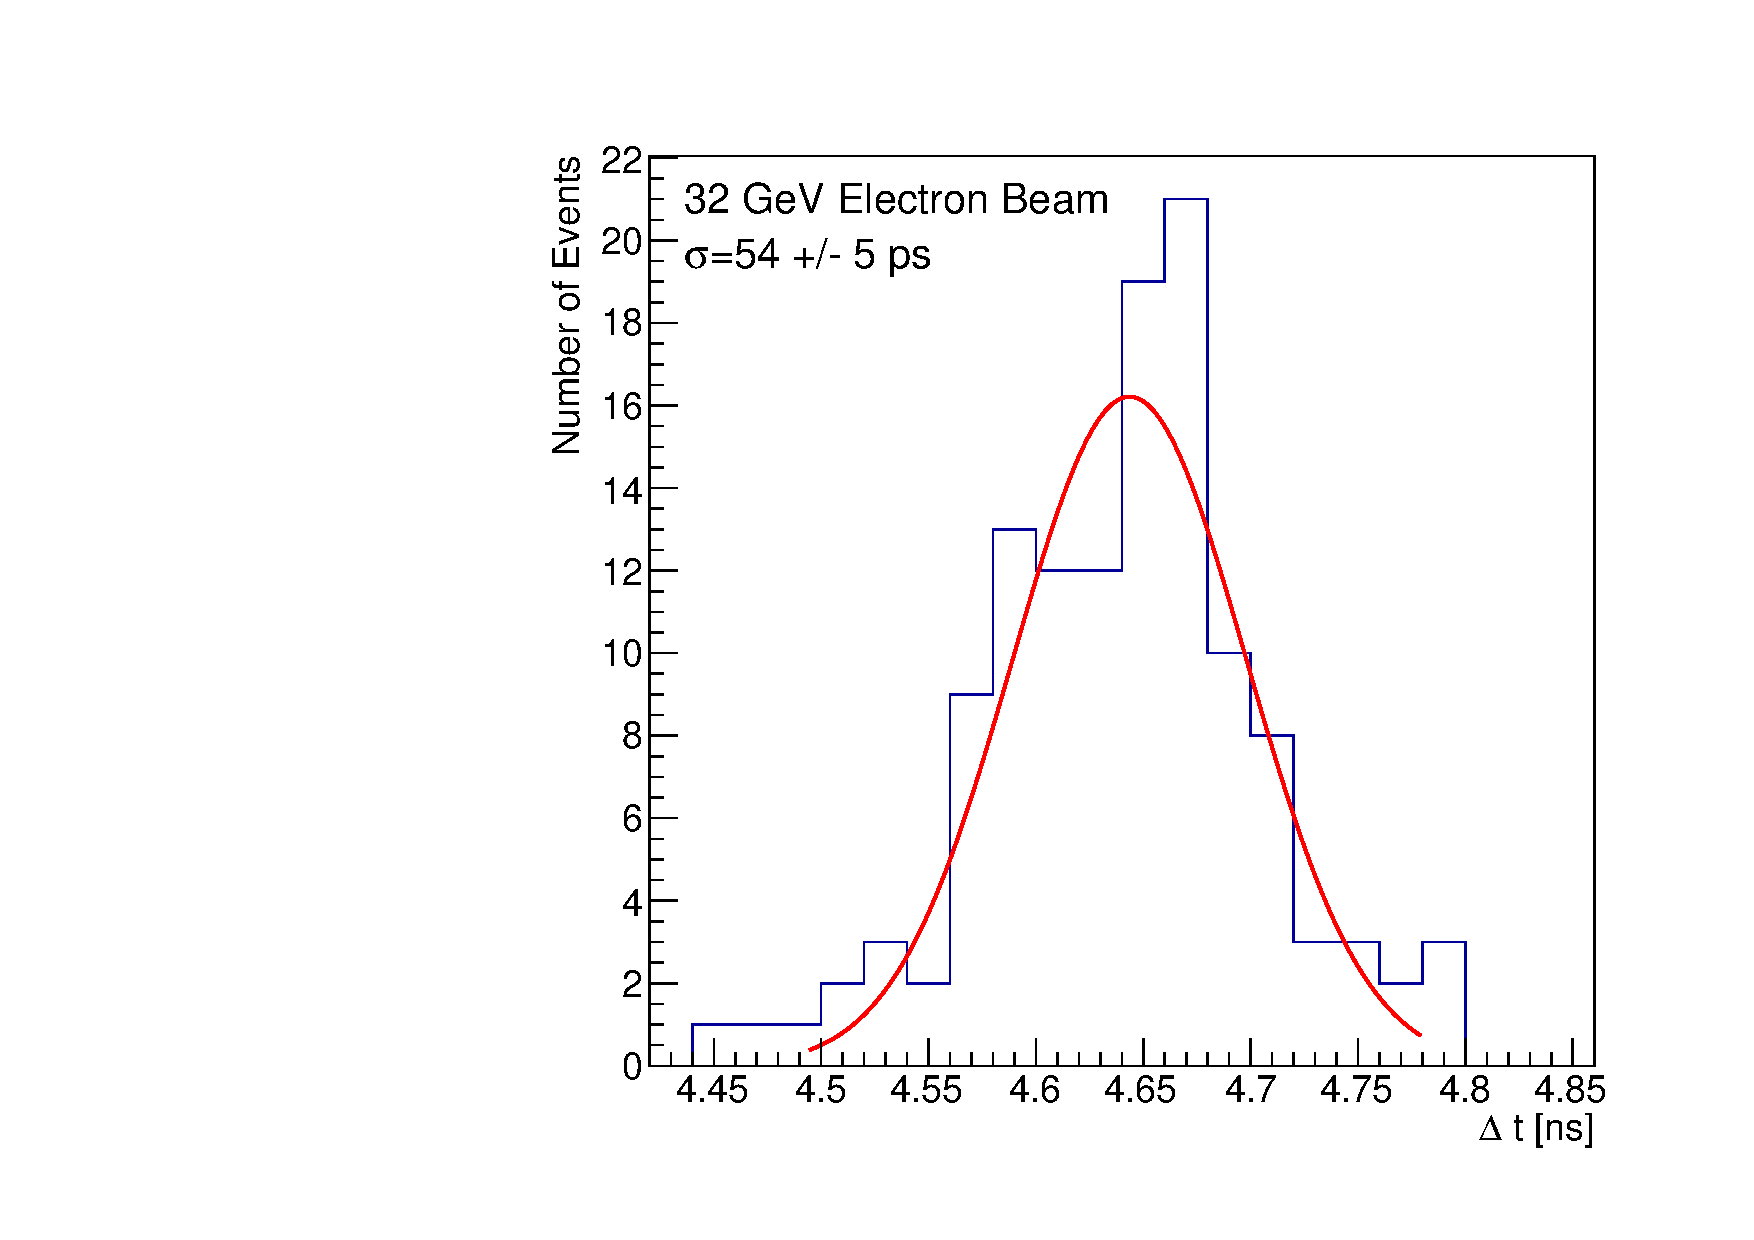
\includegraphics[width=0.45\textwidth]{figs/TOF_ShashlikSideReadout_Electron_32GeV} 
\caption{ Time of flight distributions for the LYSO-tungsten shashlik calorimeter
with signal extracted from the edges of two LYSO layers. } 
\label{fig:ShashlikSideReadoutTOF}
\end{figure}

\begin{figure}[H] \centering
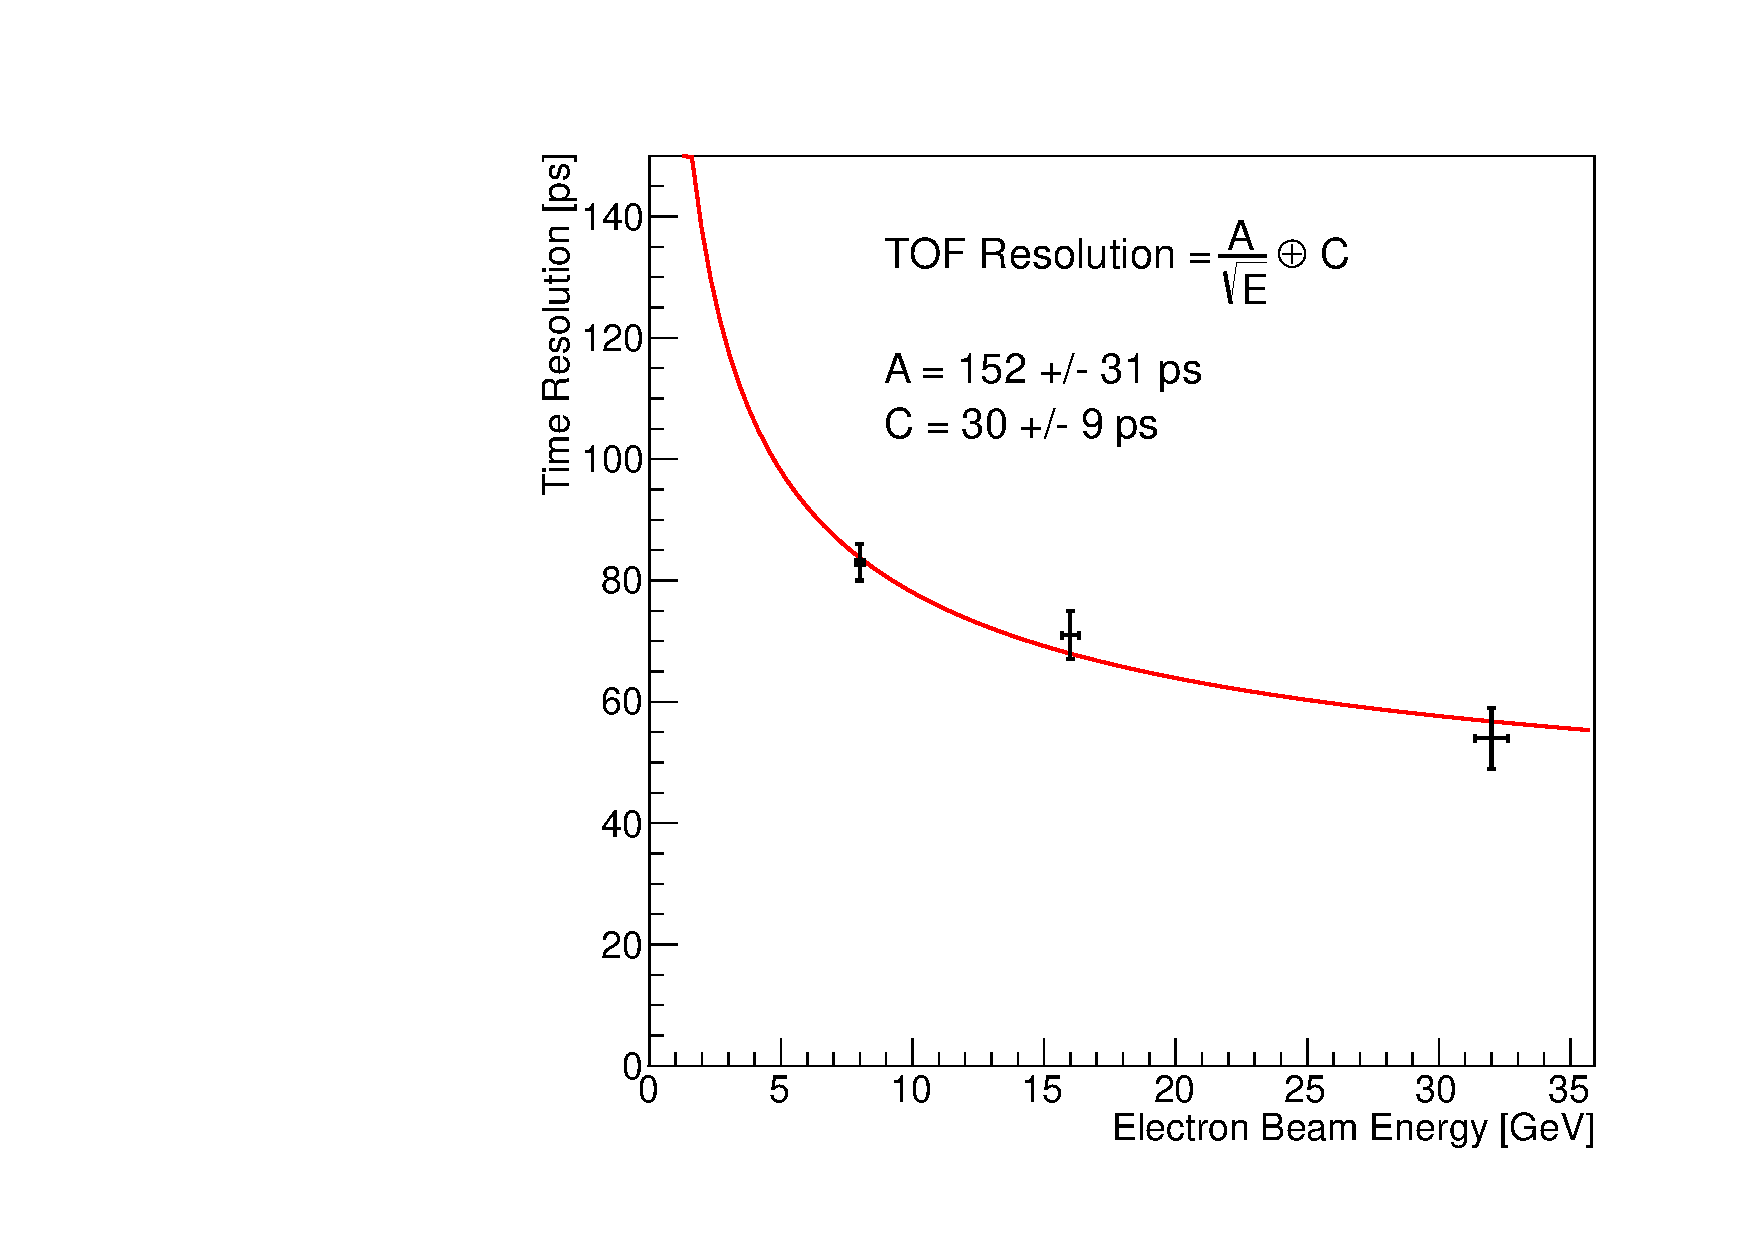
\includegraphics[width=0.45\textwidth]{figs/TimeResolutionVsEnergy_ShashlikSideReadout} 
\caption{ The time resolution measured using the LYSO-tungsten shashlik calorimeter
with light signals extracted by direct optical coupling to the edges of two LYSO layers 
is plotted as a function of the electron beam energy, and fitted to the sum 
of a $1/\sqrt{E}$ term and a constant term. }
\label{fig:ShashlikSideReadoutTOFResolutionVsEnergy}
\end{figure}

In summary, we find that removing the impact of the wavelength shifting mechanism
and minimizing the impact of the optical transit does indeed improve the time
 resolution, but at a cost in photostatistics. Results obtained in this
experiment suggest that the LYSO-tungsten shashlik calorimeter with edge
signal readout design can likely achieve a $30$~ps resolution provided 
some improvement to light collection is achieved.

\section{Summary}

In this article we have described studies characterizing the 
performance of time of flight measurements using
LYSO-based calorimeteric detectors. Using a $(1.7\mathrm{ cm})^{3}$
LYSO crystal that samples the electromagnetic showers created
by electrons of various energies ranging from $4$~GeV to $32$~GeV
at about $4.5$~$X_{0}$, we infer that the contribution to the 
time  resolution due to event-by-event fluctuations 
of the scintillation process is less than $20$~ps. Studies of the
effect of optical transit through the use of wavelength shifting
fibers in a LYSO-tungsten Shashlik calorimeter demonstrated that
the choice of WLS fiber has a major impact on the timing performance.
Besides the details of the absorption and re-emission processes in
the WLS fibers, we find that another important factor on
the timing performance is the light extraction efficiency. Using
the superior performing DSB1 fibers, we obtain a best time
resolution of about $100$~ps, and find that the time
resolution remains photo-statistics limited.
Therefore future improvements on the performance of such a 
detector will need to focus on improvements to the light collection
efficiency. Finally, using a scheme where the scintillation
light from the LYSO-tungsten Shashlik calorimeter is extracted
via the edges of two LYSO layers, thereby removing the impact
of the wavelength shifting mechanism, we achieve a best time  resolution of $55$~ps. This result gives some indication that such a
calorimeter design would likely be able to achieve a $30$~ps 
time  resolution provided some improvement to the 
light collection efficiency can be achieved.

Combined with the results of reference~\cite{MCPFastCaloNIMA}, we 
have completed the characterization of the main factors
contributing to the time  resolution in a LYSO-based
calorimeter. The effects of event-by-event fluctuations in
the electromagnetic shower as well as the scintillation process 
are controlled to within $20$~ps. The effects of the optical transit
can be controlled to within $20$ or $30$~ps, depending on the
exact scheme for extracting the light signal. Through the comparison of results
using these different light extraction schemes, we find that at a 
given light yield the effect of optical transit fluctuations
is of considerable importance, but that these effects
have a tendency to decrease in importance as the light yield
increases. This effect can be seen in 
Figure~\ref{fig:ShashlikFiberAndCubeTOF} where we show
the dependence of the time resolution
for the shashlik cell with light extraction through the
DSB1 fibers and for the sampling calorimeter with the
$(1.7$~cm$)^{3}$ LYSO cube as active element as a function
of the average pulse height. At the same average pulse height,
a difference of a factor of two is observed in the
measured time  resolution, primarily due to
optical transit effects. However, as the pulse height
increases, the time  resolution also improves.
Extrapolating to the regime of very large light yield,
we have not observed any evidence of an
ultimate limitation in resolution resulting from
optical transit fluctuations.

\begin{figure}[H] \centering
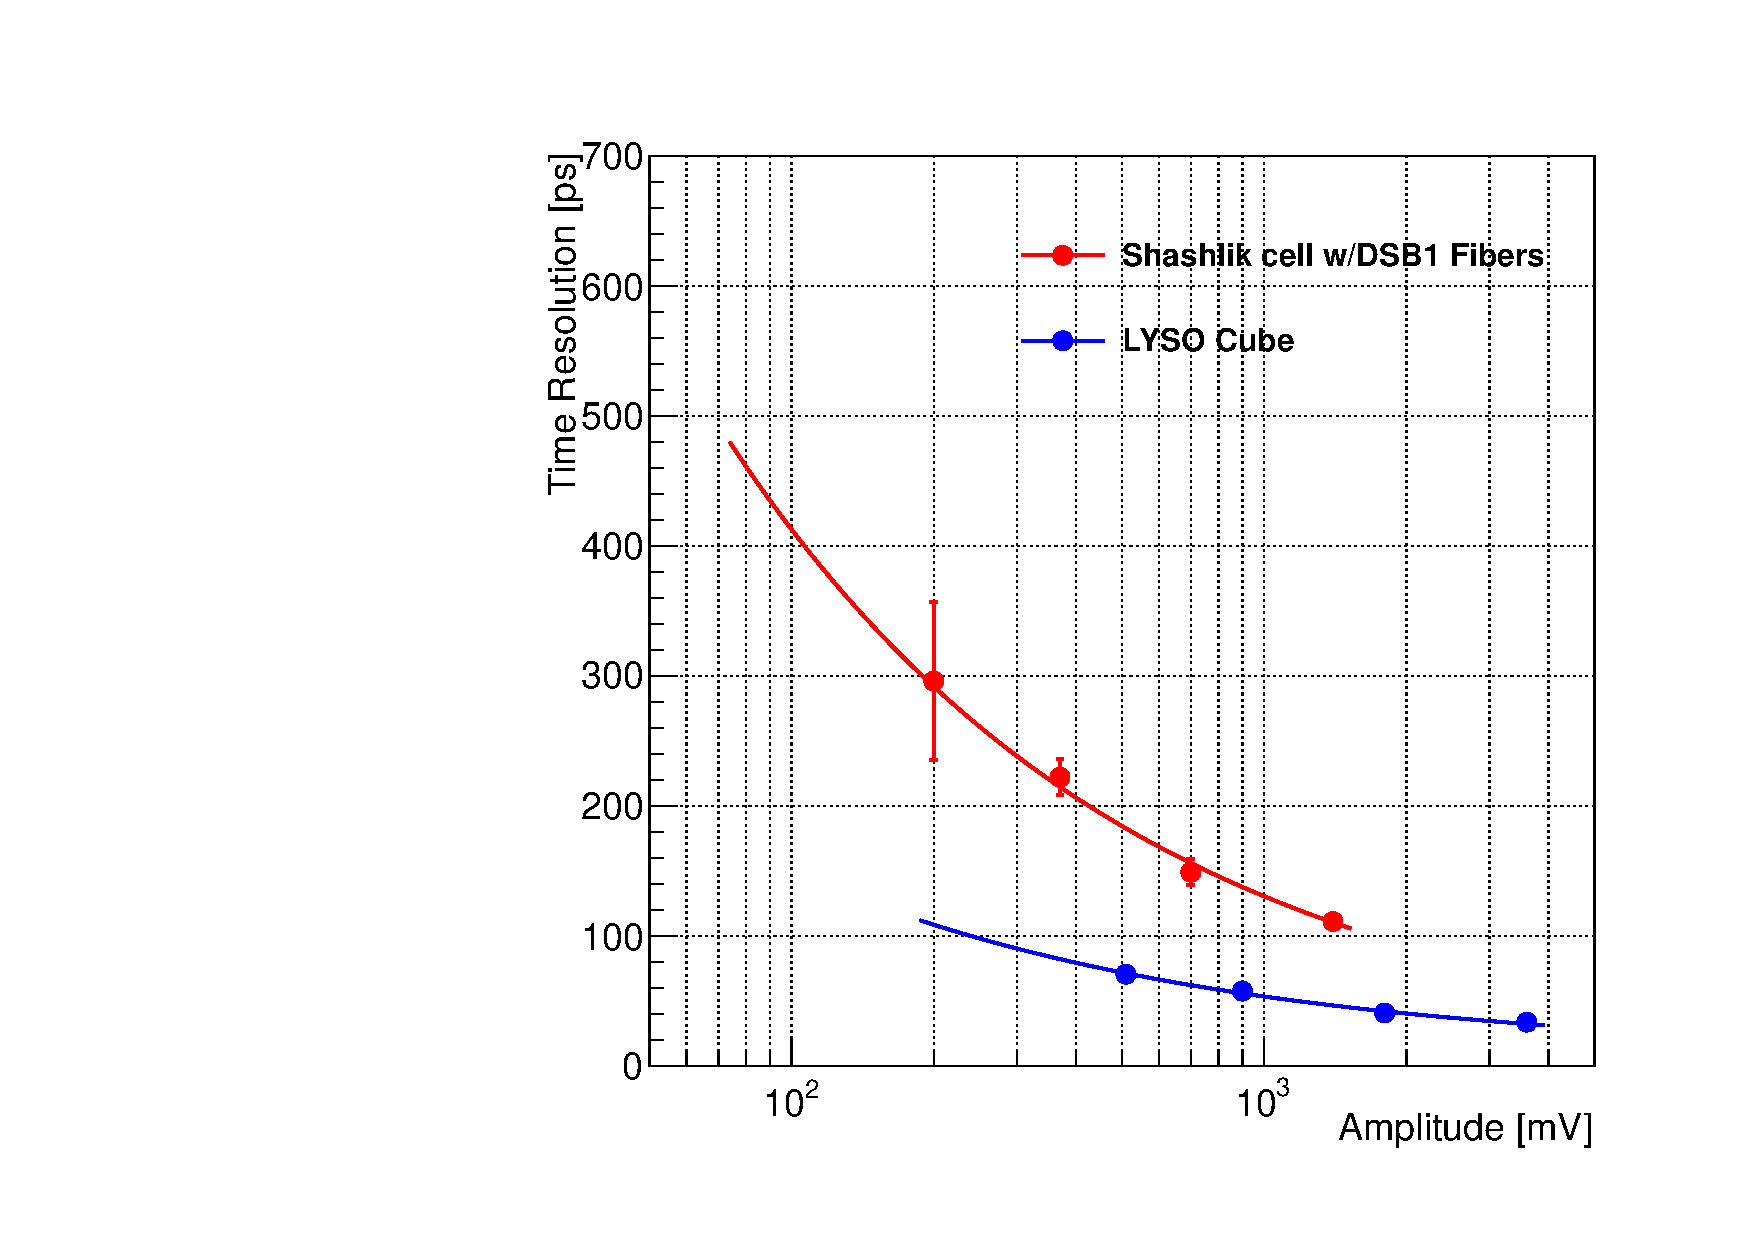
\includegraphics[width=0.55\textwidth]{figs/TimeResolutionVsEnergy_ShashlikDSB1FiberAndCube} 
\caption{Comparison of time resolutions obtained with the 1.7 cm$^3$ LYSO cube (blue), and the LYSO-tungsten shashlik calorimeter with light extracted using DSB1 fibers (red). Note that x-axis in this figure displays the amplitude of the signal as measured by the DRS4 board.} 
\label{fig:ShashlikFiberAndCubeTOF}
\end{figure}

In summary, at the light yield achieved all factors can be controlled
to within $30$~ps, and the goal of obtaining $30$~ps
resolution time measurements using a LYSO-based calorimeter
is achievable. The next step will be to further 
investigate any ultimate limitation in time 
resolution in the limit of very large light yield,
and to make improvements to the light collection efficiency 
for such types of detectors.

\section{Acknowledgements}
We would like to thank Erik Ramberg and Sergey Los for their support of our work, and Aria Soha and the FTBF test beam facility for the
good beam delivery and control. We thank Randy Ruchti for providing us
with the DSB1 fibers used in the measurements, and Eileen Hahn for the
high quality work in polishing the fibers. Thanks to Ewa Skup and Geoff
Savage for help with operation of Cherenkov counters, and to Todd Nobel
for organizing and providing supporting equipment at FTBF.


\bibliography{FastTimingPaperAug2014}{}
\bibliographystyle{ieeetr}
\end{document}    
        






























